

\documentclass[12pt,letterpaper]{article}

\usepackage{setspace}
%\doublespacing
%\linespread{1.25}
\linespread{2}
\usepackage{geometry}
 
\geometry{letterpaper, margin=1in}
%\usepackage{times}
\usepackage{pslatex}
\usepackage{apacite}
\usepackage{url}
\usepackage{graphicx}
\usepackage{caption}
\usepackage{subcaption}
\usepackage{listings}
\usepackage{color}
\usepackage{textcomp}
\usepackage{amsmath}
\usepackage{amssymb}
\usepackage{wrapfig}
\usepackage{lipsum}
\usepackage{setspace}

\usepackage{fancyhdr}
\pagestyle{fancy}
\renewcommand{\headrulewidth}{0pt}
\fancyhf{}
\fancyhead[R]{\thepage}
\lhead{\textsc{pragmatic theory of generic language}}

\graphicspath{{../figures/}}
  
\def\signed #1{{\leavevmode\unskip\nobreak\hfil\penalty50\hskip2em
  \hbox{}\nobreak\hfil(#1)%
  \parfillskip=0pt \finalhyphendemerits=0 \endgraf}}

\newsavebox\mybox
\newenvironment{aquote}[1]
  {\savebox\mybox{#1}\begin{quote}}
  {\signed{\usebox\mybox}\end{quote}}


 \newcommand{\denote}[1]{\mbox{ $[\![ #1 ]\!]$}}

\definecolor{Red}{RGB}{255,0,0}
\newcommand{\red}[1]{\textcolor{Red}{#1}}  
\definecolor{Green}{RGB}{10,200,100}
\definecolor{Blue}{RGB}{10,100,200}
\newcommand{\ndg}[1]{\textcolor{Green}{[ndg: #1]}}  
\newcommand{\mht}[1]{\textcolor{Blue}{[mht: #1]}}  

\usepackage{titlesec}

\setcounter{secnumdepth}{4}

\titleformat{\paragraph}
{\normalfont\normalsize\bfseries}{\theparagraph}{1em}{}
\titlespacing*{\paragraph}
{0pt}{3.25ex plus 1ex minus .2ex}{1.5ex plus .2ex}

\title{A pragmatic theory of generic language}
%\title{Generics are vague: A formal theory of generalizations in language}
%\title{Generics are vague: a probabilistic model of generic language}
%\title{Generic language is vague yet rationally understood}
%\title{Generic language is vague yet pragmatically understood}
%\title{Generic language is vague yet pragmatically used}

\author{{\large \bf Michael Henry Tessler} (mtessler@stanford.edu)\\ {\large \bf Noah D. Goodman} (ngoodman@stanford.edu) \\
  Department of Psychology, Stanford University}
  
 \date{}
\begin{document}

\maketitle

%A Pragmatic Theory of Generic Language 

Running head: \textsc{pragmatic theory of generic language}

\vspace{80 mm}
{\setstretch{1.0}
\textsc{\\corresponding author \\
Michael Henry Tessler \\
Stanford University, Department of Psychology \\
450 Serra Mall, Bldg. 420, Rm. 316 \\
Stanford, CA 94305 \\
mtessler@stanford.edu \\
757 - 561- 7071}

}
\newpage
%\contributor{Submitted to Proceedings of the National Academy of Sciences
%of the United States of America}

%%%Newly updated.
%%% If significance statement need, then can use the below command otherwise just delete it.

%
%\significancetext{
%Understanding the world requires making generalizations about categories; we use generic language to convey such generalizations: `dogs bark', `rats carry disease', and `liberals drink lattes'.
%These simple sentences are common in ordinary conversation, child-directed speech, and political discourse.
%They are how we teach, how we motivate, and how we persuade (or mislead) others.
%Yet the precise meaning of generics is a puzzle that has resisted formalization.
%We introduce a mathematical model of generic language by combining principles of language understanding with a basic meaning in terms of property statistics.
%This theory provides the connective tissue between generic language and conceptual knowledge and gives insight into how everyday language use is tied to beliefs. 


%of the parties involved.
%
%Understanding the world requires making generalizations about categories.
%Generic language (e.g. \emph{Dogs bark.}) provides an efficient and ubiquitous way to transmit this kind of information.
%Yet, these common, simple sentences that even 2-year-olds can comprehend have philosophically puzzling qualities which have impeded precise formalization. 
%We explain the apparent paradoxes using a meaning of generic language that is simple but underspecified. 
%With uncertainty in the language, general principles of communication and 
%interlocutors' shared beliefs about the categories and properties in question 
%are responsible for establishing a precise meaning in context.
%This theory provides the connective tissue between generic language and conceptual knowledge and demonstrates 
% how beliefs play a foundational role in understanding language. 
 %
 % We find this model to explain almost all of the variance in human judgments of the acceptability of familiar generic sentences and 
% to human interpretations of unfamiliar generic sentences.
%to others forms the fabric of conceptual developmental and cultural transmission.
%Utterances that convey generalizations----generic utterances----are ubiquitous in everyday conversational and child-directed speech, 
%yet there is to date no formal account of their precise meanings.
%Humans build internal representations of the world by making generalizations about categories, and use language to convey these generalizations to 
%M.H.T. and N.D.G developed theory and designed research; M.H.T. performed research and analyzed data. M.H.T. and N.D.G. wrote the paper.
%}

%\maketitle

\begin{abstract}
{Generalizations about categories are central to human understanding, and generic language (e.g.~\emph{Dogs bark.}) provides a simple and ubiquitous way to communicate these generalizations. 
Yet the meaning of generic language is philosophically puzzling and has resisted precise formalization.
We explore the idea that the core meaning of a generic sentence is simple but underspecified, 
and that general principles of pragmatic reasoning are responsible for establishing the precise meaning in context.
Building on recent probabilistic models of language understanding, we provide a formal model for the evaluation and comprehension of generic sentences. 
This model explains the puzzling flexibility in usage of generics in terms of diverse prior beliefs about properties.
We elicit these priors experimentally and show that the resulting model predictions explain almost all of the variance in human judgments for both common and novel generics.
This theory provides the mathematical bridge between the words we use and the concepts they describe.
}
\end{abstract}

\newpage
%\keywords{generic language | semantics | pragmatics | categories}

Most would agree that \emph{Swans are white}, but certainly not every swan is.
This type of utterance conveys a generalization about a category (i.e. \textsc{swans}) and is known as a generic utterance \cite{Carlson1977,Leslie2008}.
Category knowledge is central to human reasoning \cite{Markman1989}, but is hard to come by because categories themselves are unobservable.
%yet attaining such knowledge is tantamount to solving problems of induction \cite{Hume1888}. 
%Generic utterances shortcut such inductive problems by conveying the generalization from speaker to hearer.
It is believed that every language can express generic meaning \cite{Behrens2005,Carlson1995}, and that generics are essential to the growth of conceptual knowledge \cite{Gelman2004} and how kinds are represented in the mind \cite{Leslie2008}.
Generic language is ubiquitous in everyday conversation as well as in child-directed speech \cite{Gelman2008}, and children as young as two or three understand that generics refer to categories and support generalization \cite{Cimpian2008}.
% and though English and many other languages do not possess an unambiguous form devoted to generic meaning \cite{Behrens2000, AlMalki2014}. 
Additionally, generics are the primary way by which speakers discuss social categories, making them key to propagating stereotypes \cite{GelmanEtAl2004,Rhodes2012,Leslie2015} and impacting motivation \cite{Cimpian2010motivation}.
Despite their psychological centrality and apparent simplicity, a formal account of generic meaning remains elusive.

The major issue in formalizing generic language is determining what makes a generic sentence true or false.
At first glance, generics seem like universally-quantified statements as in \emph{All swans are white}, but unlike universals, generics are resilient to counter-examples (e.g. \emph{Swans are white} even though there are black swans). 
Interpreting the generic as meaning ``most'' (i.e. \emph{Most swans are white}) captures many cases, but cannot explain why \emph{Robins lay eggs} and \emph{Mosquitos carry malaria} are so intuitively compelling: Only adult female robins lay eggs and a very tiny fraction of mosquitos actually carry malaria.
Indeed, it appears that any explanation in terms of how common the property is within the kind violates intuitions --- for the robins, laying eggs is practically synonymous with being female (i.e., the properties are present in the same proportion), yet \emph{Robins are female} is not a reasonable utterance while \emph{Robins lay eggs} is fine.

% as , even though the two properties are present in the same proportion (about 50\%) in the category of robins.
%\ndg{No precise meaning formalized in the mathematical language of logic seems to be sufficient to capture the meaning of natural language generics.}

%Generics are additionally puzzling in how they are interpreted. 
%The mystery deepens with how generic language is interpreted.
How generic language is interpreted is also a mystery.
%The strong interpretation of novel generics deepens the mystery.
\emph{Mosquitos carry malaria} suggests the generic must in some way be analogous to ``some'' (i.e. \emph{Some swans are white.}). 
Yet generics are often interpreted as implying the property is widespread within the kind:
%Yet generics often imply the property is widespread: 
%Listeners often interpret a novel generic as applying to \emph{nearly all} of a category 
Consider the difference between \emph{Some swans have hollow bones} and \emph{Swans have hollow bones} \cite{Gelman2002}.
When asked how common a property would need to be for the generic utterance to be true, both children and adults require the property to be less widespread than they infer when told the generic \cite{Cimpian2010,Brandone2014}, suggesting that communicating with generics can exaggerate evidence.
%Both children and adults believe the generic implies the property-in-question is even more widespread than when asked how common the property would need to be for the generic to apply

How can generics have such flexible truth conditions while simultaneously carrying strong implications?
In this paper we resolve these philosophical and empirical puzzles using a mathematical model that understands generic language by pragmatic inference about the degree of prevalence required to assert the generic.  
This model predicts the patterns in both human endorsement of familiar generic sentences and interpretation of novel generic sentences. 

\subsection*{The semantics and pragmatics of generic language}


Generics express a relation between a kind K (e.g. \textsc{robins}) and a property F (e.g. \textsc{lays eggs}). 
These often take the form of a bare plural (e.g. \emph{Ks have Fs}), which lack explicit quantifiers or determiners \cite{Carlson1977}.
Semantic theories of generics aim to unify the diverse meanings associated with this simple, syntactic construction. 
\citeA{Carlson1977} hints at what is necessary:
%
\begin{quote}
What is suggested, then, is that the apparent variation in ... truth-conditions .. can be attributed to our \emph{strategies of investigation} and not to any inherent semantic marker in the sentence (in particular, a quantifier). [emphasis ours]
\end{quote}
%
For \citeauthor{Carlson1977}, there are different \emph{strategies} to verify if a kind has a particular type of property 
(e.g. to verify if a kind \emph{lays eggs} one can employ the strategy to consult only the female members of the kind). 
Later accounts developed this argument to appeal to structured, conceptual representations (e.g. \emph{Bishops move diagonally} not because most bishops do but because the laws of chess mandate that they do). 
These stand in contrast with semantic theories of generics that appeal to the statistics of the world (e.g. \emph{Barns are red} because most barns are; \citeNP{Carlson1995essay}).
We review both classes of accounts below.
%(Incidentally, he argued that this was incompatible with the generic being analogous to a quantifier, a point we will dispute.)
%Since that time, there have been many other accounts of generics. 
%We follow \citeA{Carlson1995essay}, and organize the extant theoretical literature by theories that appeal to either the statistics of the world (e.g. \emph{Barns are red} because most barns are) or 
\subsubsection*{Conceptual accounts of generics}

The ``conceptual'' perspective emphasizes the structure of generic knowledge \cite{Prasada2000}, and views generic utterances as the way of expressing special mental relationships between kinds and properties \cite{Leslie2008, Prasada2012}. 
\citeA{Leslie2007} introduces the notion that generics are tied to a ``default mode of generalization''. 
This ``default mode'' comes equipped with the ability to single-out \emph{striking properties} (e.g. properties which are dangerous or appalling) as particularly useful aspects of the world to know about. 
This is the reason why \emph{Mosquitos carry malaria} seems true: It is a useful bit of information to convey.
\footnote{\citeauthor{Leslie2007} goes on to say that this argument depends also on the fact that non-malaria carrying mosquitos must have the potential to carry malaria, and this is why \emph{Insects carry malaria} or \emph{Animals carry malaria} do not seem as good of utterances.}
For properties that are not striking (e.g. in \emph{Barns are red}), then statistical information must be consulted: If the majority of K have F, then the generic is judged to be true. Finally, \citeauthor{Leslie2007} invokes the distinction between ``negative'' and ``positive'' counter-instances. A negative counter-instance is one that is characterized by ``not having F'' (e.g. a bird that doesn't lay eggs) whereas a positive counter-instance is one that is characteristic by ``having not-F'' (e.g. a hypothetical bird that bears live young). Here, it is argued that when positive counter-instances exist, we are much less likely to accept the generic (e.g. \emph{Birds are female} seems weird because ``being male'' is a positive counter-instance of ``being female''). 
When there are only negative counters-instances, the generic is acceptable (e.g. \emph{Birds lay eggs.} since there no such birds that bear live young).

This account has support in the empirical literature.
\citeA{Prasada2006} distinguish between \emph{statistical} and \emph{principled relations} within concepts. 
These distinct relation types manifest themselves empirically as different inferences one could draw concerning the kind and property. 
For example, these include the expectation that the relation will hold for future instances (operationalized using the phrase \emph{In general, Ks have F}), the explanation that the relation holds because of the kind of thing that K is (\emph{Ks have F by virtue of being a K}), and that the principled relation is normative (\emph{Ks should have Fs}).
These different kinds of relations relate to \citeA{Leslie2007}'s distinctions among generics.
For instnance, \citeA{Prasada2013} found generics like \emph{Birds lay eggs} (in which only a minority of K have F) exhibit characteristics of principled connections. 
Striking generics (e.g. \emph{Mosquitos carry malaria}) do not have the characteristics of principled connections, but do show characteristics of a third kind of connection: a \emph{causal connection} (operationalized using the phrase \emph{There is something about Ks that cause them to F}). 
Different kinds of kind--property relations exhibit qualitatively different kinds of connections. 
This is taken to support \citeA{Leslie2007}'s typology of different types of default generalizations.

%The puzzles of generic language then reduce to puzzles about mental representation of kind-property relations.


\subsubsection*{Statistical accounts of generics}

Not all accounts of generic language reduce to puzzles about mental representation of kind--property relations.
Accounts stemming from formal semantics tend to look towards precise, quantifiable conditions to determine if a sentence is true or false.
The most promising account of generics in this tradition was put forth by \citeA{Cohen1999}.
To understand this theory, let's introduce some notation:

For a given kind $K$ (e.g.~\textsc{robins}) and property $F$ (e.g.~\textsc{lays eggs}), we refer to the probability that an object of kind $K$ has property $F$, that is $P(F\mid K)$, as the \emph{prevalence} of $F$ within $K$.
Logical quantifiers can be described as conditions on prevalence (i.e.~\emph{some} is $P(F\mid K)>0$, \emph{all} is $P(F\mid K)=1$). 
Assuming the generic relates to the property prevalence, then the simplest meaning would similarly be a threshold on prevalence: $P(F\mid K)>\tau$. \citeA{Cohen1999} takes $\tau = 0.5$; that is, \emph{Robins lay eggs} is roughly taken to mean \emph{Most robins lay eggs}. 

Of course most robins do not lay eggs; none of the male robins do. Cohen resolves this issue by introducing certain constraints into the computation of prevalence: $P(F\mid K)$. In particular, prevalence is computed with respect to a \emph{partition set}. In this theory, \emph{lays eggs} induces a set of alternatives that all have to do with procreation (e.g. \emph{gives birth to live young}, \emph{undergo mitosis}, ...). Then, the individuals that enter into the prevalence computation are only those individuals that would satisfy one or another alternative. 
That is, the only individuals under consideration are the female members of kinds because only the female members could plausibly satisfy one of the alternatives.
Thus, \emph{Birds lay eggs} is roughly taken to mean \emph{Most female birds lay eggs}. 

Other constraints enter into the computation of prevalence as well (e.g. further partitions with respect to time). 
The theory, though mathematically rigorous and rationally appealing, relies upon a number of a working parts that need to be determined in some (unspecified) way by pragmatics. 
In addition, it is unclear how to get from this semantic theory to the unspecified pragmatic theory on which it relies.
More generally, how this semantic theory relates to the conceptual accounts of generics also remains obscure (however, see \citeNP{Cohen2004} for a discussion of how his semantic constraints relate to different kinds of generics and different kinds of conceptual representational frameworks used in cognitive science).


%If this is the case, then a relatively simple semantic theory, phrased in terms of statistical regularities in the world, could be enough to formalize generic language.
%Abstract, mental representations may still operate; yet we suggest generic language operates through the common currency of probability. 

\subsubsection*{The current approach}

We aim to unify the ``statistical'' and ``conceptual'' ways of understanding generic language. 
We begin by noting that generic language is not unique in its flexibility.
Language understanding in general depends on assumptions interlocutors make about each other and what content is under discussion. 
Pragmatic analyses reveal that utterances carry a mosaic of interpretations with a complex sensitivity to context \cite{Clark1996,Grice1975,Levinson2000}. 
Can the puzzles of generic language be understood as effects of pragmatic reasoning?
If so, it may be unnecessary to encode abstract mental representations% and complex computational constraints 
into the semantics of generics.
Abstract representations, however, may be the backdrop against which generic language gets interpreted. 

We propose a relatively simple semantic theory, phrased in terms of statistical regularities.
Following \citeA{Cohen1999}, we measure these regularities with probability and adopt the simplest meaning for generic statements: a threshold on prevalence: $P(F\mid K)>\tau$.\footnote{Because we aim to explain the psycholinguistics of generics, we are generally interested in the subjective probability, not the actual frequency in the world.}
Of course, no fixed value of the threshold, $\tau$, allows for the extreme flexibility generics exhibit (e.g. \emph{Robins lay eggs} vs. \emph{Robins are female}; \emph{Mosquitos carry malaria}).% simultaneously with the interpretations of some novel generics being strong. 

We suggest that this threshold is not a fixed property of the language, but is established in context through communicative principles.
This inference depends on background knowledge about properties and categories, but is otherwise a general mechanism of language not specific to interpreting generic statements.
We formalize this inference in the Rational Speech-Acts (RSA) theory---a probabilistic model of language understanding---as recursive Bayesian inference between speaker and listener \cite{Frank2012,Goodman2013}.
We will describe the basic RSA framework before articulating the full pragmatic theory of generic meaning.

\subsubsection*{The Rational Speech-Acts framework}

The goal of this section is introduce the reader to the Rational Speech-Acts framework and point to various applications and areas of ongoing research when relevant.

The Rational Speech-Acts theory views language understanding as a special case of social cognition instantiated in a Bayesian model \cite{Goodman2013}. 
In this view, an utterance is \emph{interpreted} by a listener consulting her intuitive theory of speech \emph{production}, i.e. her theory of a speaker. This intuitive theory of a speaker has the assumption that speakers choose speech-acts approximately optimally on the basis of certain goals (specifically, the goal of conveying information to the listener). 
A listener then ``inverts'' her model of a speaker and arrives at a pragmatic interpretation of an utterance after taking into account her relevant world knowledge. 
This model is posed at the computational or rational level \cite{Marr1980, Anderson1991}. 
It is not intended as an explicit model of the \emph{process} of language comprehension; rather, it is a computational model of pragmatic competence under the cooperative principle \cite{Grice1975}. 

In simplest form, a pragmatic listener ($L$) is interested in learning about the world $x$ upon hearing an utterance $u$. 
$$
P_{L}(x  \mid u) \propto P_{S}(u \mid x) \cdot P(x) \label{eq:RSA_L}
$$
She does this by integrating her prior beliefs about the world $P(x)$ with the likelihood that a speaker ($S$) would have produced the utterance $u$ given a world $x$: $P_{S}(u \mid x)$.
Prior beliefs about the world $P(x)$ capture relevant world-knowledge, which is central to deriving context-specific interpretations \cite{Degen2015cogsci}.
The production model $P_{S}$ is defined recursively with the listener model: The speaker produces an utterance according to a utility function, which is a soft-max function of the probability that the listener would infer the world $x$ given the utterance $u$: $P_{L}(x  \mid u)$, jointly with the prior probability of the utterance $P(u)$.
$$
P_{S}(u \mid x) \propto P_{L}(x  \mid u) ^\lambda \cdot P(u) \label{eq:RSA_S}
$$
$\lambda$ it the ``speaker optimality'' parameter: It governs the degree to which the speaker values informativity when producing an utterance. The speaker is not perfectly Bayesian because he is assumed to be a rational actor, and takes actions soft-max optimally in accord with his posterior belief distribution \cite{Baker2009}.


The prior probability of an utterance $P(u)$ can include information about an utterance's cost or complexity as well as the alternative utterances available to a speaker. 
Manipulating an utterance's cost has been used to derive Manner implicatures \cite{Bergen2016}, though in many applications utterance cost is kept uniform across alternative utterances. 
The specification of alternatives is an area of ongoing research \cite{Franke2014cogsci, Peloquin2016} and is currently determined by the modeler for the problem at hand.

The recursive speaker--listener model requires a base case in order to make predictions. 
RSA incorporates the ideal from formal semantics that there is a literal meaning, or a context-invariant mapping, from utterances and worlds to truth values:  $\denote{u}: X \rightarrow \text{Boolean}$. 
From this, we construct a base case of a \emph{literal listener}, who interprets utterances with respect to their literal meaning.
%
$$
P_{L_{literal}}(x \mid u ) \propto {\delta_{\denote{u}(x)} \cdot P(x)} \label{eq:RSA_L0}
$$
Note that this model is the same as $P_L$ except for the likelihood function. 
%
Here, the likelihood $\delta_{\denote{u}(x)}$ is the Kronecker delta function returning $1$ for states $x$ compatible with utterance $u$, and $0$ otherwise.

The Rational Speech-Acts model formalizes the Gricean maxim to be information: The speaker produces utterances not with respect to their literal meaning, but with respect to how a naive listener (the literal listener) would interpret them, given the literal meaning and the listener's prior beliefs\footnote{Technically, this is what the listener believes the speaker believes is her prior beliefs.}.
This literal listener base case also gives us the Gricean maxim to be truthful: the speaker who reasons about the literal listener has the goal of communicating the state $x$ given an utterance $u$ and given its literal meaning $\denote{u}$. 
In principle, the speaker--listener recursion could grow for ever. 
In practice, stable pragmatic phenomena can be observed with just one level of recursion \red{(CITE something?)}. 

%\mht{This paragraph is pretty abstract, and may be better suited for the discussion}
This general framework has been applied to host of language and reasoning phenomena including understanding scalar implicature \cite{Goodman2013, Degen2015cogsci}, communication in a noisy channel \cite{Bergen2015}, question--answer behavior \cite{Hawkins2015}, syllogistic reasoning \cite{Tessler2014}, and figurative language including hyperbole \cite{Kao2014}, metaphor \cite{Kao2014b}, and irony \cite{Kao2015}.
In addition, RSA has been used to bridge the semantics--pragmatics divide, by using pragmatic reasoning to understand the very meaning of words in domains where literal meanings are hard to specify \cite<e.g. vague adjectives such as \emph{tall}, >{Lassiter2015}.
These applications often extend RSA by introducing an additional random variable for the pragmatic listener. 
For example, in addition to the listener being uncertain about the state of the world ($x$, above), she may have uncertainty about what is in common ground, what is the topic being discussed, and even what is the very meaning of the word. 
These kinds of uncertainty can plausibly be posited both at the pragmatic level ($L$) and/or at the base-case, the literal listener. 
However, empirical studies show that the richness of human pragmatic inference depends on this uncertainty being available at the pragmatic level. 
This is because uncertainty at the pragmatic level can be resolved incorporating the Gricean pressure to be informative, which only manifests at levels of recursion beyond the base case.
We now return to the question of what a pragmatic theory of generic meaning would look like.

%The fact that pragmatic reasoning can be used for semantic inference (i.e. for learning the meaning of words) is suggestive that the difference between semantics and pragmatics is at least a little bit fuzzy.

%\begin{itemize}
%\item Scalar implicature example
%	\begin{itemize}
%		\item Language understanding as social cognition
%		\item Listener believes speaker is informed (speaker conditions on observed state)
%		\item Listener believes speaker is helpful (speaker has model of a naive listener)
%	\end{itemize}
%\item Computational level theory
%	\begin{itemize}
%		\item Does not say that this is explicit reasoning
%		\item Does not make developmental predictions
%	\end{itemize}
%\item Pragmatics and semantics vis a vis \emph{tall}
%	\begin{itemize}
%		\item Distinction gets blurred with adjectives, whose meaning gets computed certainly without regard to explicit reasoning
%	\end{itemize}
%\end{itemize}


\subsubsection*{The pragmatic theory of generic meaning}

We follow the treatment of RSA applied to vague adjectives (e.g.~\emph{tall}), where a semantic variable is left underspecified criterion \cite{Lassiter2013,Lassiter2015}.
We model generic interpretation by a hypothetical, pragmatic listener ($L_1$) concerned with learning the prevalence of a certain property in a certain category, $x=P(F \mid K)$, who reasons about an informative speaker ($S_1$)
%
\begin{eqnarray}
P_{L_{1}}(x , \tau \mid u) &\propto& P_{S_{1}}(u \mid x, \tau) \cdot P(x) \cdot P(\tau) \label{eq:L1}
\end{eqnarray}
%
The pragmatic listener $L_1$ (Eq.~\ref{eq:L1}) is trying to resolve the value of $x$, how widespread F is within K (i.e.~$x = P(F\mid K) \in [0, 1]$) after hearing a generic utterance $u$. 
We adopt the simplest meaning of a generic utterance in terms of prevalence, a threshold function: $\denote{\text{K F}}(x, \tau)=x>\tau$, but we leave the semantic variable $\tau$ (i.e. the threshold) underspecified in the lexicon. 
That is, in addition to not knowing what $x$ is \emph{a priori}, the listener does not know what the threshold is either, expressed in a prior distribution over possible thresholds $P(\tau)$.
In principle, thresholds could be learned over time for different contexts, but here we assume the listener has no informative knowledge about the threshold: $\tau \sim \text{Uniform([0,1])}$.

To resolve an appropriate meaning, the listener can use her background knowledge about the property $P(x)$ and her intuitive theory of a speaker $S_1$ as an informed and helpful interlocutor:
\begin{eqnarray}
P_{S_{1}}(u \mid x, \tau) &\propto&  {P_{L_{0}}(x \mid u, \tau)}^{\lambda} \cdot P(u) \label{eq:S1}
\end{eqnarray}
%
%$L_1$ assumes  expresses something about how common the property is 
%(she knows it is a threshold on prevalence), 
%but doesn't know exactly what it conveys (she has uncertainty about the threshold.
As in other RSA models, the listener believes the speaker $S_1$ knows the threshold $\tau$.
Thus, the listener uses the pragmatic principle of informativity (derived by the speaker considering the literal listener, described below) to help resolve the value of $\tau$. 
The speaker's prior distribution over utterances $P(u)$ encodes the alternative utterances the speaker could produce. 
The simplest set of alternatives includes only the production of a generic utterance and the possibility of staying quiet---the \emph{null utterance} alternative carries no information (i.e.~$\denote{null}(x, \tau)=T$) and produces a posterior distribution in the listener identical with the prior.\footnote{
This alternative can be realized in at least two other ways: the speaker could have said the negation of the utterance (i.e. \emph{It is not the case that Ks have F.}) or the negative generic (i.e. \emph{Ks do not have F.}). All results reported are similar for these two alternatives, and we use the alternative of the \emph{null} utterance for simplicity of demonstration.
}
The \emph{null} utterance alternative gives the generic its communicative force; the option of staying silent makes the generic utterance into a \emph{speech-act}.
%
%
%Pragmatic interpretation of language assumes the production of an utterance was a deliberate decision on behalf of the speaker who could have said other things but didn't. 
%In order to model the interpretation of a generic utterances out of context, we assume the speaker had the options of uttering the generic utterance or staying quiet--
%
% and was trying to be informative about what he knows (here, the prevalence $x$).
%Like in other RSA models, we assume the speaker $S_1$ is a soft-max optimal speaker: the level of speaker optimality is governed by $\lambda$.
$S_1$ calculates what is informative with respect to an idealized literal listener ($L_{0}$, our base case).
The literal listener too has access to the threshold $\tau$, and simply restricts her prior beliefs to situations where the truth-functional denotation of the utterance, $\denote{u}$, is true.
%
\begin{eqnarray}
P_{L_{0}}(x \mid u, \tau) &\propto& {\delta_{\denote{u}(x, \tau)} P(x)} \label{eq:L0}
\end{eqnarray}
%



%
%
%
%hears an utterance $u$, which is either a generic statement (e.g.~\emph{Robins lay eggs.}) or an uninformative \emph{null} utterance\footnote{In this case, the other thing the speaker could have done (but didn't) is said nothing, the \emph{null} utterance. 
%All results reported are similar when the alternative utterance is stipulated to be the negation---\emph{It is not the case that robins lay eggs.}---or the generic of the negation---\emph{Robins do not lay eggs.}---as opposed to the \emph{null} utterance.}.
%
 %generic utterance (\emph{Ks have F.}) from the speaker $S_{1}$ (Eq. \ref{eq:S1}). 
%
%Pragmatic interpretation of language assumes the production of an utterance was a deliberate decision on behalf of the speaker who could have said other things but didn't. 
%In order to model the interpretation of a generic utterances out of context, we assume the speaker had the options of uttering the generic utterance or staying quiet---the \emph{null utterance} alternative carries no information (i.e.~$\denote{null}(x, \tau)=T$) and produces a posterior distribution in the listener identical with the prior.\footnote{
%This alternative can be realized in at least two other ways: the speaker could have said the negation of the utterance (i.e. \emph{It is not the case that robins lay eggs.}) or the negative generic (i.e. \emph{Robins do not lay eggs.}). All results reported are similar for these two alternatives, and we use the alternative of the \emph{null} utterance for simplicity of demonstration.}
%We choose the \emph{null} utterance as the alternative in order to give the generic its communicative force; the option of staying silent makes the generic utterance into a \emph{speech-act}.
In the next section, we will show example interpretations of generic utterances.

The pragmatic listener $L_1$ (Eq.~\ref{eq:L1}) is a model of generic interpretation: Upon hearing a generic, what prevalence is a listener likely to infer?
We can now imagine a speaker $S_2$ who reasons about this kind of listener: 
%$S_2$ knows some prevalence $x$ and is trying to decide whether or not to produce a generic to describe it to $L_1$.

\begin{equation} 
P_{S_{2}}(u \mid x) \propto  \int_{\tau} P_{L_{1}}(x , \tau \mid u) % =  P_{L_{1}}(x \mid u)
\label{eq:S2}
\end{equation}

Speaker $S_2$ is a model of felicity or truth judgments \cite{Degen2014}.
The speaker considers the thought-processes of listener $L_1$ (Eq.~\ref{eq:L1}) and decides if the generic is a good (albeit, vague) way to describe the  prevalence $x$. 
$S_2$'s decision is with respect to the alternative of saying nothing: He will choose to produce the generic when the true prevalence $x$ is more likely under $L_1$'s posterior than under her prior. 
Critically, speaker $S_{2}$ doesn't actually know what the generic means (i.e. doesn't have access to the threshold $\tau$), but knows that $L_{1}$ will have to consider it, and integrates over the likely values she'll consider.
Hence, $S_2$ is a mapping from some subjective prevalence $x$ to the probability of endorsing a generic utterance. A fully specified version of the generics model, as well as the structured prior model (described below), can be found at \url{http://forestdb.org/models/generics.html}
%We use $S_{2}$ (Eq.~\ref{eq:S2}) to model

%

\mht{This seems anomalous here...}
\red{
Throughout this paper we will treat the bare plural construction as generic utterances with a threshold semantics: $\denote{\text{K F}}(x, \tau)=x>\tau$.
The bare plural construction can also indicate a specific plural predication (consider \emph{dogs are on my lawn} compared to \emph{dogs have fur};  \citeNP{Carlson1977}), and identification of a generic meaning from a bare plural may itself be a pragmatic process \cite{Cimpian2008, Declerck1991}. 
In this paper we are concerned with the interpretation of a truly generic utterance, once identified as such.
}

\subsubsection*{Model simulations}

The prior and likelihood distributions of the model are fully specified by Eqs.~\ref{eq:L1}-\ref{eq:L0} with the exception of the listener's background knowledge about the prevalence of property $F$, specified by $P(x)$.
In our empirical investigations, we will measure $P(x)$. 
In this section, we illustrate the model using some schematic prior distributions.

If the prior distribution over prevalence is completely uninformative

\section*{Flexible truth conditions}

Any theory of generic language must explain their puzzling flexibility of usage with respect to prevalence.
For instance, \emph{Mosquitos carry malaria} and \emph{Birds lay eggs}, but \emph{Birds are female} is not a good thing to say.
To test the ability of the pragmatic $S_2$ model, Eq.~\ref{eq:S2}, we constructed thirty generic sentences 
that cover a range of conceptual distinctions  \cite{Prasada2013}: characteristic (e.g. \emph{Ducks have wings.}), minority (e.g. \emph{Robins lay eggs.}), striking (e.g. \emph{Mosquitos carry malaria.}), false generalization (e.g. \emph{Robins are female.}), and false (e.g. \emph{Lions lay eggs.}).
The sentences were also chosen to elicit a range of acceptability judgments (``acceptable'', ``unacceptable'', and ``uncertain'') with low-, medium-, and high-prevalence properties.
In Expt.~1b we collect human judgements about the acceptability of these sentences. 
In order to compare the results to the model we will need appropriate prior beliefs about the relevant properties; 
in Expt.~1a we empirically measure the prior distribution over prevalence of these properties.
In doing this measurement, we discover the prior distribution over prevalence $P(x)$ has an important latent structure.

\section*{Experiment 1a: The structure of prevalence priors}

 The prior $P(x)$ (in Eqs.~\ref{eq:L1}, \ref{eq:L0}) describes the belief distribution on the prevalence of a given property (e.g. \textsc{lays eggs}) across relevant categories. 
The shape of this distribution affects model predictions, but may vary significantly among different properties.
 We measured it empirically for a set of properties (e.g. \textsc{lays eggs, carries malaria}; 21 in total) used in our target sentences. 
 
\subsection*{Method}

\subsubsection*{Participants}
We recruited 60 participants over Amazon's crowd-sourcing platform Mechanical Turk (MTurk).  
We chose this number of participants based on intuition with similar experiments and model comparison; 
since this is a quantitative experiment with no planned comparisons, power analysis in not appropriate.
Participants were restricted to those with US IP addresses and with at least a 95\% MTurk work approval rating (the same criteria apply to all experiments reported). 
3 participants where unintentionally allowed to do the experiment for a second time; we excluded their second responses (resulting in $n=57$).
2 participants self-reported a native language other than English; removing their data ($n=55$) has no effect on the results reported. 
The experiment took about 10 minutes and participants were compensated \$1.00.

\subsubsection*{Procedure and materials}
On each trial of the experiment, participants filled out a table where each row was an animal category and each column was a property. 
In order to alleviate the dependence of the distribution on our animal categories of interest, half of the animal categories were self-generated by the participant; the other half were randomly sampled from a set corresponding to the generic sentences used in Expt. 1b (e.g. \textsc{robins, mosquitos}).
Thus, participants began the experiment by seeing a column list of 6 animal kinds, and asked to list 5 of their own. Then, a column appeared to the right of the animal names with a property in the header (e.g. ``lays eggs'').
Participants were asked to fill in each row with the percentage of members of each of the species that had the property (e.g. ``50\%'').
Eight property--columns appeared in the table, and this whole procedure was repeated 2 times. In total, each participant generated 10 animal names and reported on the prevalence of sixteen properties for 22 animals (their own 10 and the experimentally-supplied 12). 
Properties were randomly sampled from a set of 21 properties associated with generics of theoretical interest, as described above.
% motivated by conceptual distinctions pointed out by \citeA{Prasada2013}. 
%The conceptual categories used to generate the properties (and their corresponding generics in Expt.~1b) were: majority characteristic (e.g. \emph{have spots}), minority characteristic (e.g. \emph{have manes}), striking (e.g. \emph{attack swimmers.}), and majority false generalizations (e.g. \emph{are female.}) \cite{Prasada2013}.
For a full list of the properties, and generic sentences used in Expt.~1b, see Table S1.
The experiment in full can be viewed at \url{http://stanford.edu/~mtessler/experiments/generics/experiments/real-kinds/prior-2.html}.

\subsection*{Data analysis}
 
 $P(x)$ is a distribution on the prevalence of a given property (e.g. \textsc{lays eggs}) across animal categories. 
 The prevalence judgments elicited in this experiment for a particular property are used to approximate this distribution. 
While each $P(x)$ is a single distribution on prevalence, it may be structured as the result of deeper conceptual knowledge. 
For instance, if participants believe that some kinds have a causal mechanism that \emph{could} give rise to the property, while others do not, then we would expect $P(x)$ to be structured as a mixture distribution (cf. \citeA{Griffiths2005}).
We consider such a hypothesis for this data.

If a kind can have the property, we assume the prevalence follows a Beta distribution with mean $\gamma$ and concentration $\xi$. 
If a kind cannot, the prevalence can only be 0\%.
The relative contribution of these two components is governed by mixture parameter $\theta$, inferred from the data.\footnote{This is similar in spirit to Hurdle Models of epidemiological data, where the observed count of zeros is often substantially greater than one would expect from standard models, such as the Poisson (e.g. adverse events to vaccines)\cite{hurdleModels}}
Thus, $\theta$ is the \emph{potential of a property to be present in a kind} and $\gamma$ is the \emph{mean prevalence of the property among the kinds with the potential to have it}. \mht{Add a sentence or a footnote about how $\theta$ is not the same as cue validity.} The prevalences given by participants would then be distributed as: $P(d) = \theta \cdot \text{Beta}(d \mid \gamma,\xi)+ (1 - \theta) \cdot \delta_{d=0} $. 
%\ndg{i think we need only the second equation, but write as probability. and x should be d}
%\mht{is this a "written as a probability"?}
%\begin{align*}
%%	d_{observed} & \sim \begin{cases}
%%				 \text{Beta}(\gamma, \xi) & \mbox{if } \text{Bernoulli}(\theta) = \textsc{t}  \\
%%				 \delta_{x=0} & \mbox{if }\text{Bernoulli}(\theta) = \textsc{f} \\
%%				\end{cases} \\
%%	 d_{observed} &  \sim \theta \cdot \beta(\gamma,\xi)+ (1 - \theta) \cdot \delta_{d=0} 
%	 P(d) = \theta \cdot \text{Beta}(d \mid \gamma,\xi)+ (1 - \theta) \cdot \delta_{d=0} 
%\end{align*}
We put uninformative priors over all the parameters, $\theta \sim \text{Uniform}(0,1)$, 
$\gamma \sim \text{Uniform}(0,1)$, $\xi \sim \text{Uniform}(0, 50)$, and implemented this Bayesian statistical model using the probabilisitic programming language WebPPL \cite{dippl}. We used the Metropolis-Hastings algorithm to estimate the posterior distribution over the latent parameters $\theta, \gamma$, and $\xi$ with 3 MCMC chains of 100,000 iterations removing the first 50,000 iterations for burn-in.

To test the validity of this model, we conduct a posterior predictive check by generating prevalence judgments for each property using the inferred parameter values. 
\mht{Instead: make a quantile--quantile (ie cdf vs. cdf) plot?}We discretize the prevalence judgments both by the model and the data to  12 discrete bins: $\{[0-0.01), (0.01-0.05), (0.05-0.15), (0.15-0.25),  ..., (0.75-0.85), (0.85-0.95), (0.95-1]\}$.
This statistical model reproduces the prior elicitation data with a low reconstruction error ($r^2 = 0.94$), strongly supporting the assumption of a structured prior. 

The only substantial disagreement between the prior model and the data occur for  the properties \textsc{is male, is female} in the bin $(0.45-0.55)$. 
The normalized empirical counts put about 75\% probability in this bin; the model predicts roughly 50\% probability of this bin. 
This discrepancy can be attributed to a number of 100\% or 0\% responses present in the data (e.g. some participants self-generated the category \textsc{cow}, and rated that 100\% of cows are female). 
Since the model assumes a smooth Beta distribution, these responses work to flatten out the distribution.

\begin{figure}
\centering
    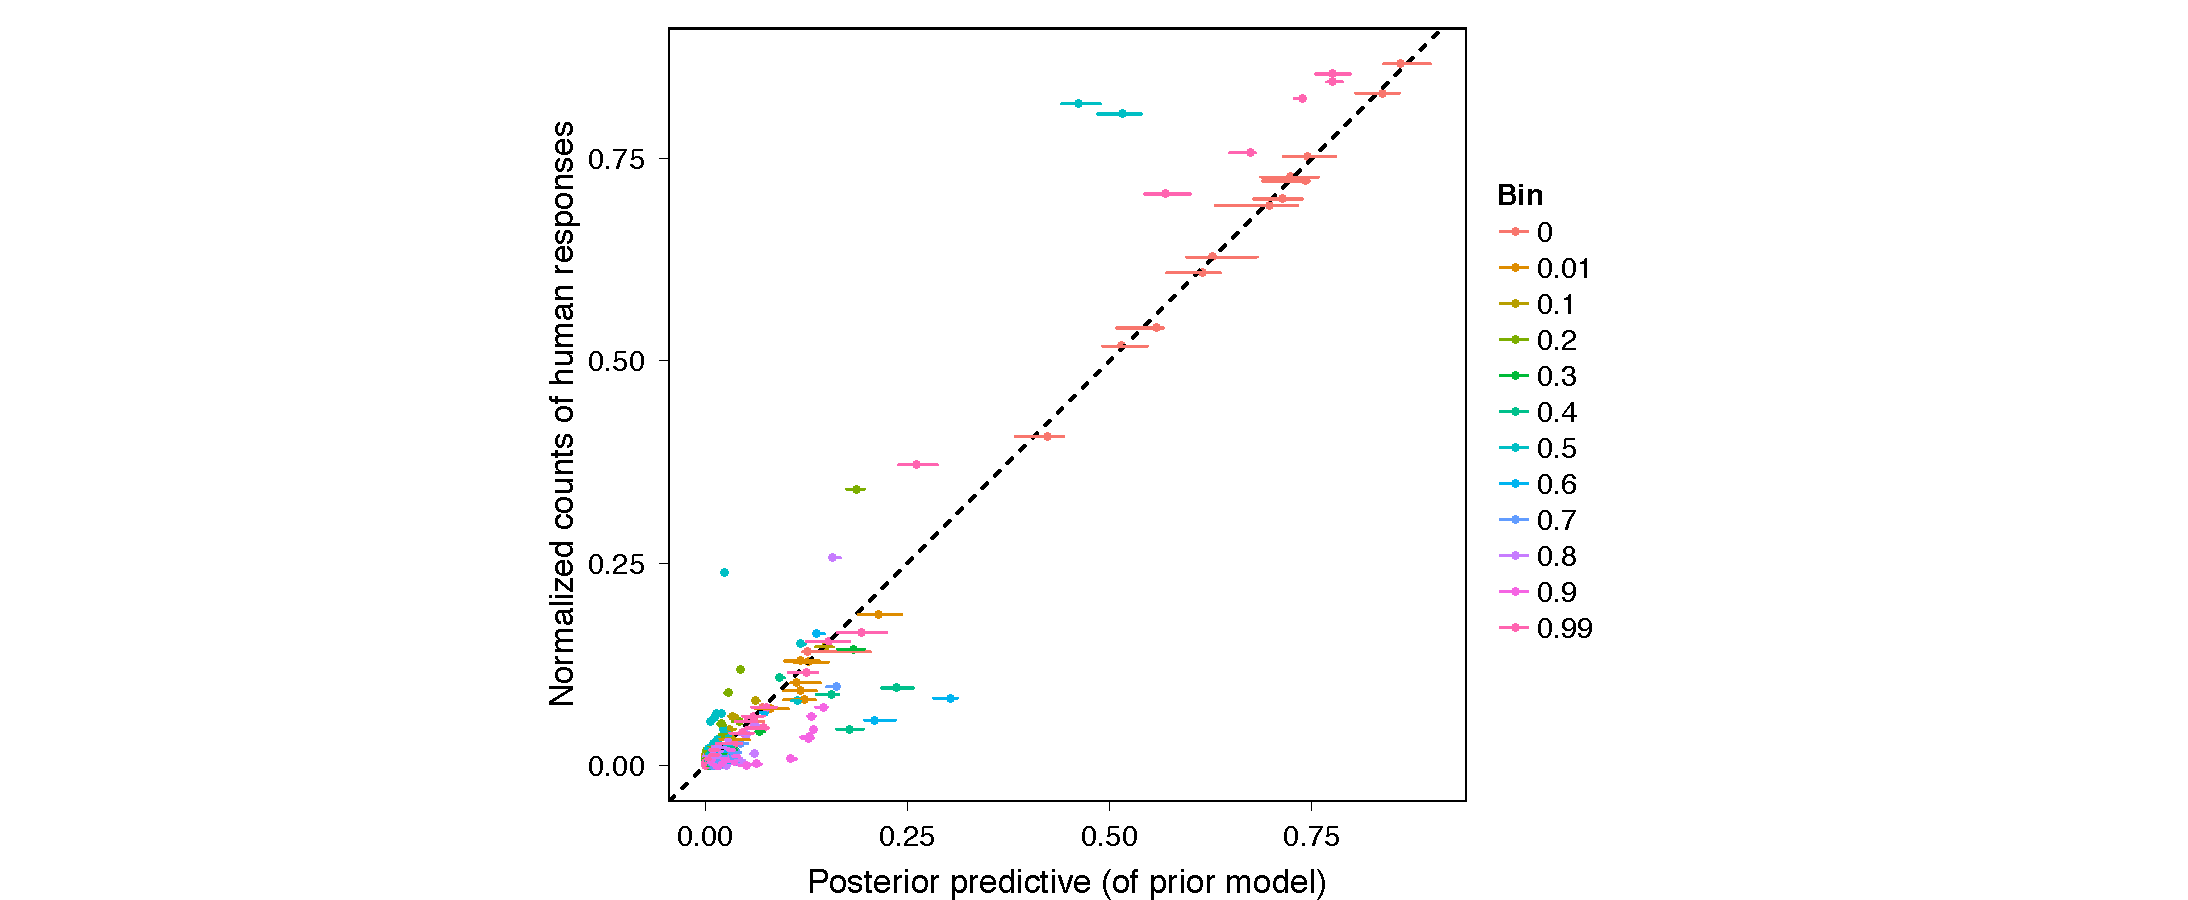
\includegraphics[width=0.6\columnwidth]{postPred-priorModel.pdf}
    \caption{Posterior predictive distribution of the structured, statistical model thought to give rise to the human data in the prior elicitation task. The close alignment between model and data suggests the assumption of a structured prior is warranted.}
  \label{fig:pp-priorModel}
\end{figure}

\subsection*{Results}

Using this structure, we can explore our twenty-one properties:
Figure \ref{fig:priors1a} shows the estimated mixture-parameter $\theta$ (the potential of the property to be present in a kind) and the mean prevalence when the property is present, $\gamma$. 
We see significant diversity among these properties in both dimensions, resulting in priors over prevalence with dramatically different shapes (insets). 
This diversity matters because the model predictions for generic interpretation and felicity depend on the shape of the prior distribution (insets show example $L_1$ interpretation posteriors).
Lowering $\theta$ effectively makes the property more distinctive by increasing the relative probability mass at 0\%; this relaxes the truth conditions by making a lower threshold more informative.\mht{Make a comment how $\theta$ is not the same as cue-validity?}.
Increasing $\gamma$ means the property is expected to be present in more members of the category; this tends to make truth conditions stricter, by reducing the range of prevalence values higher than the prior expectation. 

%
\begin{figure*}
%\floatbox[{\capbeside\thisfloatsetup{capbesideposition={right,top},capbesidewidth=4cm}}]{figure}[\FBwidth]
%{\caption{A test figure with its caption side by side}\label{fig:test}}
\centering
    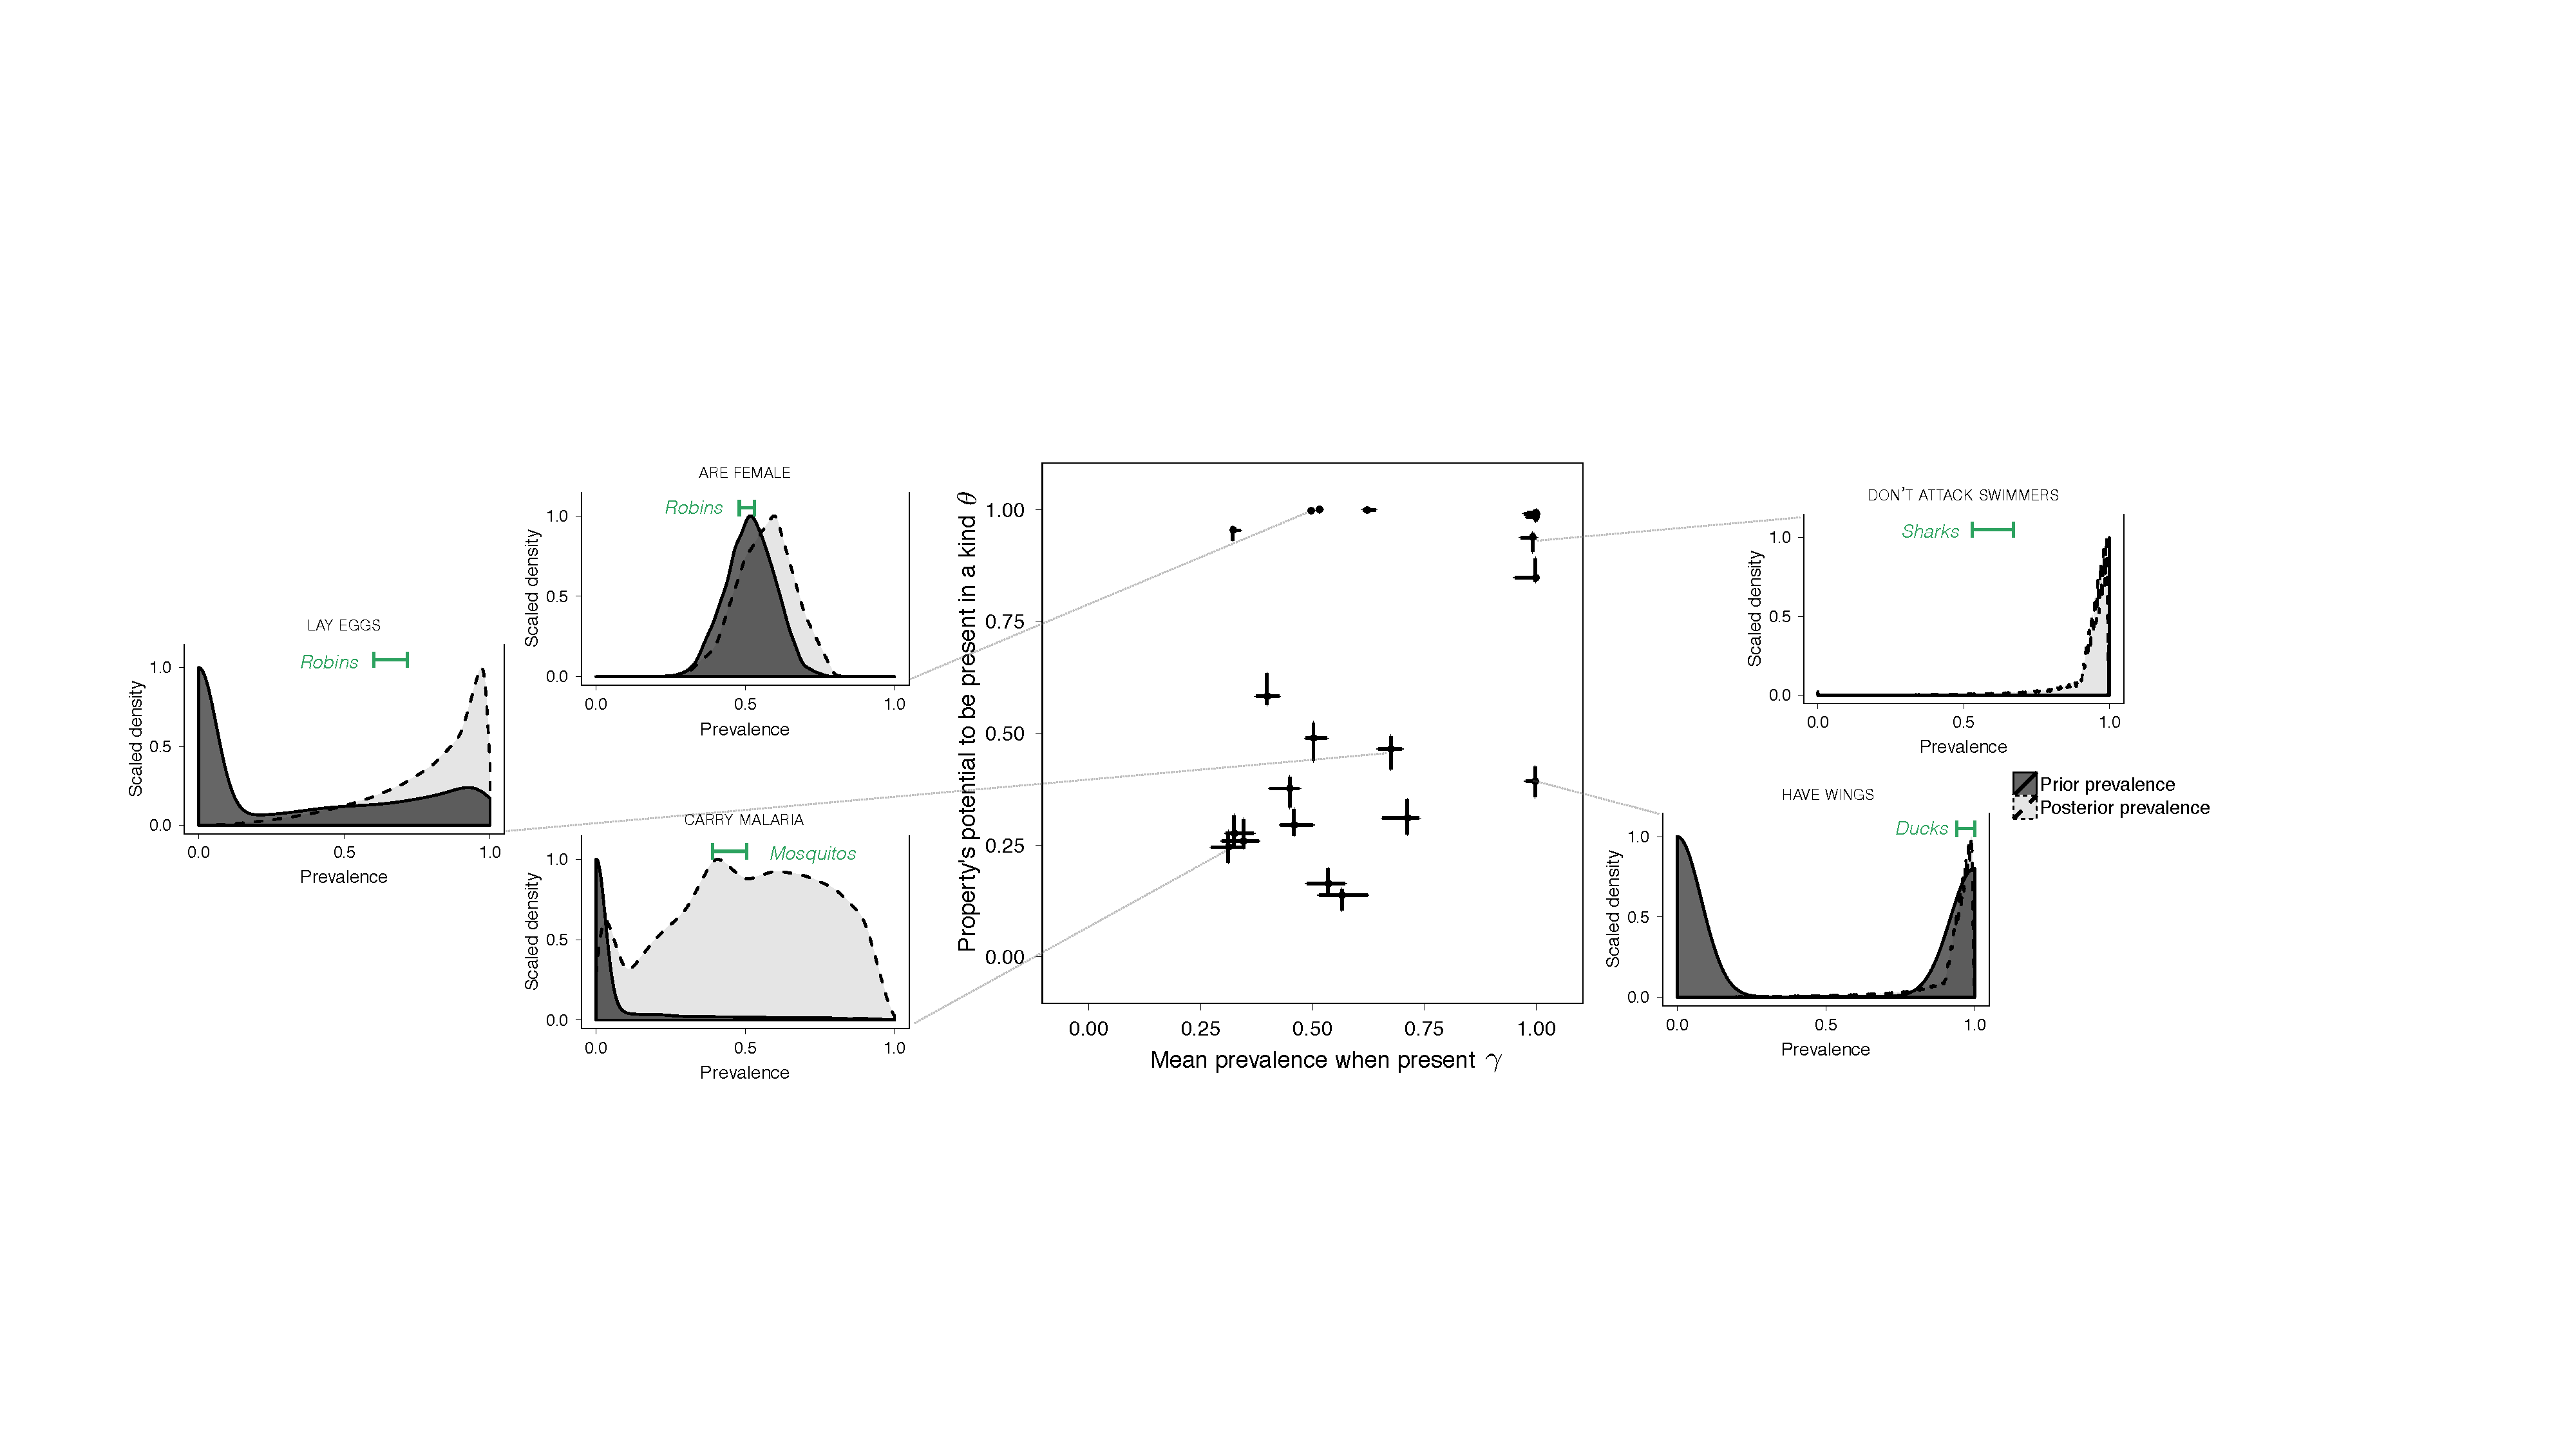
\includegraphics[width=\columnwidth]{prevalence-scatter-wDists_wide.pdf}
    \caption{Prevalence prior distributions empirically elicited for twenty-one animal properties.
    Prior distributions are summarized by $\theta$----a property's potential to be present in a category----and $\gamma$----the mean prevalence when it is possible for the property to be present in a category.
    Inset plots display example empirical prior distributions over prevalence together with corresponding $L_1$ model predictions: the posterior after hearing a generic utterance. 
    Intervals on the top of plots show human beliefs about the prevalence of the property within a target category.
%    Posterior distributions show what happens to a listener's belief about the prevalence after hearing the associated generic. 
    Felicitous generic utterances result when the target prevalence is more likely under the posterior than under the prior.
 %   \ndg{should mark the observed within-category prevalence for target kinds in pop-outs? or maybe one of the axes of main plot should be that?}
     Error bars denote 95\% Bayesian credible intervals (same for Figure \ref{fig:prior2}).
    }
  \label{fig:priors1a}
\end{figure*}

Using these priors, we can explore what prevalence a listener would be likely to be infer upon hearing a generic using $P_{L_{1}}(x , \tau \mid u)$ (Figure \ref{fig:priors1a} insets). 
Here, the corresponding prior beliefs, $P(x)$, can also be interpreted as the posteriors upon hearing the null utterance, because the null utterance has no information content.
We see the interpretation of the generic is quite variable in our empirically derived priors.
For instance, in the case of \textsc{carries malaria}, the prior is very left-skewed; here, the threshold $\tau$ can plausibly be quite low while still being informative, since a low threshold still rules out many possible alternative kinds (and their corresponding degree of prevalence).
Properties like \textsc{doesn't attack swimmers} are very right-skewed; here, even a relatively high threshold would not result in an informative utterance (as not many kinds would be ruled out), and so the generic is unlikely to be used by speaker $S_2$ unless the property is practically-universal within the target category. 
Some properties have priors that are unimodal with low variance (e.g. \textsc{is female}); these properties are present in every kind in almost exactly the same proportion and thus are too obvious and certain to allow for an informative generic utterance: The posterior is not very different from the prior. 
We are now in a position to explore the quantitative predictions of truth judgments using the $S_2$ model.

\section*{Experiment 1b: Truth judgments of familiar generics}


We tested the degree to which the $S_2$ model, Eq.~\ref{eq:S2}, coupled with the empirically-elicited prevalence priors from Expt.~1a predicted that a given category--property pair (e.g. \textsc{robins} and \textsc{lays eggs}) would result in a felicitous generic (e.g. \emph{Robins lay eggs.}). 


\subsection*{Method}

\subsubsection*{Participants}

We recruited 100 participants over MTurk. 
We chose this number of participants based on intuition from similar experiments which were designed primarily to test a quantitative model.
Participants were restricted to those with US IP addresses and with at least a 95\% MTurk work approval rating. 
4 participants were excluded for failing to pass a catch trial.
5 participants self-reported a native language other than English; removing their data has no effect on the results reported. 
The experiment took about 3 minutes and participants were compensated \$0.35.


\subsubsection*{Procedure and materials}

Participants were shown thirty generic sentences in bare plural form one after another. 
They were asked to press one of two buttons to signify whether they agreed or disagreed with the sentence (see {\it SI Table 2} for complete list and {\it SI Section B} for more details). 
%\ndg{the order was randomized between particiapants?}
The thirty sentences were presented in a random order between participants and covered a range of conceptual categories: Characteristic (e.g. \emph{Ducks have wings.}), Minority (e.g. \emph{Robins lay eggs.}), Striking (e.g. \emph{Mosquitos carry malaria.}), False generalization (e.g. \emph{Robins are female.}), and False (e.g. \emph{Lions lay eggs.}).
We also aimed to include generics that were both acceptable and unacceptable with low, medium, and high prevalence.
Approximately 10 true, 10 false, and 10 uncertain truth-value generics were selected.


As a manipulation check, participants were asked at the end of the trials which button corresponded to ``Agree''. 4 participants were excluded for failing this trial.


\subsection*{Data analysis and results}
 
 As a manipulation check, the first author assigned an \emph{a priori} truth-judgment (true/false/indeterminate) to each stimulus item.
This was a significant predictor of the empirical truth judgments: true generics were significantly more likely to be agreed with than the indeterminate generics ($\beta = 3.14; SE = 0.15; z = 21.5$), as revealed by a mixed-effect logistic regression with random by-participant effects of intercept.
Indeterminate generics were agreed with \emph{less} likely than chance ($\beta = -0.49; SE = 0.09; z = -5.3$) but significantly more than false generics ($\beta = 2.09; SE = 0.14; z = 14.5$).

 
 
 %Does subjective belief about the prevalence of the property within the target kind predict the felicity of a generic utterance?
From the prevalence-prior data (Expt.~1a) we can estimate participants' beliefs about the prevalence of a property \emph{for a given kind} (e.g.~the percentage of \textsc{robins} that \textsc{lay eggs}; see green intervals on Figure \ref{fig:priors1a} and \emph{SI Table 2}).
% for Maximum A-Posteriori (MAP) estimates and 95\% Bayesian Highest Density Intervals (HDI) over the mean prevalence for each property--category pairing). %We first compare the predictions of Eq.~\ref{eq:S2} to 
As a simple baseline hypothesis, we first explore whether these prevalence values themselves predict generic endorsement (e.g.~does the fraction of \textsc{robins} that \textsc{lay eggs} predict the felicity of \emph{Robins lay eggs}?).
A little over half of the variance in truth judgments data is explained by the prevalence of the property within the kind alone ($r^2 = 0.599$; MSE=0.065; \emph{SI Figure 2}). 
This is not surprising given our inclusion of high-prevalence true generics (e.g. \emph{Leopards have spots.}) and low-prevalence false generics (e.g. \emph{Leopards have wings.}). 
However, large deviations remain from an account based purely on target-category prevalence: Generics in which the target category has intermediate prevalence (prevalence quartiles 2 and 3: $ 20\% < prevalence < 64\%$), are not at all explained by prevalence within those categories ($r_{Q2,3}^2 = 0.029$; MSE = 0.110).


\mht{Add null model of cue validity?}

The speaker model, $S_2$ in Eq.~\ref{eq:S2}, predicts an endorsement probability for a generic sentence, given prior beliefs for the property and a target prevalence. 
We use the estimated within--kind prevalence as the target prevalence that speaker $S_2$ is trying to communicate, and use the
empirically inferred priors from Expt.~1a. The model has one remaining parameter: the speaker optimality parameter $\lambda$ (in Eq.~\ref{eq:S1}).

For data analysis, we put an uninformative prior over this parameter, with a range consistent with previous literature using the same model class.

$$
\lambda \sim \text{Uniform}(0,20)
$$

To learn about the \emph{a posteriori} credible values of our model parameter, we collected 3 MCMC chains of 100,000 iterations removing the first 50,000 iterations, using the Metropolis-Hastings algorithm. 
The 95\% Highest Probability Density (HPD) Interval for the speaker rationality parameter is [3.36, 4.98], consistent with previous literature using the same model class \mht{Add parameter posteriors to appendix}.

We evaluate the model by examining the posterior predictive distribution of responses. 
The posterior predictive distribution marginalizes over the inferred parameter values to produce predictions about what the data should look like given the pragmatics model and the observed data. 
This is akin to fitting the parameters and is an important step in model validation: It shows what data is actually predicted by the model. 
As we see in Figure \ref{fig:modeldataBars}, the pragmatic speaker model $S_2$, using empirically measured priors, does a very good job of explaining human truth judgments ($r^2=0.981$; MSE=0.003; Figure \ref{fig:modeldataBars}). 
Generics that received definitive agreement or disagreement are predicted to be judged as such by the model (corners of Figure \ref{fig:modeldataBars}), including items for which target-category prevalence is not a good indicator of the acceptability (for prevalence quartiles 2 and 3, $r_{Q2,3}^2=0.955$; MSE=0.005; Figure \ref{fig:modeldataBars}, intermediate shades).

Thus, we see the probabilistic pragmatics model explains the truth judgments when the prevalence alone does not and for a diverse range of generic statements.
Our model explains the puzzling flexibility of generic truth-conditions as the result of communicative pressures (\emph{be truthful}, \emph{be informative}) operating over diverse prior beliefs about the properties. 
 

%\begin{figure}
%\centering
%    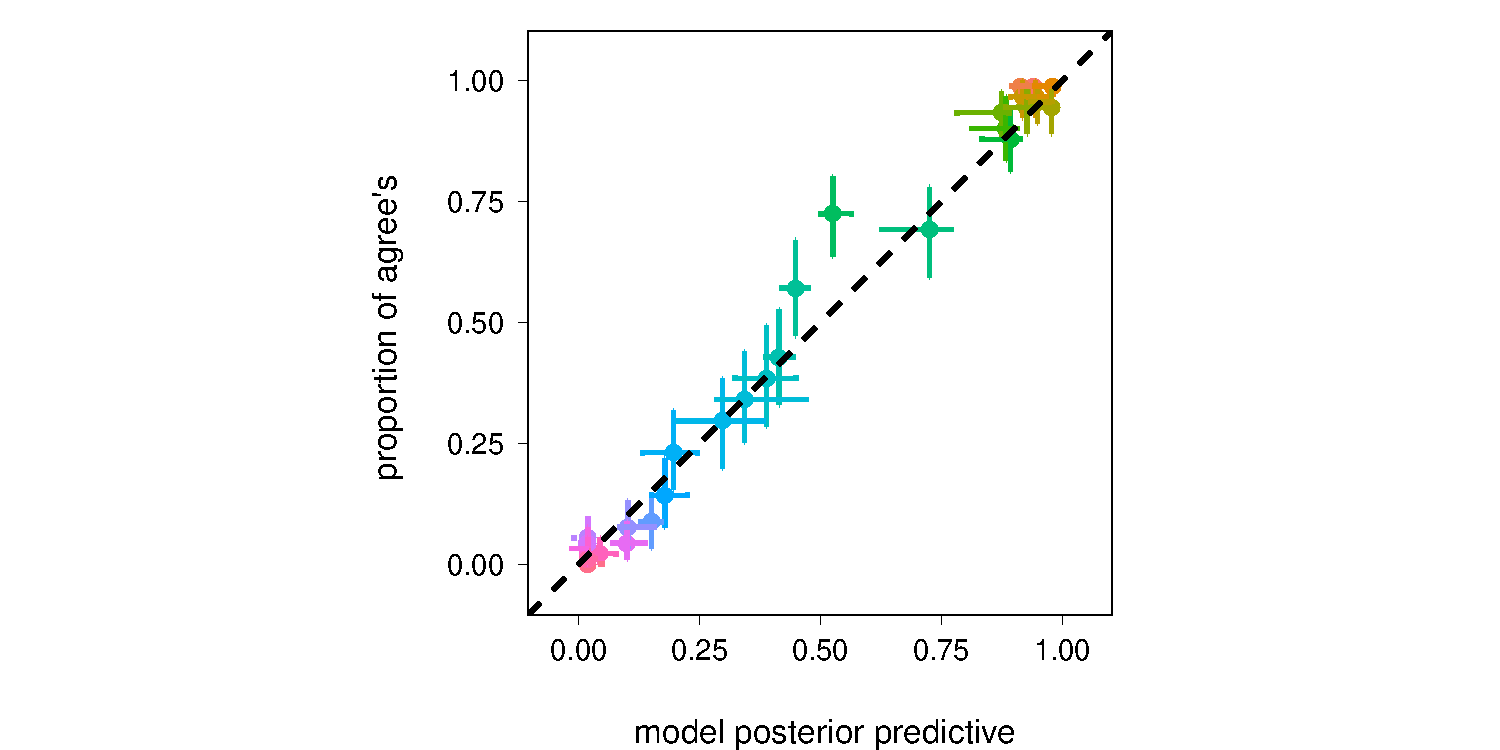
\includegraphics[width=\columnwidth]{tj_n100_tjVsPostpred_95hdi.pdf}
%    \caption{Truth judgments from Expt.~1b for each item vs. the posterior predictive MAP estimates for the target item using the lifted-threshold model with the empirical priors elicited in Expt.~1a. Color spectrum corresponds to the rank ordering of the truth judgment data; similarly colored dots received similar truth judgments. Error bars correspond with 95\% bootstrapped confidence intervals for the participant data and 95\% highest probability intervals for the model predictions.}
%  \label{fig:modeldataScatter}
%\end{figure}


%Participants were restricted to those with US IP addresses and with at least a 95\% MTurk work approval rating. 
%4 participants were excluded for failing to pass a catch trial.
%5 participants self-reported a native language other than English; removing their data has no effect on the results reported. 
%The experiment took about 3 minutes and participants were compensated \$0.35.
%Participants were asked to report whether they agreed or disagreed with generic sentences presented in bare plural form. 
%Items were presented sequentially, and participants reported whether or not they agreed with the sentence by pressing either \textsc{p} or \textsc{q} (randomized between-subjects). 
%Generic sentences were selected to correspond with the properties used in Expt.~1a. 
%Approximately 10 true, 10 false, and 10 uncertain truth-value generics were selected (see {\it SI Table 2} for full list of items).
%As a manipulation check, participants were asked at the end of the trials which button corresponded to ``Agree''. 
%4 participants were excluded for failing this trial.
%

%\ndg{maybe one more sentence about the desired range of variation: from true to false and in between, but also true with low prevalence, etc...?}
%
%The 30 generic sentences fell into 3 \emph{a priori} categories: definitely true, definitely false, and neither true nor false (Figure \ref{fig:modeldataBars}, light bars). 

%%the manipulation check here doesn't add much... moved to supplement...
%As a manipulation check, the \emph{a priori} truth-judgment we assigned was a significant predictor of the empirical truth judgments: true generics were significantly more likely to be agreed with than the indeterminate generics ($\beta = 3.14; SE = 0.15; z = 21.5$), as revealed by a mixed-effect logistic regression with random by-participant effects of intercept.
%Indeterminate generics were agreed with \emph{less} likely than chance ($\beta = -0.49; SE = 0.09; z = -5.3$) but significantly more than false generics ($\beta = 2.09; SE = 0.14; z = 14.5$).


%The probabilisitic model of generic production is fully specified by Eqs.~\ref{eq:L1} -- \ref{eq:S2}, the empirically-elicited $P(x)$, and the speaker rationality parameter $\lambda$ in Eq.~\ref{eq:S1}. 
%Because $\lambda$ is not of theoretical interest here, it is marginalized according to Bayesian data analysis principles \cite{LW2014}. 
% $P(x)$ describes the belief distribution on the prevalence of a given property (e.g. \textsc{lay eggs}) across relevant categories. 
% This distribution, which is conceivably very different for different properties, is common-sense background knowledge. 
% We measure it empirically by asking participants ($n=57$) about the prevalence of our target properties for many different animal categories\footnote{Our experiments stay within the animal kingdom because we expect there to be considerably less variability in participants beliefs about animals than about other types of categories (e.g. social categories)}. 
% 
%, which is crucial since this drives variance in model predictions.


%for four example properties---there are substantial differences between different types of properties. 
%\ndg{how about being more specific about what we mean by between and within category (mass on zero; mean of remaining mass?). say the model suggests these are important. make a plot showing these for all our properties..?}

%The property ``lays eggs'' is relatively rare across categories (large density at 0); even when some animals within a category have manes, there is considerable variation of the percent that do, though the expected value is around 67\% (Figure \ref{fig:priors1a} bottom left; within-category prevalence given by blue dotted line). 
%By contrast, the distribution over ``is male'' has a lot less diffuse: the property is highly prevalent across categories (almost no mass at 0), and within a category it is present in about 50\% of cases.
%The property ``has wings'' is not particularly rare across categories (probably owing to the fact that bird categories are heavily represented in our stimulus set), and within a category is widespread, as reflected by the bimodal distribution. 
%Finally, ``has malaria'' is an example of a property that is both rare across-categories and within-categories. 
%The property is absent from most animal species, and even when it is present, it is only present in a small number of cases.





%\begin{figure*}
%\centering
%\begin{minipage}[b]{.49\textwidth}
%    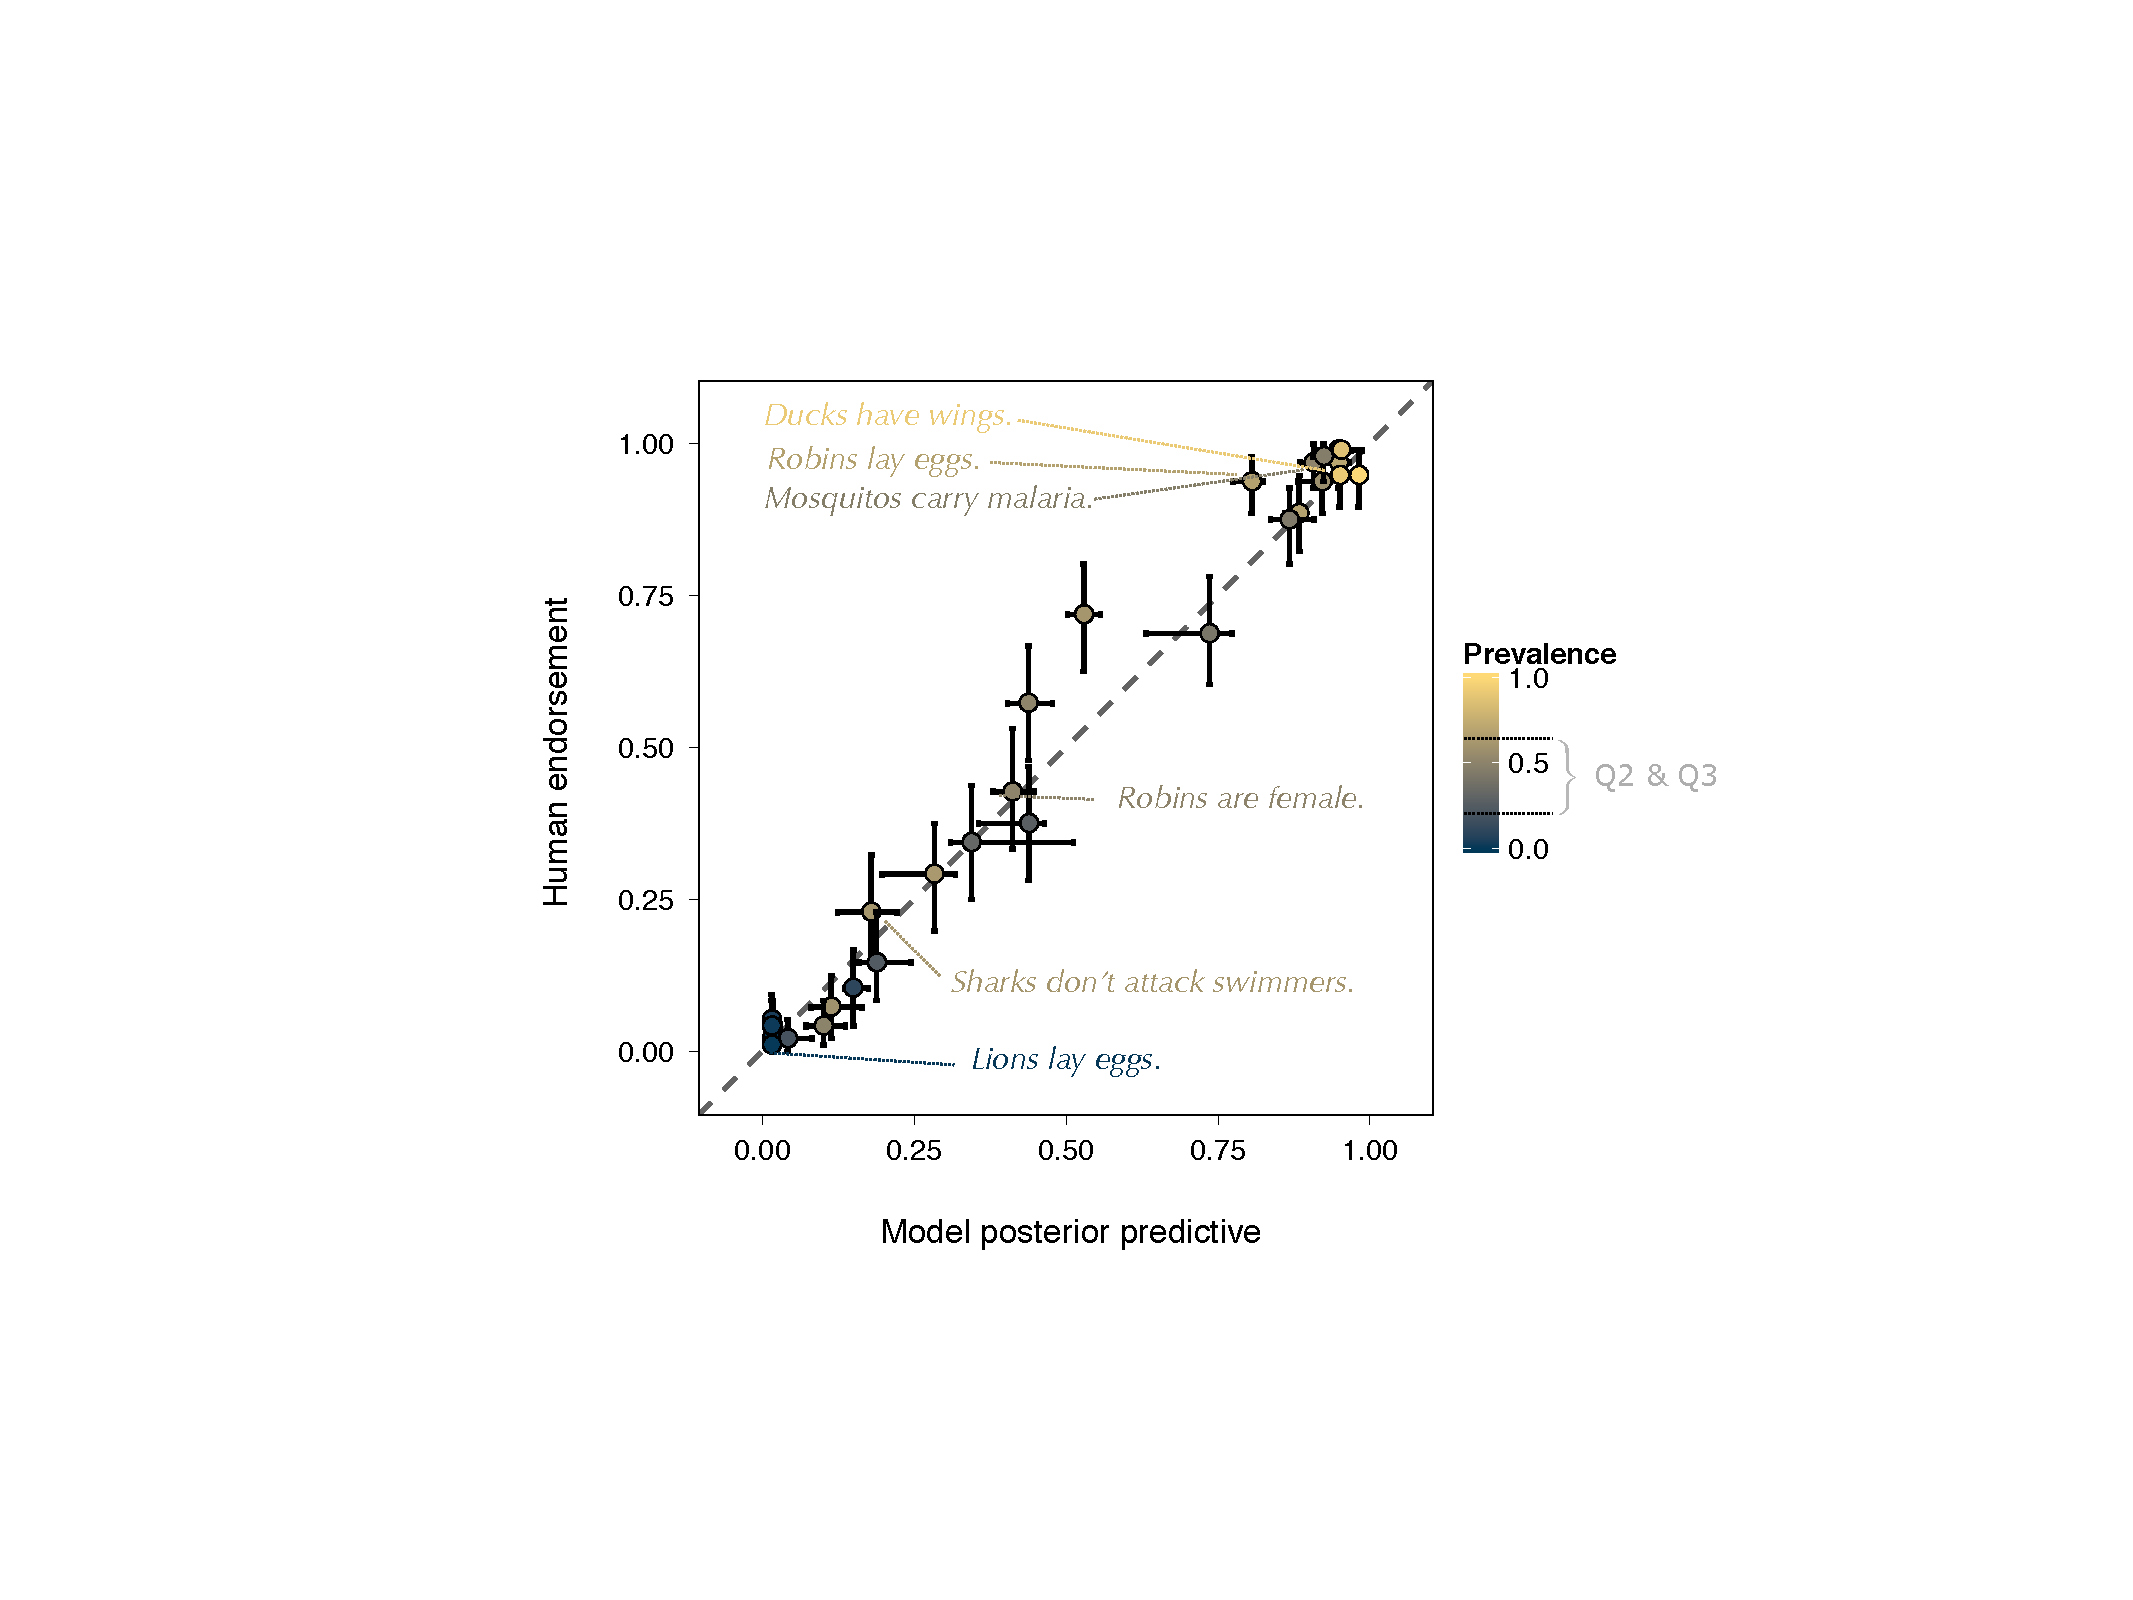
\includegraphics[width=8.7cm]{truthjudge-scatter-wLabels.pdf}
%    \caption{Human acceptability judgments and model predictions for thirty generic utterances about familiar animals and properties. 
%    Color denotes target-category prevalence of the property, with darker colors indicating lower prevalence. 
%    Intermediate prevalences (quartiles 2 \& 3) are in intermediate shades (marked on color bar).
%    Error bars correspond with 95\% bootstrapped confidence intervals for the participant data and 95\% highest probability intervals for the model predictions.
%    }
%  %\label{fig:modeldataBars}
%\end{minipage}
%\begin{minipage}[b]{.49\textwidth}
%\centering
%    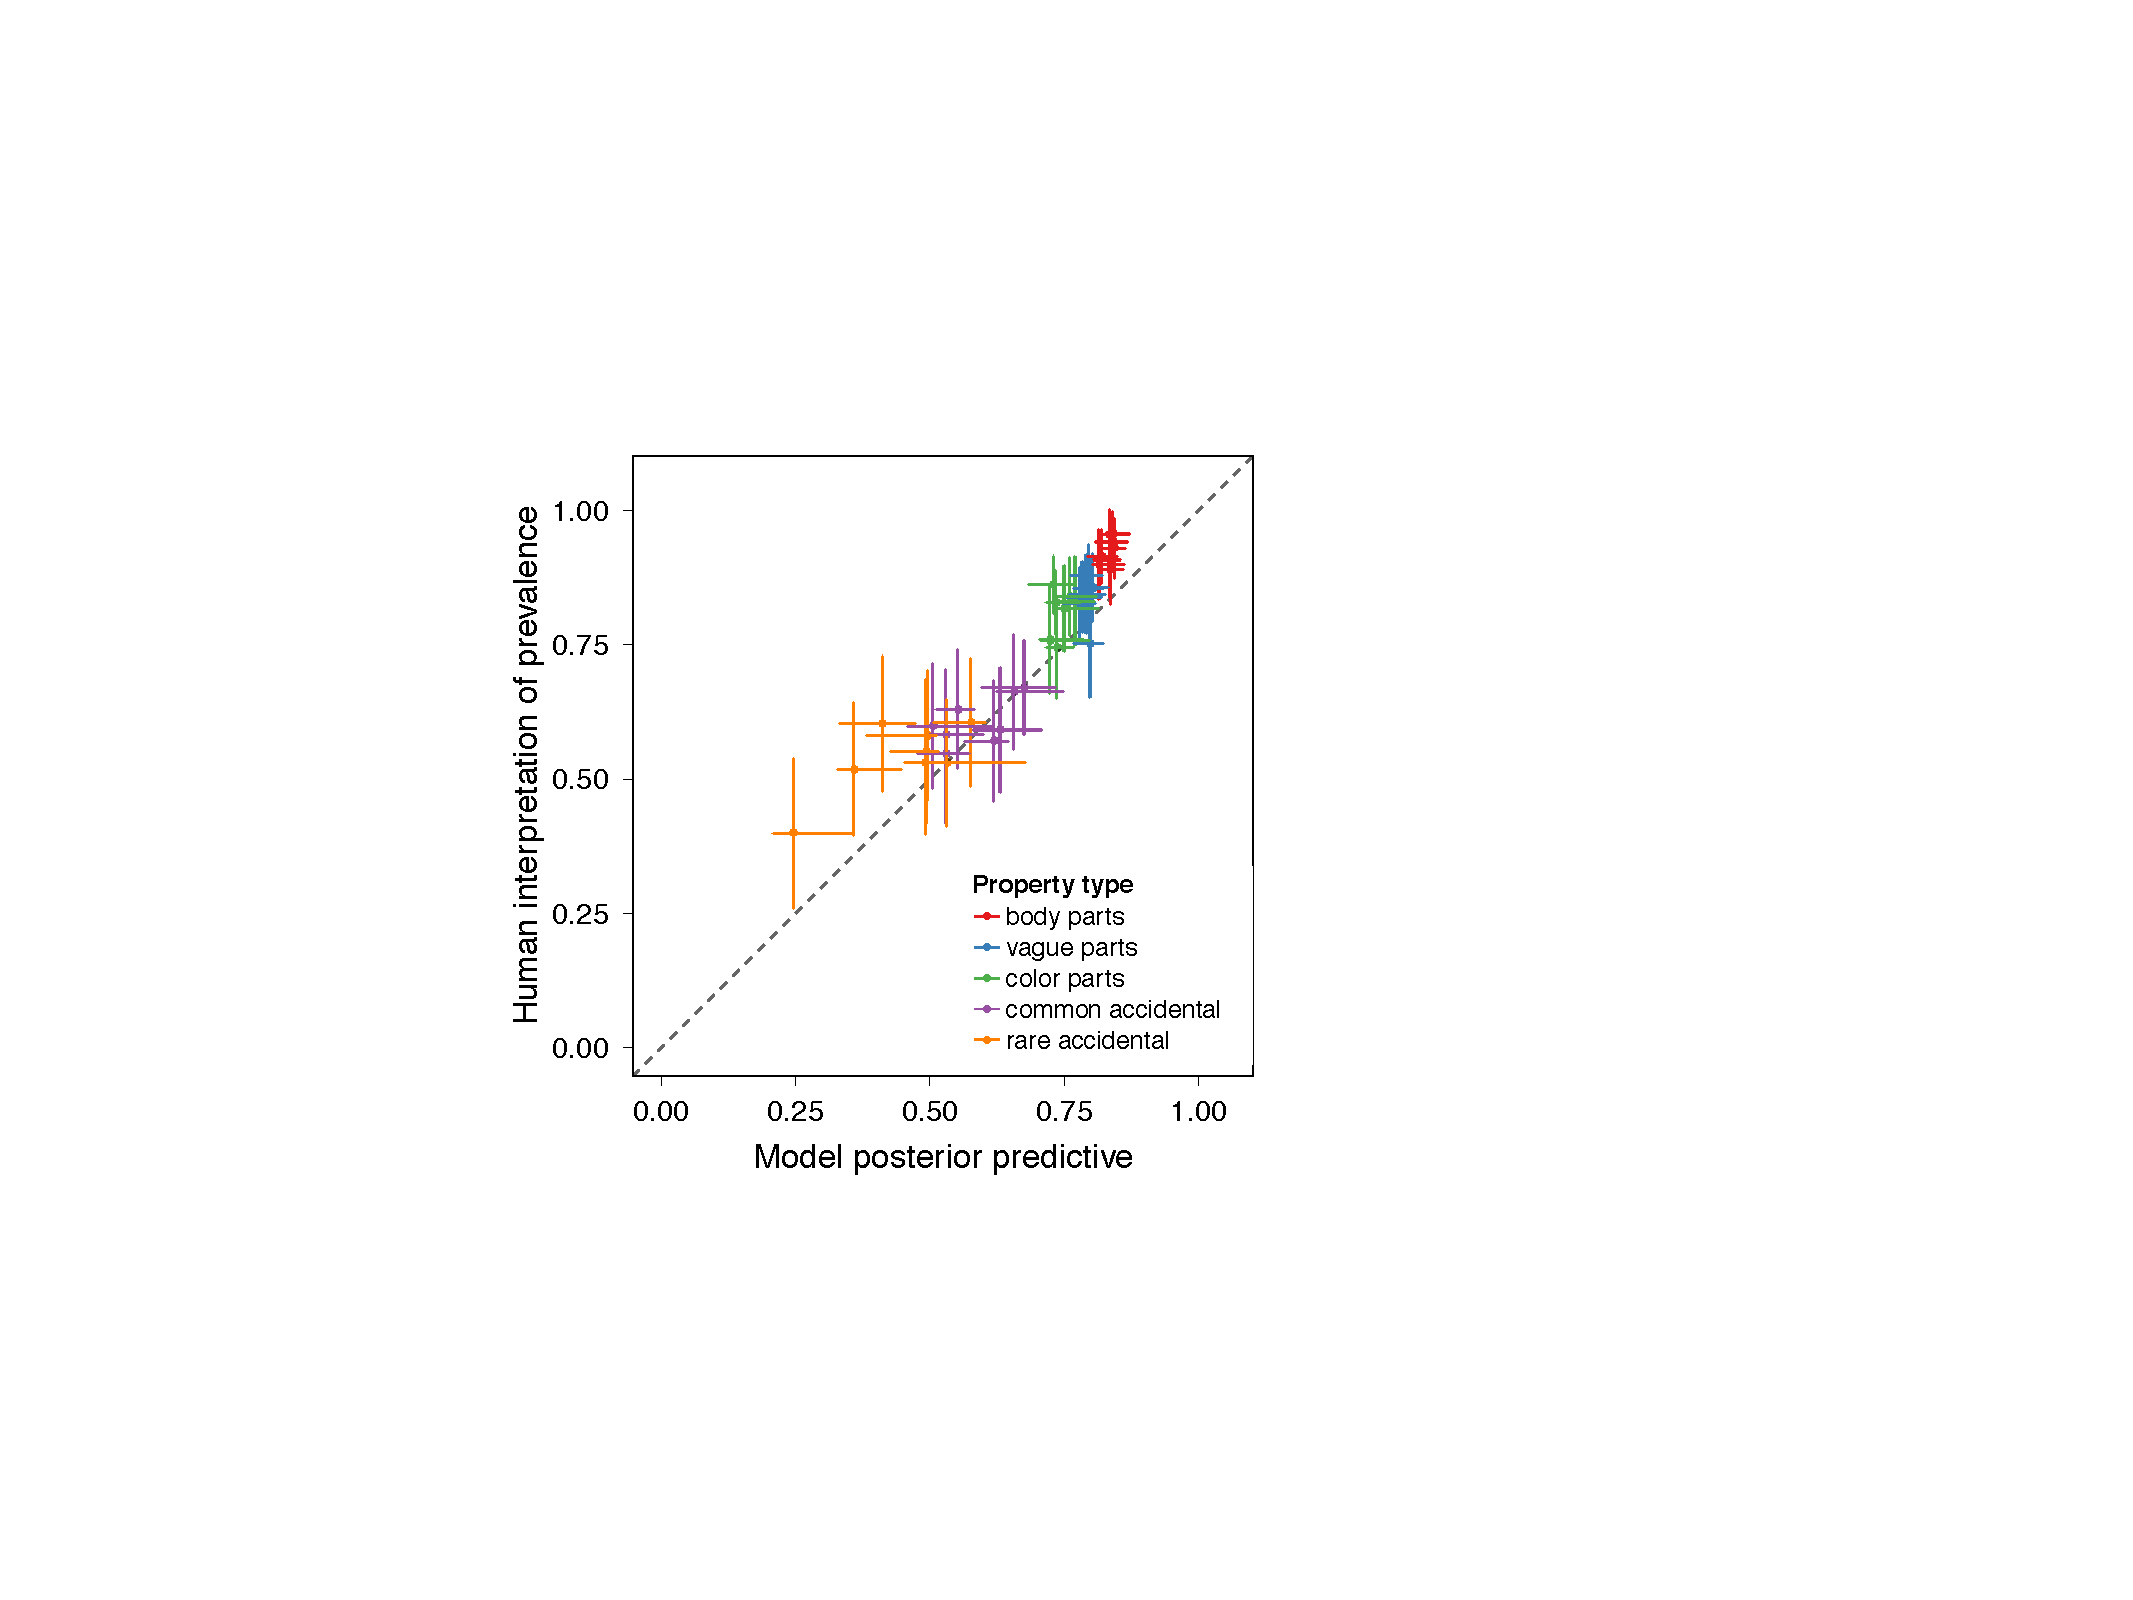
\includegraphics[width=6.7cm]{implied-byItem-mh100kX2b.pdf}
%    \caption{Human interpretation of prevalence upon hearing a generic compared with the $L_1$ model posterior predictive. 
%    Participants display graded endorsements of generics in terms of prevalence based on type of property (which is also associated with \emph{mean prevalence when present} $\gamma$, see Figure 3).
%    The model displays the same variability of interpretation, producing strong interpretations for generics of biological properties (red, blue, green) and weaker interpretations of generics of accidental properties (purple, orange).
%        Error bars denote bootstrapped 95\% confidence intervals for the data and Bayesian 95\% credible intervals for the model.}
% % \label{fig:impliedByItem}
%\end{minipage}
%\end{figure*}

\begin{figure}
\centering
    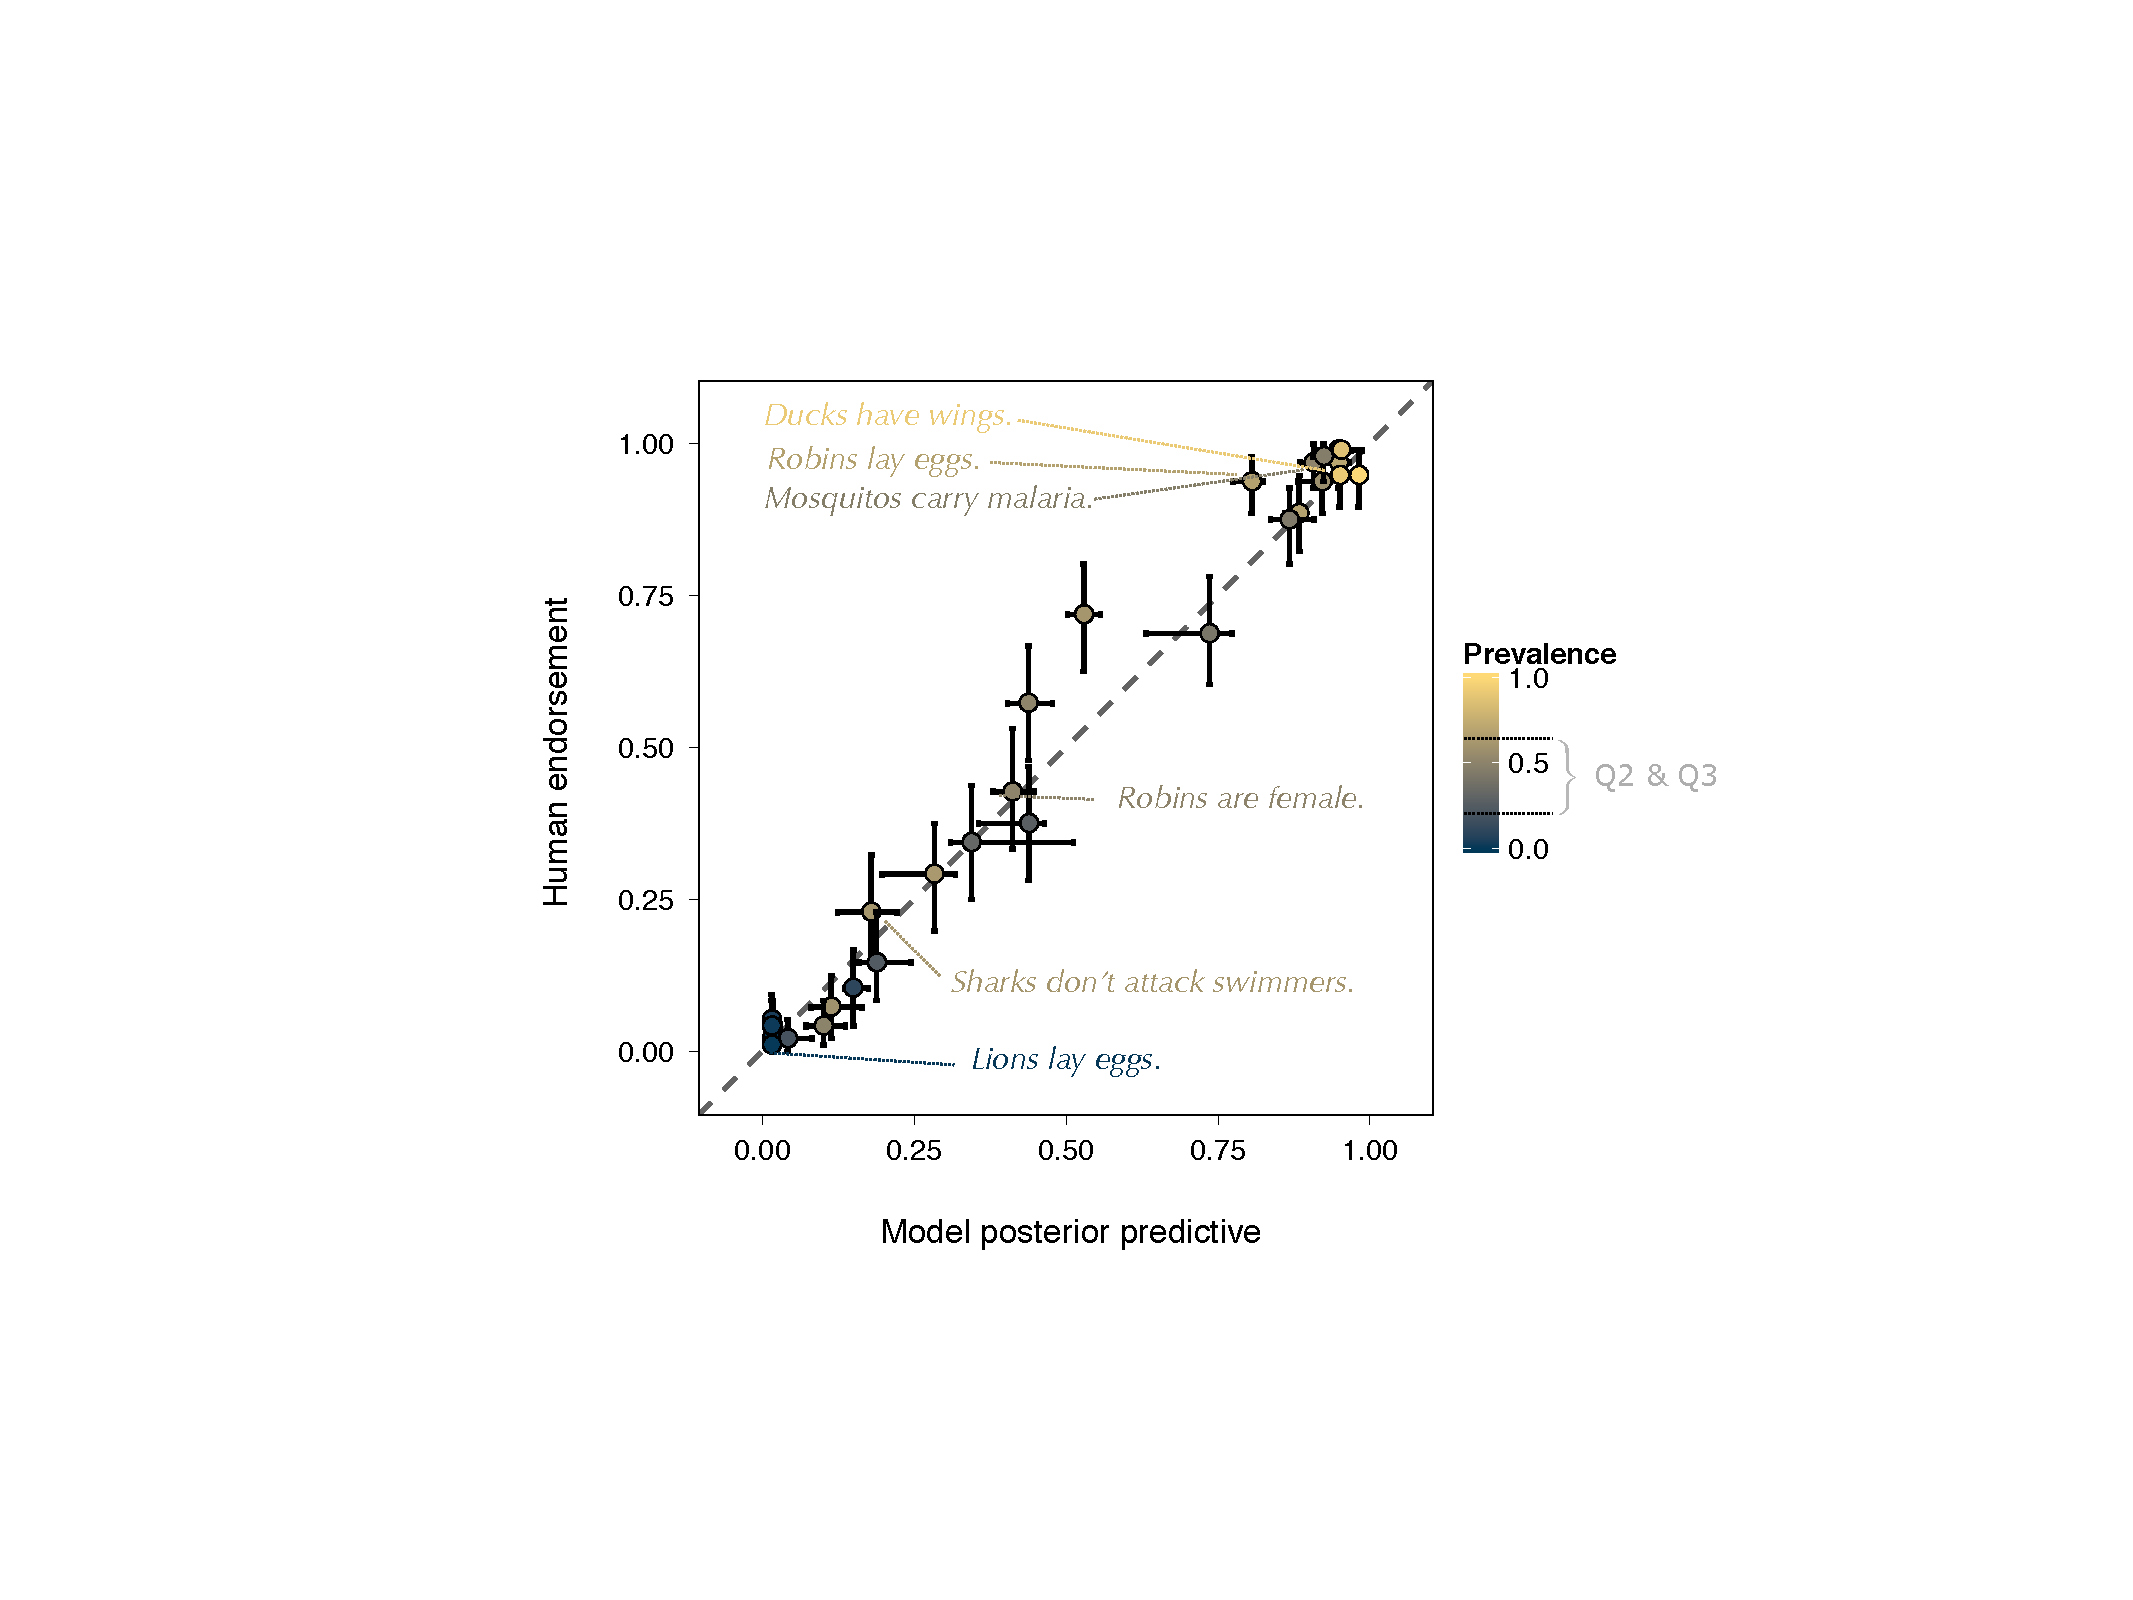
\includegraphics[width=0.7\columnwidth]{truthjudge-scatter-wLabels.pdf}
    \caption{Human acceptability judgments and model predictions for thirty generic utterances about familiar animals and properties. 
    Color denotes target-category prevalence of the property, with darker colors indicating lower prevalence. 
    Intermediate prevalences (quartiles 2 \& 3) are in intermediate shades (marked on color bar).
    Error bars correspond with 95\% bootstrapped confidence intervals for the participant data and 95\% highest probability intervals for the model predictions (same for Figures \ref{fig:impliedByItem} and \ref{fig:exp2b}).
    }
  \label{fig:modeldataBars}
%\end{minipage}
%\begin{minipage}[b]{.49\textwidth}
%\centering
%    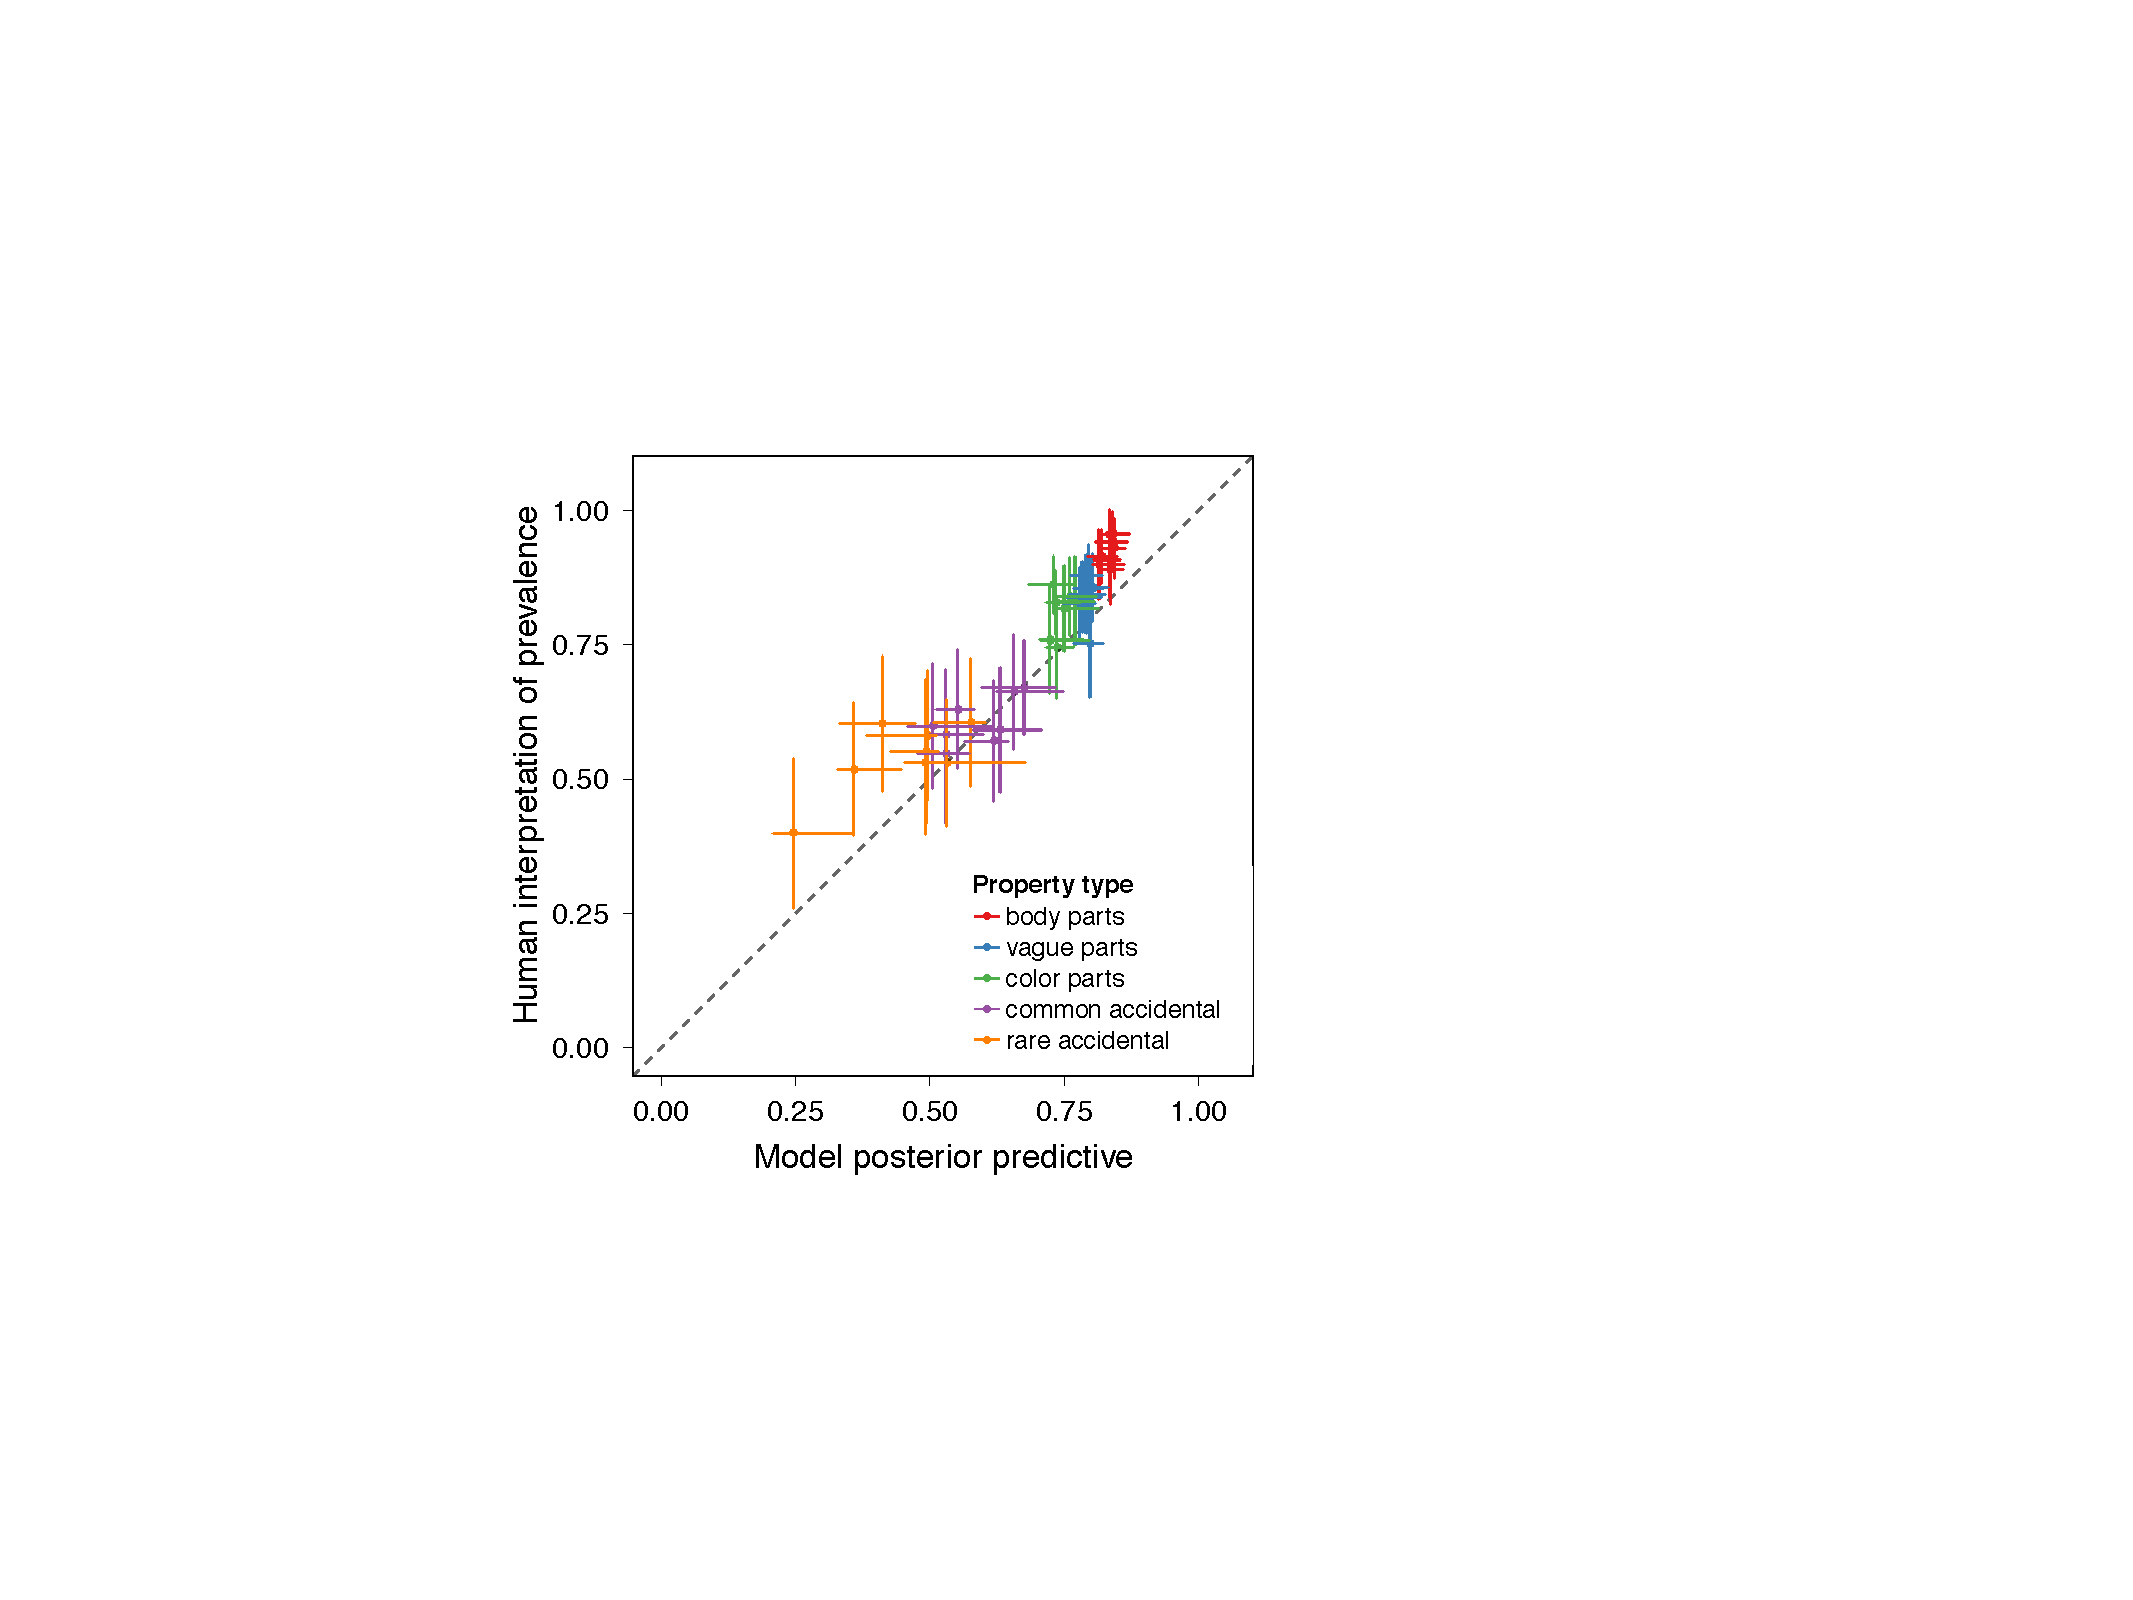
\includegraphics[width=6.7cm]{implied-byItem-mh100kX2b.pdf}
%    \caption{Human interpretation of prevalence upon hearing a generic compared with the $L_1$ model posterior predictive. 
%    Participants display graded endorsements of generics in terms of prevalence based on type of property (which is also associated with \emph{mean prevalence when present} $\gamma$, see Figure 3).
%    The model displays the same variability of interpretation, producing strong interpretations for generics of biological properties (red, blue, green) and weaker interpretations of generics of accidental properties (purple, orange).
%        Error bars denote bootstrapped 95\% confidence intervals for the data and Bayesian 95\% credible intervals for the model.}
% % \label{fig:impliedByItem}
%\end{minipage}
\end{figure}


\section*{Strong interpretations for novel categories}


One of the most important roles for generic language is to provide learners information about new or poorly understood categories. 
This role depends on how unfamiliar generic sentences are interpreted \cite<e.g.>{Gelman2002, Cimpian2010}.
The pragmatic theory we present includes such a theory of generic comprehension: the listener model (Eq.~\ref{eq:L1}) describes interpretation of a generic utterance---\emph{Feps \textsc{have property}}---without previously knowing the prevalence of the property within this kind.
With an uncertain meaning and the pressure to be informative, interpretation in the theory is heavily driven by \emph{a priori} beliefs about properties. 
Classic work in generalization suggests beliefs about the prevalence of properties differ by type of property, including relatively fine distinctions among properties that are all biological in nature \cite{Nisbett1983}. 
We leverage these strong but diverse expectations, using forty different properties to explore a wide range of \emph{a priori} beliefs about prevalence. 
These items make up four categories of properties: body parts of a particular color (e.g. \textsc{has green feathers}), described vaguely (e.g. \textsc{has small wings}), in accidental or disease states (e.g. \textsc{has wet fur}, \textsc{has swollen ears}), and without modification (e.g. \textsc{has claws}).

We first use a novel method for measuring \emph{a priori} beliefs about the prevalence of these properties (Expt.~2a). We then test the predictions of the pragmatic listener model $L_1$ using these empirically derived priors against human \emph{interpretations} of novel generic sentences (Expt.~2b). We also explain a previously reported empirical asymmetry between truth conditions and interpretations by comparing the speaker $S_2$ and listener $L_1$ models in the same experimental context (Expt.~2c).


\section*{Experiment 2a: Prevalence priors for unfamiliar categories}

To measure the prior over prevalence using \emph{familiar} categories (Expt. 1a), participants filled out a table with rows corresponding to different animal kinds and columns corresponding to different properties.
We cannot do the same for unfamiliar kinds: Nothing would distinguish the rows.
% (What percentage of feps have yellow fur?)
%But without reference to a familiar kind, how can one know what prevalence to expect? 
We instead leverage the latent structure uncovered in Expt.~1a, where we decomposed prevalence priors into 2 components: the property's potential to be present in a kind and the mean prevalence when present.
This suggests a two-stage elicitation procedure.
%
% we discovered a latent structure to the prevalence priors task.
%A simple, structured Bayesian model easily accommodated the data using two components: the property's potential to be present in a kind and the expected prevalence when present.
%We leveraged this structure to measure prevalence priors with unfamiliar categories. 


%, structuring our task into questions about the property's potential to be present in a kind and the expected prevalence when present; we then used a Bayesian statistical model to reconstruct the underlying prior distribution. 
%
%
%
%Pilot testing suggested this was a pragmatically strange setup when using novel kinds: answering ``What percentage of lorches have green feathers?'', when participants knew nothing about lorches, was difficult.


\subsection*{Method}

\subsubsection*{Participants}

We recruited 40 participants over MTurk.  
We again chose this number of participants based on intuition from similar experiments which were designed primarily to test a quantitative model.
Participants were restricted to those with US IP addresses and with at least a 95\% MTurk work approval rating. 
All participants were native English speakers. 
The experiment took about 5-7 minutes and participants were compensated \$0.75.

\subsubsection*{Procedure and materials}

%Classic work in generalization suggests beliefs about the prevalence of properties differ by type of property, including relatively fine distinctions between properties that are all biological in nature \cite{Nisbett1983}. 
We constructed forty different properties to explore a wide range of \emph{a priori} beliefs about prevalence. 
These items make up four categories of properties: body parts of a particular color (e.g. \textsc{has green feathers}), described vaguely (e.g. \textsc{has small wings}), in accidental or disease states (e.g. \textsc{has wet fur}, \textsc{has swollen ears}), and without modification (e.g. \textsc{has claws}).
%\footnote{The distinction between common and rare accidental properties was determined empirically by analyzing the data by item, and performing a median split based on the \emph{a priori} mean prevalence when present, $\gamma$, of the property.}.
%We are interested in testing in the predictive power of 
Because pilot testing revealed more variability for items in the accidental category relative to the other types of properties, we used twice as many exemplars of accidental properties, yielding a more thorough test of the quantitative predictive power of the $L_1$ interpretation model. 
We used 8 exemplars of each of the three non-accidental properties (``parts'', ``colored parts'', ``vague parts''), and 16 exemplars of accidental properties, building on a stimulus set from \citeA{Cimpian2010}.
All materials are shown in Table S3.

Participants were introduced to a data-collection robot that was tasked with learning about properties of animals. 
Participants were told the robot randomly sampled an animal to ask the participant about (e.g. The robots says: ``We recently discovered animals called feps.''). 
The robot then asks the participant two questions, aimed to measure the two components of the structured prior model: (1) the potential of the property to be present in a kind and (2) the expected prevalence when present.
To get at (1), the robot asked how likely it was that ``there was \emph{a} fep with \textsc{property}'' (potential to be present), to which participants reported on a scale from ``unlikely'' to ``likely''.
For example, it is very likely that there is a fep that is female, less likely that there is a fep that has wings, and even less likely that there is a fep that has purple wings. 
To get at (2), the robot then asked, ``Suppose there is a fep that has wings. What percentage of feps do you think have wings?'' (expected prevalence when present). 
Participants completed a practice trial to make sure they understood the meanings of these two questions.

%responded using slider bars for each question.
%
%$P(x)$ was measured empirically ($n=40$, {\it Experiment 2a}), and the most likely priors were inferred using the same structured, statistical approach used for the familiar generics experiment.

\subsection*{Data analysis and results}

We used the same structured, statistical model from Expt.~1a.
The only difference from Expt.~1a. is that our experimental data comes from inquiring about the parameters of the priors directly, as opposed to asking about particular samples from the prior (i.e. particular kinds) as was done in Expt.~1a. 
%For Expt.~2a, participants are asked questions directly targeting $\theta$ and $\gamma$ in the above model (see {\it Expt. 2a}).
We assume these two measurements follow Beta distributions ($d_{potential} \sim \text{Beta}(\gamma_{1}, \xi_{1})$; $
d_{expected} \sim \text{Beta}(\gamma_{2}, \xi_{2})$), and construct single prevalence distributions, $P(x)$, by sampling from the posterior predictive distribution of prevalence as we did before: $P(x) = \int [ \theta\cdot \text{Beta} (x \mid \gamma_{2}, \xi_{2}) + (1 -  \theta) \cdot \delta_{x=0} ] \cdot \text{Beta}(\theta \mid \gamma_{1}, \xi_{1}) d\theta$.
We used the same priors over parameters $\theta, \gamma_{i}, \xi_{i}$ as in Expt.~1a.
%
%\begin{minipage}{0.5 \textwidth} \small
%\begin{align*}
%%\end{align*}
%%%\end{minipage}
%%%
%%To %\begin{minipage}{0.5 \textwidth} \small
%%%        \begin{align*}
%%\theta & \sim \text{Beta}(\gamma_{potential}, \xi_{potential}) \\ 
%P(x) = [ \theta\cdot \text{Beta} (x \mid \gamma_{2}, \xi_{2}) + (1 -  \theta) \cdot \delta_{x=0} ] \cdot \text{Beta}(\theta \mid \gamma_{1}, \xi_{1})
%%
%%\begin{cases} 
%%		\text{Beta}(\gamma_{expected}, \xi_{expected}) &\mbox{if } \text{Bernoulli}(\theta) = \textsc{t} \\
%%				\delta_{x=0} &\mbox{if } \text{Bernoulli}(\theta) = \textsc{f} \\
%%		\end{cases} \\
%\end{align*}
%%\ndg{this eqn is kind of ugly. simplify in coordination with the earlier one?}
%
%%	 P(d_{observed} ) = \theta \cdot \beta(\gamma,\xi)+ (1 - \theta) \cdot \delta_{d=0} 


Figure \ref{fig:prior2} shows a summary of the elicited priors, in terms of the diversity of $d_{potential}$ and $d_{expected}$.
Biological properties are expected to be \emph{a priori} more prevalent within a kind when present than accidental properties, with additional fine-grained differences within biological and accidental properties.
Like the priors elicited using familiar categories, these priors elicited using unfamiliar categories have diverse shapes (see insets). 
Biological properties (``biological'', ``vague'', and ``color'' body parts) have prevalence distributions that are bimodal with peaks at 0\% and near-100\% prevalence. 
Interpretations of generics about these properties ($L_1$ model, Eq.~\ref{eq:L1}) update these distribution to concave posteriors peaked at 100\% (Figure \ref{fig:prior2}; red, blue and green insets); the model predicts these novel generics will be interpreted as implying the property is widespread in the category \cite{Gelman2002}.
By contrast, accidental properties (both ``rare'' and ``common'') follow unimodal prior distributions and update to convex posterior distributions, predicting weaker and more variable interpretations of novel generics for these properties \cite{Cimpian2010c}. 
%These convex posteriors show that generics about accidental or temporary properties come with highly uncertain interpretations, plausibly as a consequence of theory-driven considerations \cite{Cimpian2010c}. 


\begin{figure*}
\centering
    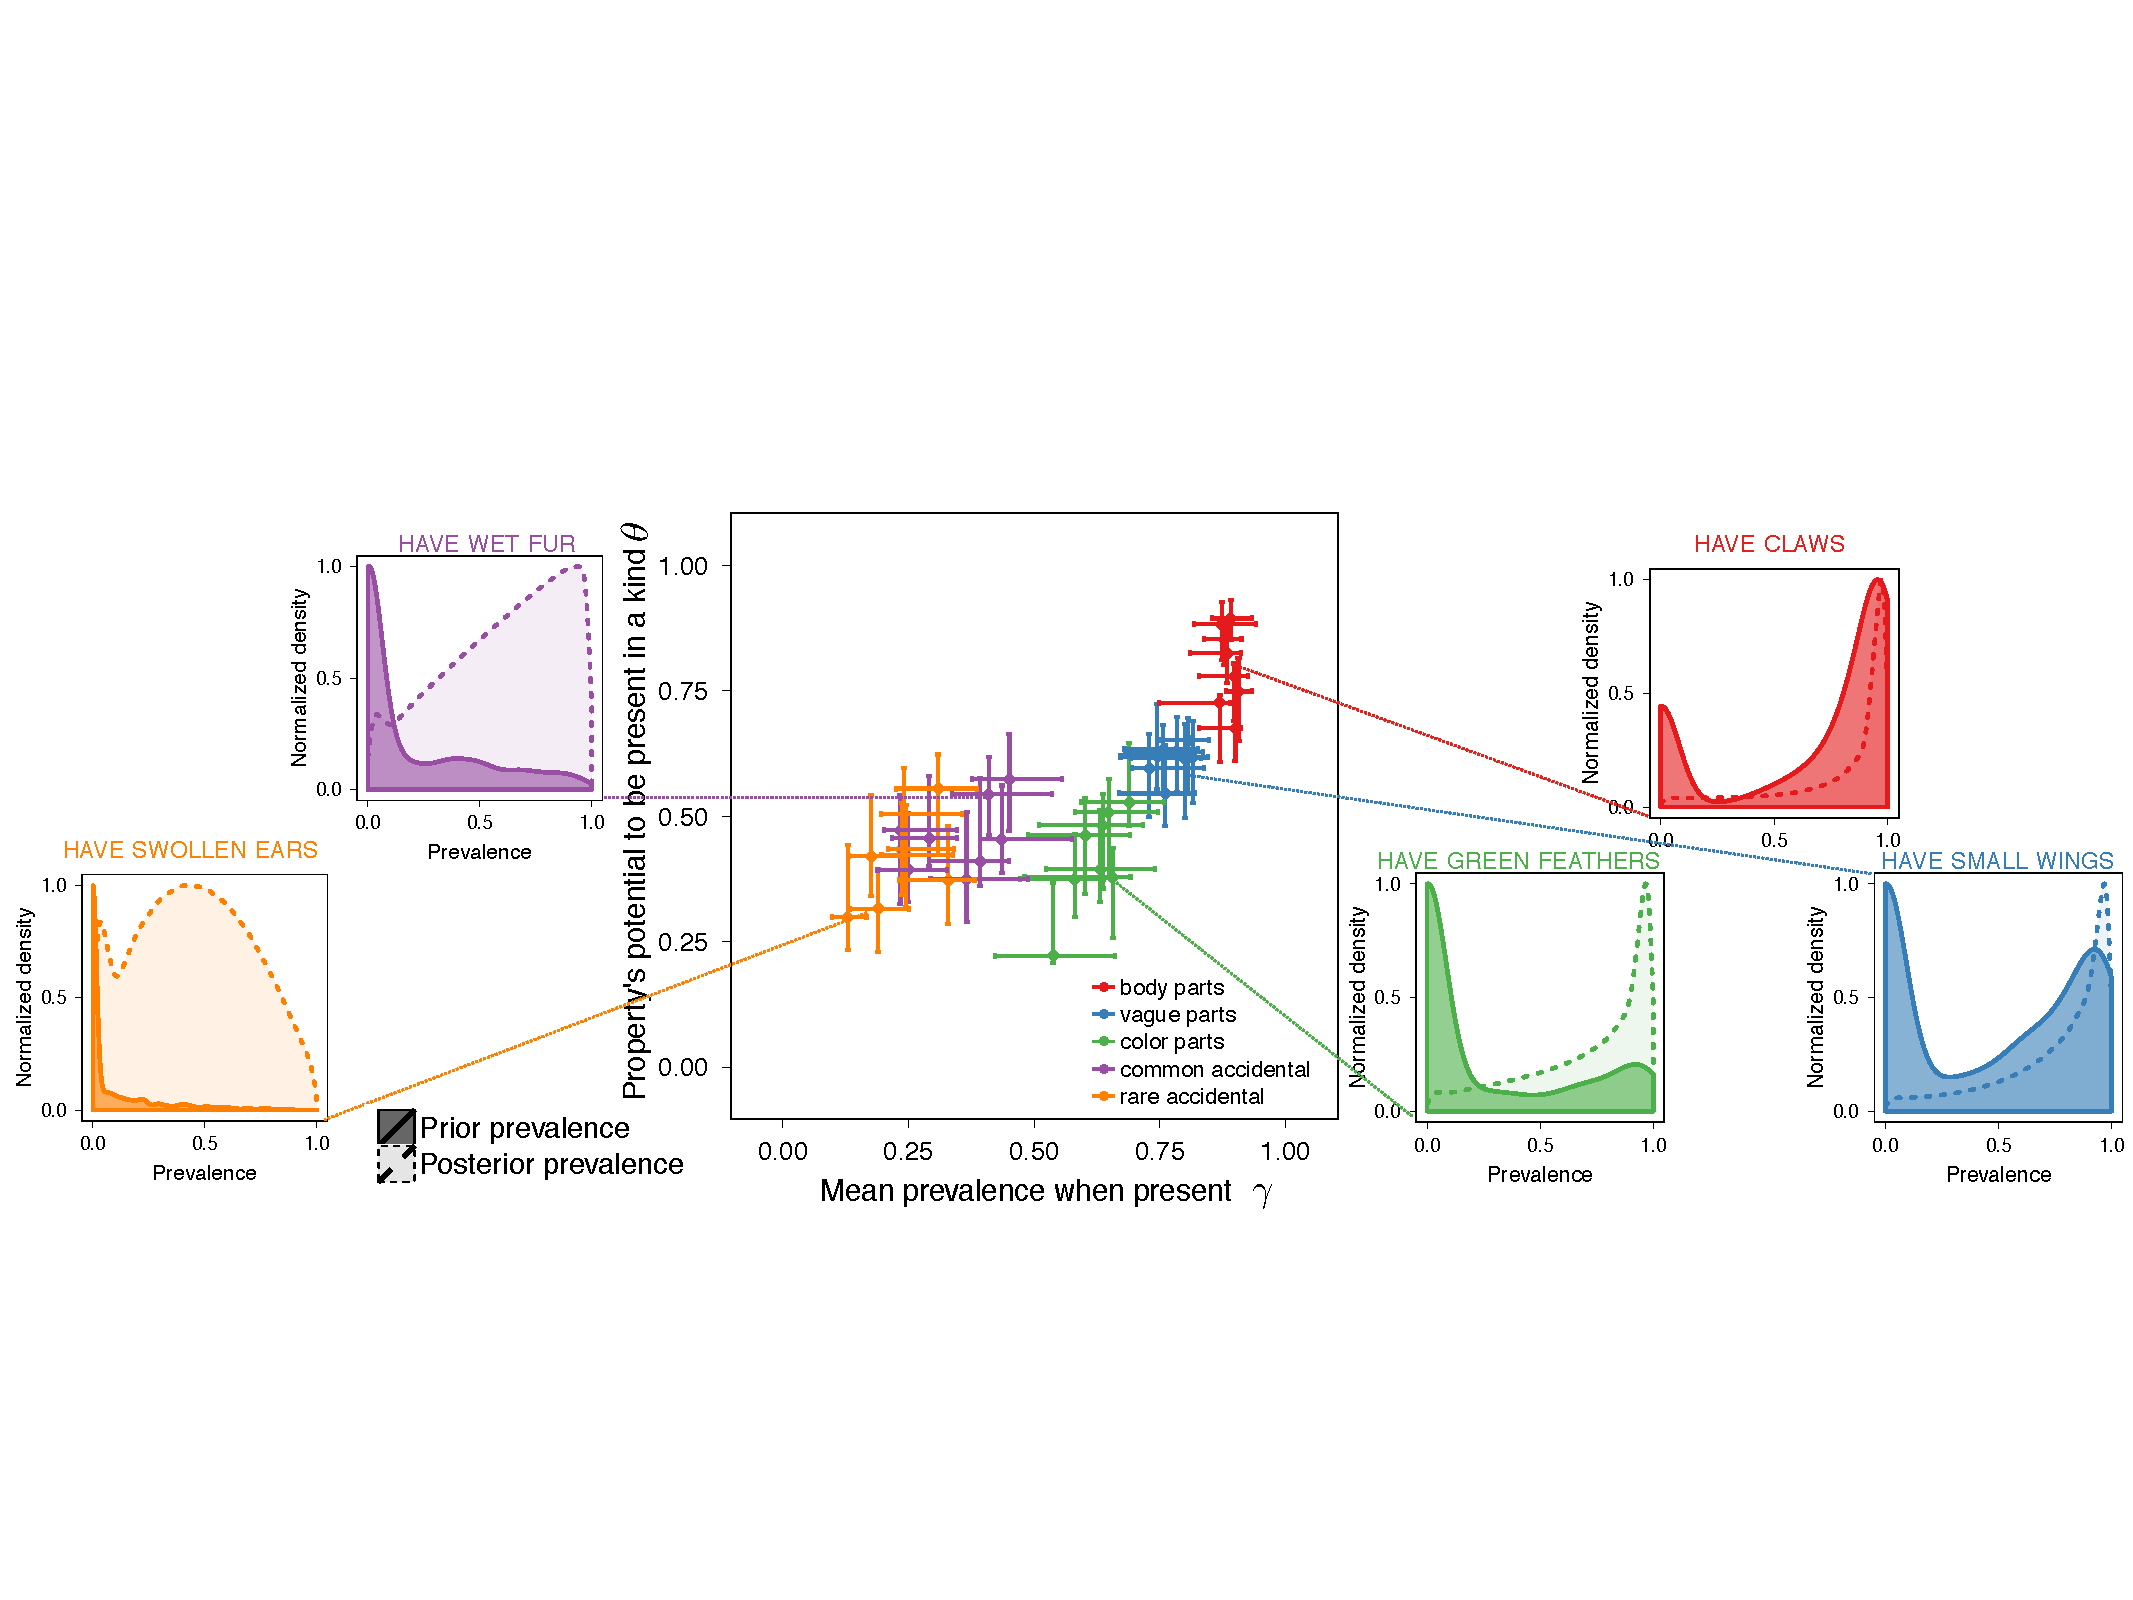
\includegraphics[width=\columnwidth]{prevalence-asymmetry-scatterwDists-byItem3.pdf}
    \caption{Prevalence prior distributions empirically elicited for 40 animal properties.
    Parameters of the structured statistical model---$\theta$ and $\gamma$---reveal quantitative differences in beliefs about the prevalence of conceptually different types of properties (scatterplot). 
    Inset plots show differences in shapes between biological properties (red, green, blue; bimodal) and accidental properties (orange, purple; unimodal).   
  These differences give rise to the variability of interpretations of generic utterances. 
  %    Error bars denote Bayesian 95\% credible intervals.
  }
  \label{fig:prior2}
\end{figure*}




\section*{Experiment 2b: Interpretations of novel generics}

The pragmatic listener model $L_1$ (Eq.~\ref{eq:L1}) predicts that the interpretations of generics in terms of prevalence should vary as a function of the prevalence prior.
Here, we test the degree to which the predictions based on the empirically elicited prevalence priors for 40 items (from Expt.~2a) match human judgments of how the widespread the property is upon hearing a generic.

%We tested the degree to which the $L_1$ listener model, Eq.~\ref{eq:L1}, coupled with the empirically-elicited priors, $P(x)$, from Expt.~2a predicted the interpretation of a generic sentence consisting of a novel category with one of the forty properties described above.
%degree to which the generic implied the property was widespread in the kind. 

%The full cover story is described in {\it SI Section C} and is the same for Expt.~2c.
%The original study by \citeauthor{Cimpian2010} found a difference in the implied prevalence between ``color parts'' (e.g. \textsc{yellow fur}) and accidental properties (e.g. \textsc{wet fur}).
%The prevalence priors inferred from Expt.~2a suggest that generic interpretation could be even more variable.
%For this reason, we included three types of biological properties: parts (e.g. \textsc{fur}), color--part pairs (e.g. \textsc{yellow fur}) and gradable adjective--part pairs (e.g. \textsc{curly fur}). 
%We also coded the accidental properties from Expt.~2a as either ``common'' or ``rare'' using a by-item median split based on \emph{a priori} expected prevalence when present.
%Most of the materials we used were from \citeauthor{Cimpian2010}. 
%The materials used were 30 novel animal categories (e.g. lorches, morseths, blins) each paired with a unique property. 
%Biological properties were made by pairing a color with a body-part (e.g. purple feathers, orange tails). 
%Accidental properties used the same set of body-parts but modified it with an adjective describing an accidental or disease state (e.g. broken legs, wet fur). 
%Each participant saw a random subset of 10 unique animal-property pairs for each type of property (biological and accidental). 


\subsection*{Method}

\subsubsection*{Participants}

We recruited 40 participants over MTurk to determine how widespread different properties are believed to be upon hearing a novel generic.  
The experimental design is very similar to \citeA{Cimpian2010}, and we chose to have a sample size at least twice as large as the original study (original n=15). 
This is a quantitative experiment with only quantitative comparisons planned.
Participants were restricted to those with US IP addresses and with at least a 95\% MTurk work approval rating. 
All participants were native English speakers. 
The experiment took about 5 minutes and participants were compensated \$0.60.

\subsubsection*{Procedure and materials}

In order to get participants motivated to reason about novel kinds, they were told they were the resident zoologist of a team of scientists on a recently discovered island with many unknown animals; their task was to provide their expert opinion on questions about these animals
Participants were supplied with the generic (e.g. ``Feps have yellow fur.'') and asked to judge prevalence: ``What percentage of feps do you think have yellow fur?''. 
Participants completed in randomized order 25 trials: 5 for each of the biological properties and 10 for the accidental (described in Expt.~2a).
The experiment in full can be viewed at \url{http://stanford.edu/~mtessler/generics/experiments/asymmetry/asymmetry-2.html}. 

\subsection*{Analysis and results}


The pragmatic listener $L_1$ model predicts the prevalence implied by a generic utterance based on the prior distribution of prevalence (measured in Expt.~2a) and the fact a speaker chose to say a generic sentence.
As before, the model has one parameter governing the optimality of the hypothetical speaker $S_1$ in Eq.~2. 
We put the same uninformative prior over this parameter: $\lambda_{\text{implied prevalence}} \sim \text{Uniform}(0, 20)$.
We learn about the parameter's \emph{a posteriori} credible values by collecting 2 MCMC chains of 100,000 samples (removing 50,000 for burn-in) using the Metropolis-Hastings algorithm. The MAP and 95\% credible interval for $\lambda$ are 3.3 [1.2, 4.7].

We look at the posterior predictive distribution of $L_1$, integrating out the model parameter.
We first explore two important trends predicted by the pragmatic listener model.
In Figure \ref{fig:exp2b}, solid lines, we see the implied prevalence judgments are predicted (at the property class level) to vary linearly with the \emph{a proiri} expected prevalence. 
A mixed-effects linear model with random by-participant effects of intercept and slope indeed reveals the more widespread a property is expected to be \emph{a priori}, the stronger the implications of a generic statement ($\beta = 0.57; SE = 0.08; t(39) = 7.12; p < 0.001$).
The prevalence implied by a generic is also predicted to be greater than the \emph{a proiri} expected prevalence.
A mixed-effects linear model with random by-participant effects of intercept and random by-item effects of intercept and condition reveals implied prevalence after hearing a generic is significantly greater than the \emph{a priori} prevalence ($\beta = 0.17; SE = 0.018; t(39) = 9.7; d = 0.64; p < 0.001$).
%The generic thus does more than simply signal the category has the property; it carries with it the communicative weight of a speech-act, and implies a prevalence even higher than one would infer just by generalizing based on instances.
On a by-item level, the pragmatic listener model predictions closely align with the human judgments of prevalence for novel generics ($r^2(40)=0.89$, MSE=0.006), displaying the same sensitivity of interpretation to details of the property (Figure \ref{fig:impliedByItem}). 




%\mht{I'm a little unsure what the order of this should be right. Right now: linear effect of a priori prevalence; implied prevalence > a priori prevalence; pragmatics model predictions}

%\ndg{i don't really understand this paragraph...}
%To understand more fully how the model makes these predictions, we performed two exploratory analyses to test whether or not:
%(1) implied prevalence judgments varied linearly with the \emph{a proiri} expected prevalence;
%and (2) the prevalence implied by a generic is greater than the \emph{a proiri} expected prevalence.
%Both exploratory analysis returned confirmatory evidence. 
%A mixed-effects linear model with random by-participant effects of intercept and slope reveals the more widespread a property is expected to be \emph{a priori}, the stronger the implications of a generic statement ($\beta = 0.57; SE = 0.08; t(39) = 7.12; p < 0.001$, providing evidence for (1).
%A mixed-effects linear model with random by-participant effects of intercept and random by-item effects of intercept and condition reveals implied prevalence after hearing a generic is significantly greater than the \emph{a priori} prevalence ($\beta = 0.17; SE = 0.018; t(39) = 9.7; d = 0.64; p < 0.001$), providing evidence for (2).
%The generic does more than simply signal the category has the property; it carries with it the communicative weight of a speech-act, and implies a prevalence even higher than one would infer just by generalizing based on instances.


% We subjected the human prevalence judgments to a mixed-effects 
%
%Human prevalence judgments after reading the generic were affected by the type of property and its corresponding mean prevalence when present )\footnote{These statistics are the result of a mixed-effects linear regression with a maximal mixed-effect structure: Random by-participant effects of intercept and slope}. 
%We compared participants judgments to interpretations of the pragmatic listener $L_1$ (Eq.~\ref{eq:L1})) about the likely prevalence of the property after hearing a generic about an unfamiliar kind (e.g. \emph{Lorches have green feathers.}). 

%, in the same spirit as \cite{Gelman2002}. 



%The pragmatic listener in Eq.~\ref{eq:L1} is sensitive to the property in question and its corresponding distribution on prevalence.
%type of property (and its corresponding prior distribution on prevalence) when interpreting a novel generic.





%Particularly, the \emph{a priori} mean conditional prevalence will guide interpretation as it describes the distribution assuming the property is present. \ndg{why?}
%Again, $P(x)$ was measured empirically ($n=40$, see Supplement Section C).
%The five property types fell on a continuum of \emph{a priori} mean conditional prevalence (Figure \ref{fig:prior2}; x-axis). 
%Biological properties are expected \emph{a piori} to be more prevalent within a kind than accidental properties, with fine-grained differences even among types of biological and accidental properties.
%For instance, within a given kind, colored body parts (e.g. \textsc{green wings}) are expected \emph{a priori} to be less prevalent than some gradable adjectives (e.g. \textsc{small wings}). 
%Some accidental properties are expected to be relatively more prevalent \emph{a priori} than others (``common accidental'' vs. ``rare accidental''; e.g. \textsc{wet fur} vs. \textsc{broken legs}; Figure \ref{fig:prior2}, orange and purple plots).

%These distributions are not necessarily peaked at 100\%, and the expected 
%Figure \ref{fig:prior2} (right) shows the region of interest of these distributions by removing the mass at 0. %
%With the exception of the body part category, properties are mostly likely to be absent from the category (Figure \ref{fig:prior2} left; modes of distributions are at 0).
%If the property is present in the category, the most likely prevalence for biological properties (``part'', ``color part'', and ``vague part'') is 100\% (Figure \ref{fig:prior2} right; modes of blue, green, and red distributions are at 1).
%This is not the case with the prevalence priors for accidental properties, for which lower values are more likely (Figure \ref{fig:prior2} right; modes of orange and purples distributions are at some low prevalence).
%\ndg{this analysis has gotten a lot less transparent since i looked last. it's not at all clear why we should care about the gradient against "some". }
%
%However, the generic does more than merely inform a listener that the property is present: 
%A generic carries the communicative force of a speech act, and thus implies the property is \emph{more prevalent} than a listener would expect (Figure \ref{fig:exp2b} solid line lies above $y=x$ line).
%\ndg{i think if we're going to rely on it we need to set this contrast up much more clearly earlier: many properties are never present in most categories. at the least, the generic rules out the absence of the property (ie ``some''). we want to test whether it is stronger than some. -- though really?}
%The listener model (Eq.~\ref{eq:L1}) produced the same strong interpretation along a gradient (Figure \ref{fig:exp2b}, Right, solid line), displaying the sensitivity to abstract beliefs about the properties that human participants show. 
%We performed a by-item analysis comparing the implied prevalence data to model predictions and found a good quantitative fit ($r^2(40) = 0.89$; see Supplement Section D5). 
%\ndg{
%Generics ``once accepted [...] appear to be commonly taken in a rather strong sense, as if the qualifier \emph{always} had implicitly crept into their interpretation'' (\cite{Abelson1966}, Cf.~\cite{Cimpian2010}). 
%\cite{Gelman2002} found that adults interpret novel generic statements about familiar kinds (e.g. \emph{Bears like to eat ants.}) as implying that almost all of the category have the property (e.g. almost all bears like to eat ants).
%Why is generic language interpreted so strongly if the criterion for endorsement is so flexible? 
%}

\section*{Experiment 2c: The asymmetry between truth conditions and interpretations}


There is a surprising d\'{e}colage between the truth conditions and interpretations of generic language: Interpretations are characteristically strong while truth conditions are flexible. 
Experimentally, \citeA{Cimpian2010} have shown that generic statements of novel kinds with biological properties (e.g. \emph{Glippets have yellow fur.}) show an asymmetry between their \emph{truth conditions} and the prevalence implied by the generic (``\emph{implied prevalence}''). 
As noted above, upon reading a generic, participants inferred that the property was widespread (e.g. almost all glippets have yellow fur); That is, the implied prevalence was near ceiling.
By contrast, in their paradigm, generic sentences were endorsed for a wide-range of prevalence levels (e.g. even when ``30\% of glippets have yellow fur.''). 
Because generics get judged ``true'' at almost all prevalence levels, the average prevalence to yield a ``true'' response was substantially less than the average prevalence inferred upon hearing a generic. 
Additionally, this mismatch between \emph{truth conditions} and \emph{implied prevalence} was significantly reduced for generics of properties plausibly construed as accidental (e.g. \emph{Glippets have wet fur.}).

Below we replicate the asymmetry findings of \citeA{Cimpian2010} and reveal even more variability in the mismatch between \emph{truth conditions} and \emph{implied prevalence} using our expanded stimulus set from Expt.~2a.
Finally, we test whether our pair of speaker $S_2$ and listener $L_1$ models predicts this same behavior of the asymmetry.

%Expt.~2b revealed how generics imply the property is more widespread than what would be expected \emph{a priori}. 
%Comparing to the average prevalence required to assent is another way to explore how generics exaggerate the evidence. 

\subsection*{Method}
\subsubsection*{Participants}

We recruited 40 participants over MTurk.  
We chose a sample size at least twice as large as the original study by \citeA{Cimpian2010} (original n=20), and to match Expt.~2b. 
All participants were native English speakers. 
None of the participants completed Expt.~2b (interpretations of novel generics).
The experiment took about 5 minutes and participants were compensated \$0.60.

\subsubsection*{Procedure and materials}

The cover story and materials were the same as in Expt.~2b.
On each trial, participants were given a statement about a property's prevalence within a novel kind (e.g. \emph{50\% of feps have yellow fur.}). Participants were then asked whether or not they agreed or disagreed with the corresponding generic sentence (e.g. \emph{Feps have yellow fur.}). Prevalence varied between 10, 30, 50, 70, and 90\%.

The experiment consisted of 25 trials: 5 trials for each of 5 types of properties measured in Expt.~2a (part, color part, vague part, common accidental, rare accidental). 
Each prevalence level appeared once for each property type (5 prevalence levels x 5 property types). 

\subsection*{Analysis and results}

For both behavioral data and model predictions (Eq.~\ref{eq:S2}) we computed the average prevalence that led to an assenting judgment (the \emph{average prevalence score}), for each property type and participant, following the procedure used by \citeA{Cimpian2010}.
For example, if a participant agreed with the generic whenever the prevalence was 70\% or 90\% and disagreed at the other prevalence levels, that participant received an \emph{average prevalence score} of 80\%.

After integrating out the one parameter of the speaker $S_2$ model, we subjected our model to the same procedure. 
The speaker model $S_2$ returns a posterior probability of producing the generic, for each level of prevalence\footnote{We assume here that the prevalence told to the participant is the subjective probability that that speaker $S_2$ is trying to communicate. This assumption is mostly likely incorrect due to theory-driven considerations on behalf of the speaker. For example, if the participant believes the prevalence being reported in the experiment is describing a temporary or accidental state and not one that is likely to be predictive of the future prevalence, the speaker may derive a subjective probability substantially less than that stated verbally in the experiment. Addressing this issue is beyond the scope of this article, and is not necessary for the simulations presented here. We take up this issue again in the discussion.}. 
We sample a response (\emph{agree} / \emph{disagree}) from this posterior distribution for each prevalence level, simulating a single subject's data.
As with the human data, we took the trials where the model agreed with the generic, and took the mean of the prevalence levels corresponding to those trials, giving us the average prevalence at which the model assented to the generic.
We repeated this for each type of property 40 times to simulate a sample of 40 participants. 
We repeated this procedure 1000 times to bootstrap 95\% confidence intervals.

The speaker $S_2$ model predicted \emph{average truth conditions} that did not vary appreciably across the different types of properties:
Generics are acceptable for a wide range of prevalence levels for all property types.
%There are no sharp boundaries between acceptable and unacceptable generics. 
A similar absence of a gradient was observed in the human data ($\beta = 2.82; SE = 4.02; t(39) = 0.70; p = 0.49$; Figure \ref{fig:exp2b}, dotted lines). 
Interpretations of generic utterances are stronger than their average truth conditions for the biological properties but not for the accidental properties (Figure \ref{fig:exp2b}), replicating \citeA{Cimpian2010} with both human data and the model; the extent of the difference is governed by prior property knowledge (mean prevalence when present $\gamma$, from Expt.~2a).
The listener and speaker pair of models predicts human endorsements and interpretations of novel generic utterances well ($r^2(10) = 0.921$, MSE = 0.004).
Thus, our model predicts that the asymmetry between truth conditions and implied prevalence should hold, but only for properties with the most extreme prior beliefs.

\begin{figure}
\centering
    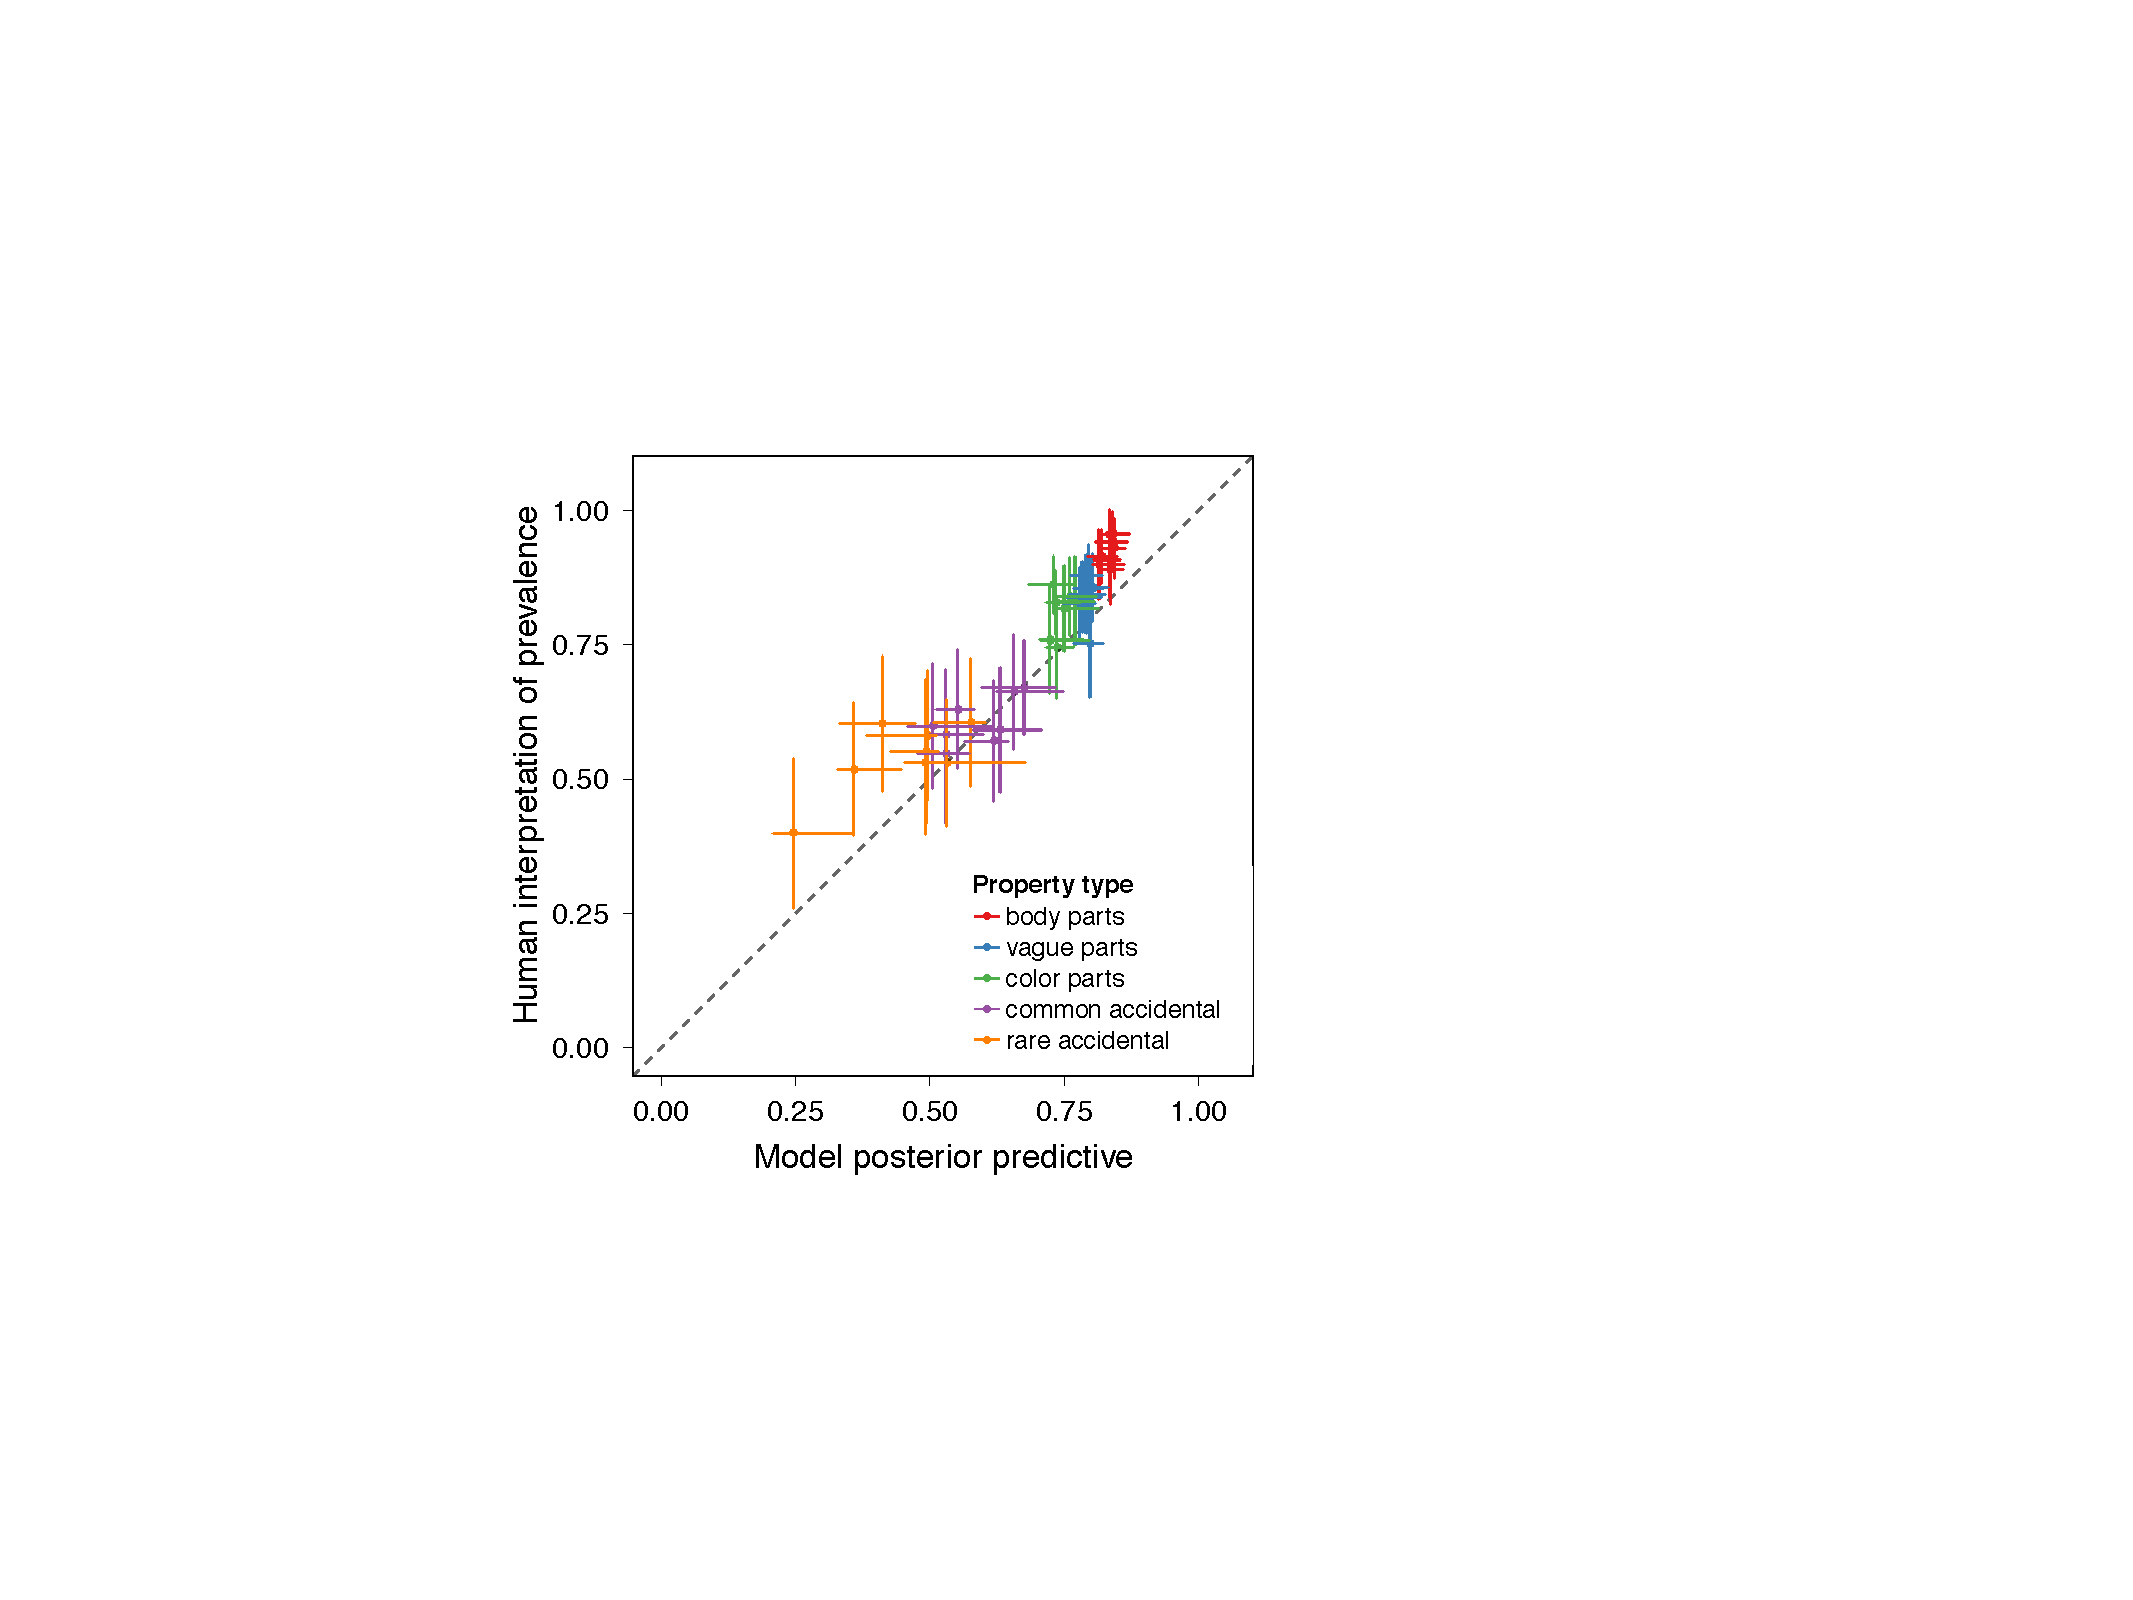
\includegraphics[width=0.5\columnwidth]{implied-byItem-mh100kX2b.pdf}
    \caption{Human interpretation of prevalence upon hearing a generic compared with the $L_1$ model posterior predictive. 
    Participants and the model interpret generics differently for different property types: Generics of biological properties (red, blue, green) have  strong interpretations while generics of accidental properties (purple, orange) are weak.}
    %    Error bars denote bootstrapped 95\% confidence intervals for the data and Bayesian 95\% credible intervals for the model.}
  \label{fig:impliedByItem}
\end{figure}

%Interestingly, we observe greater implied prevalence of common accidental properties than rare accidental properties, given our median split based on the prior elicitation task ($\beta=0.061; SE = 0.025; t(39) = 2.47; p = 0.018$) \footnote{These statistics are the result of a mixed-effects linear regression with a maximal mixed-effect structure: Random by-participant effects of intercept and slope}.
%Implications of generics of body parts was significantly greater than those of the biological properties used by \cite{Cimpian2010} (here, ``color parts'') ($\beta=0.118; SE = 0.024; t(39) = 4.74; p < 0.001$). 
%There was also a trending effect for the implications of vague body parts (e.g. curly fur) to be greater than those of color parts (e.g. yellow fur) ($\beta=0.032; SE = 0.016, t(54.8) = 1.95; p = 0.056$), possibly due to the belief that the same kind of animal can come in many different colors (e.g. dogs).
\begin{figure*}
\centering
    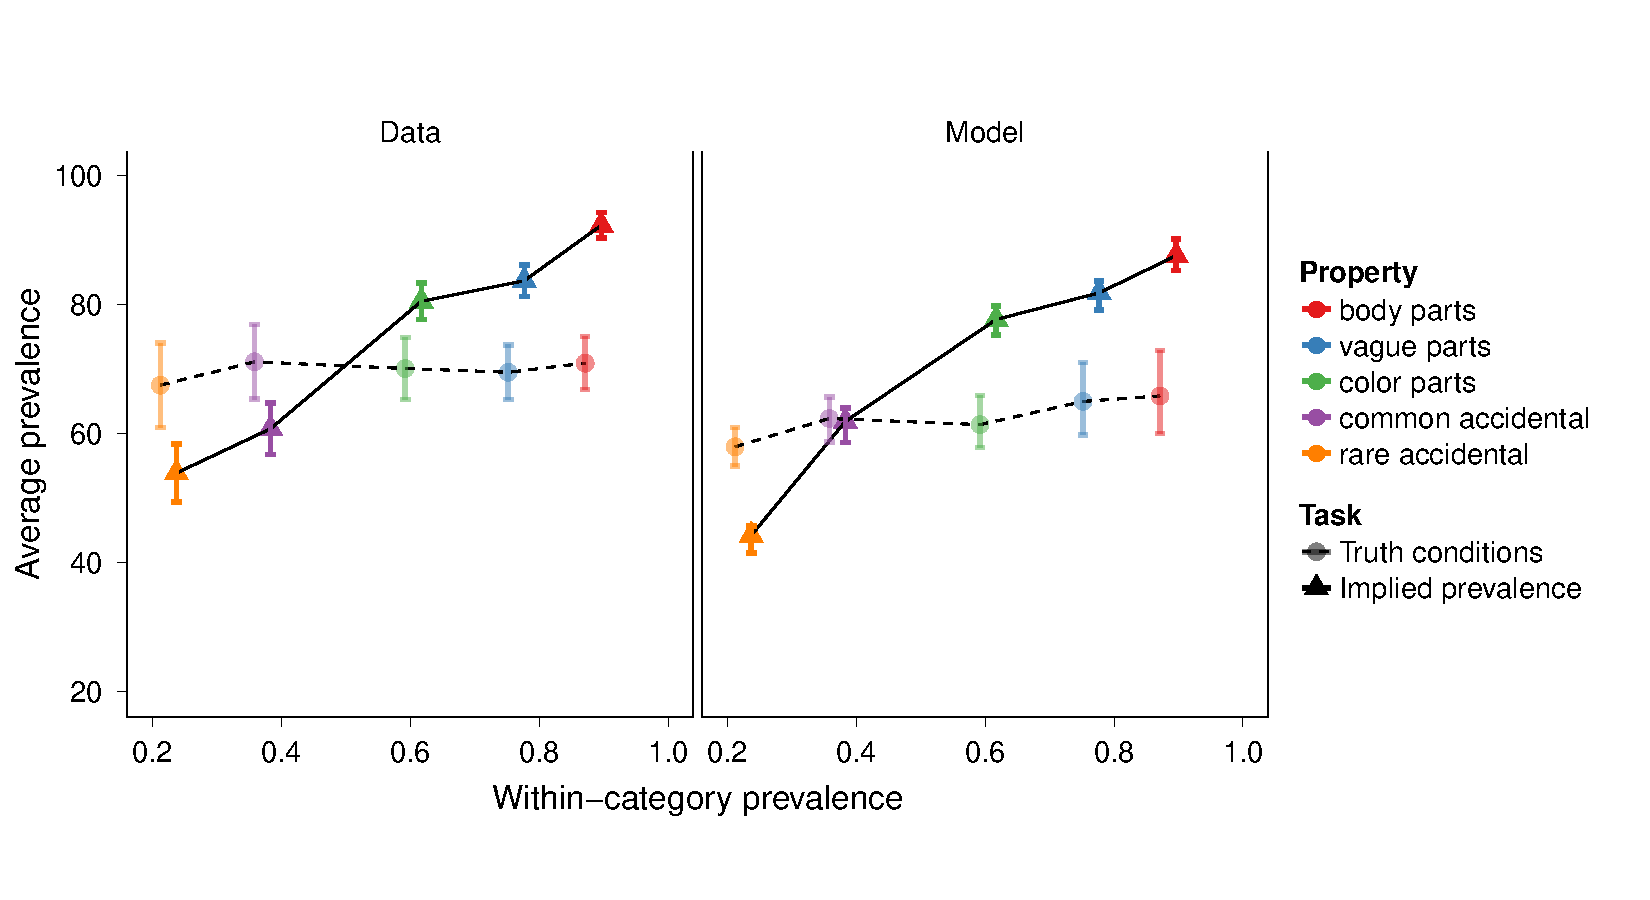
\includegraphics[width=\columnwidth]{asym-lines-data-model-2phi-2so-50kx3.pdf}
%    \includegraphics[width=1.2\columnwidth]{asym-lines-data-model.pdf}
    \caption{Human judgments and model predictions of prevalence implied by novel generic utterances (implied prevalence task; solid line) and average prevalence that leads to an acceptable generic utterance (truth conditions task; dotted line) as it relates to the \emph{a priori} mean prevalence when present $\gamma$.
    Expectations of prevalence are higher after hearing a generic than before hearing it (solid line compared to $y=x$ line; both for human data and model).
    %$y = x$ line denotes the prevalence inferred upon knowing the property is prettyesent in the kind. 
    %For each kind of property, the generic utterance implies a higher than expected prevalence.
    Generic statements about biological properties, imply that the property is widespread in the category, for both human participants and the model (solid line: red, blue and green). 
    Generics about accidental properties do not result in such a high implied prevalence (solid line: purple and orange).  
	While the implications of generic utterances are highly variable across the different types of properties, the average prevalence that leads to an acceptable generic does not vary, for participants or the model.
        %Generic statements are accepted for a range of prevalences, resulting in a intermediate average prevalence (dotted line) that deoesn't vary by property type for the truth conditions task. 
%    Error bars denote bootstrapped 95\% confidence intervals for the data and Bayesian 95\% credible intervals for the model.
%    \ndg{change x-axis label to "a priori expected prevalence" or something like that -- "within-category prevalence" is ambiguous.}
}
  \label{fig:exp2b}
\end{figure*}


%Consistent with the effects reported by \cite{Cimpian2010}, biological properties (body, vague, and color parts) have stronger interpretations than their truth conditions would suggest (Figure \ref{fig:exp2b}; solid vs. dotted lines; green, blue and red points), whereas accidental properties receive more modest interpretations (orange and purple points).



%How does the model capture these fine-grained inferences that listeners draw?
%Consider again the belief distributions about the properties inferred from Expt.~2a (Figure \ref{fig:prior2}). 
%All of the properties have substantial mass at 0 (Figure \ref{fig:prior2} Left). 
%This gives the speaker validity in saying the generic at low prevalence levels (though the speaker's confidence in doing so increases as prevalence increases).
%The listener has the complementary task: She brings \emph{a priori} uncertainty about the generic threshold to the table.
%Consider what would happen if she inferred the most conservative threshold (0) and responded with the \emph{maximum a posteriori} (MAP) of the distribution. 
%A threshold of 0 produces Figure \ref{fig:prior2} (right), because it only rules out the possibility that 0\% of the category has the property. 
%The resulting peaks (MAPs) of the distributions are near 1 for biological properties (parts, color parts, vague parts) and around 10\% for accidental properties (both rare and common). This alone would produce variable interpretations. 
%Our listener, however, does something wiser: She integrates over her uncertainty about the threshold (believing the speaker to be not just truthful but informative as well), and produces interpretations that both take reflect the whole distribution.
%This results in subtle differences between the implications of body parts (e.g. ``Lorches have wings.'') and  color parts (e.g.``Lorches have purple wings.''), and differences in interpretations of rare and common accidental properties. 
%

\section*{General discussion}

We evaluated a theory of generic language derived from general principles of pragmatic language understanding using a simple but uncertain basic meaning---a threshold on property prevalence.
Our formal model is a minimal extension of the RSA theory of language understanding, together with an underspecified threshold semantics.
The model was able to explain two philosophical puzzles of generics: their extremely flexible truth conditions and the contrastingly strong interpretation of novel generics, both of which were revealed to depend in systematic ways on prior knowledge about properties. In addition, the formal model predicted the quantitative details of participants' judgments with high accuracy.

%generics have a simple but uncertain basic meaning---a threshold on property prevalence---which is refined by social reasoning.
%a minimal extension of a general-purpose probabilistic model of language understanding wherein social-cognitive mechanisms act on uncertainty in the meaning of a generic utterance to produce a less uncertain meaning.
%Model predictions for interpretation of generic sentences depend on the listener's beliefs about the property in question and the communicative force of a speech-act. 
%The model predicted participants' judgements with high quantitative accuracy for both goodness judgements for natural generic sentences, and interpretation of novel generic sentences.
%Our model both the role of the speaker to produce felicitous generic utterances and the role of the listener to interpret those utterances in context, with high quantitative accuracy.
%general-purpose language understanding mechanisms are 



%%this paragraph isn't needed and is confusing....
%Interpretation of generic language is strongly governed by listeners' beliefs about the domain in question. 
%The generic, it would seem, doesn't convey any additional information beyond what the liste	ner already knew about the domain.
%This shouldn't surprise us. 
%In much the same way, ``John is tall'' does not actually tell a listener about what \emph{tall} means\footnote{However, ``John is a person'' does tell a listener about what \emph{tall} means in ``John is tall''.}. 
%Rather, the listener is expected to come to the conversation with some beliefs about heights, and knowing that John is a person, be able to infer likely meanings for \emph{tall}.
\subsection*{Implications for development}

\subsection*{Relation to previous empirical work on prevalence in generics}

The truth conditions of generic language have been of interest to linguists and philosophers. 


How generic language gets interpreted has been of interest to psychologists because of its ubiquity in natural conversation as well as its role in the growth of category knowledge. 
\citeA{Gelman2002} was the first to demonstrate that children and adults believe the prevalence implied by a novel generic utterance (e.g. \emph{Bears like to eat ants.}) is high, but distinct from quantifier statements like ``some'' or ``all''. 
The properties used in this experiment were plausible construed as biological or essential \cite{Gelman2003}.
In Expt.~2, we showed how the structure of prevalence priors about biological properties leads to this inference.  

This early work was conceptually replicated by \citeA{Cimpian2010} with novel categories (e.g. \textsc{lorches}) and extended to show that the strong interpretation of generics could be weakened by predicating the kind with accidental properties (e.g. \emph{Lorches have muddy feathers.}).
Indeed, causal beliefs about kinds have been argued to be the driving force behind these these variable interpretations\cite{Gelman2007, Cimpian2010c}.
Our work formalizes the relation between causal beliefs about kinds, prevalence, and generic language, and we have shown how this framework supports these prior claims.


\subsection*{Generic identification}

The puzzle of generic \emph{meaning} is often contrasted with the problem of generic \emph{identification}. 
Within this line of thinking, a sentence is hard to identify as conveying a generic meaning because generic meaning can be signaled using a number of morphosyntactic forms. 
For example, both \emph{Dogs are friendly} and \emph{A dog is friendly} are thought to both signal a generic interpretation.
Additionally, the morphosyntax alone is not a sufficient cue to generic meaning: \emph{Dogs are friendly} conveys a generic meaning while \emph{Dogs are on my front lawn} does not.

\citeA{Declerck1991} suggests that generic and nongeneric bare plurals can be treated in the same way, and that pragmatic considerations may resolve interpretative differences. 
We support this idea.
Consider, for example, the likely prevalence of animals on your front lawn. 
It is extremely unlikely for there to be many instances of \emph{any} animal on your front lawn (due to the spatial constraints of your lawn, and the lack of any good reason for an animal to be on your lawn). 
Thus, the prevalence prior would likely resemble that of an accidental property (Expt.~2a).
The $L_1$ listener model would in this case, interpret that bare plural as implying that just a few instances of dogs were on your front lawn. 


\subsection*{Implications for conceptual structure}


Previous psychological and philosophical work on generics has looked beyond prevalence and focused on conceptual distinctions and relations \cite{Gelman2003,Prasada2013,Leslie2007,Leslie2008}. 
\citeauthor{Prasada2013} has argued for a distinction between \emph{characteristic} properties (e.g.~\emph{Diapers are absorbent.}) and\emph{statistical} properties (e.g.~\emph{Diapers are white.}).
Leslie suggests information that is striking (e.g.~\emph{Tigers eat people.}) is useful and thus permitted to be a generic.
Gelman outlines how generics tend to express \emph{essential} qualities that are relatively timeless and enduring. 
We do not disagree with these claims. 
Rather than carve out the distinctions amongst generics, we highlight what is shared. 
%, and that generic language can increase the psychological coherence of a category.
%\citeA{GelmanEtAl2004} finds that child-parent conversations contain many more generics about animal kinds than about artifact kinds, possibly owing to the belief that animal kinds are more richly structured than artifact kinds. 
%Where in the prevalence-based semantics could such conceptual distinctions come into play?
Our approach makes the strong claim that beliefs about prevalence are the connective tissue between conceptual knowledge and generic language.
That is, the effect of conceptually meaningful differences on generic language is predicted to be mediated by differences in corresponding prevalence distributions.
And though prevalence may not be consciously considered when thinking about generics, the theory presented here suggests that this statistical information is along for the ride. 
Indeed, we found that empirical prevalence distributions are structured in a way that reflects intuitions about causal mechanisms underlying different properties.
It is plausible that richer conceptual knowledge also influences these distributions, such as higher-order conceptual knowledge about the nature of properties and categories \cite{Gelman2003,Keil1992}. 


\mht{Predictive probability is the mediatory between conceptual structure and generic language. Thus, differences in conceptual structure give rise to differences in predictive probability and generic language. It has been argued that conceptual structure can be represented by probabilisitic causal models \cite{Pearl, Gopnik, Goodman2015}. This is suggestive evidence for such a representation.}

\subsection*{Subjective probability and cue validity}

It is also important to note that our approach is based on \emph{subjective} probability, and not mere frequency.
This difference would be most apparent when abstract intuitive theories lead us to reject observed frequencies in forming our subjective probabilities. For instance, because we believe that social security numbers have no influence on selection for the Supreme Court, even if we find out that all Supreme Court justices have even social security numbers, we will assign about 50\% subjective probability to the next justice having an even number; we will thus reject the generic \emph{Supreme Court Justices have even social security numbers}. (If we learned much more surprising information, such as all justices having prime numbers, we might revise our theory, for instance appealing to a conspiracy, and then accept the generic.)
Further research will be needed to explore the predicted relationship between conceptual distinctions, subjective probabilities for prevalence, and generic language.



%Beliefs about prevalence in our approach are represented as probability distributions, a framework that is useful for representing rich, structured knowledge of the world \cite{Goodmanconcepts}. 




%
%For example, communicating subjective probability should be useful for future prediction and so if speakers hold the higher-order belief that some observations or states are transient and not predictive of future events (e.g. all U.S. Supreme Court Justices having at this moment social security numbers that are all prime numbers), their estimates of the subjective probability to communicate will be less influenced by this state; this will cause speakers to hesitate to assert the corresponding generic (\emph{Supreme Court Justices have prime numbered social security numbers}).


%To highlight one example, individuals may believe some observations are the result of accidents and are not predictive of future instances (e.g. all of the Supreme Court Justices having even-numbered social security numbers). 
%The corresponding generic (i.e. \emph{Supreme Court Justices have even-numbered social security numbers.}) may lack support because the corresponding conceptual models do not have any strong causal mechanism that could have given rise to the observation, and thus the prevalence of the property in the future (i.e. the predictive prevalence) will not be similar to the present prevalence. 
%In our experiments, we have focused on properties that are plausibly construed of as essential (e.g. \emph{lays eggs}, \emph{has feathers}) and thus predictive of future instances. 
%We found that a set of plausibly temporary properties (e.g. \emph{has muddy feathers}) are interpreted as implying a much lower percentage of the kind with the property than the biological properties, suggestive that the accidental nature of the property influences interpretations of prevalence.


%The results of these studies, as well  future research and model development.

%How interlocutors arrive at estimates of the prevalence, and what other inferences are licensed in a context, may be the result of a deeper conceptual model of the world. 

It might seem paradoxical that a part of language that is so common in communication and central to learning should be vague. 
Shouldn't speakers and teachers want to express their ideas as crisply as possible?
To the contrary, underspecification can be efficient, given that context can be used to resolve the uncertainty \cite{Piantadosi2012}.
In our work, context takes the form of a listener and speaker's shared beliefs about the property in question. 
By leveraging this common ground, generics provide a powerful way to communicate and learn generalizations about categories, 
which would be difficult or costly to learn through direct experience.
%This, coupled with standard inferences from conversational pragmatics, allows the listener to arrive at a specific meaning of the otherwise underspecified utterance.
The dark side of this flexibility is the potential for miscommunication or deceit: A speaker might assert a generic utterance that he himself would not accept, conveying a too-strong generalization to a na\"{i}ve listener.  
Our model predicts this potential particularly for properties which, when present, are widespread in a category---we showed that biological properties are believed to have this distribution, but many properties of social categories may as well \cite{Cimpian2011a,Cimpian2012b,Rhodes2012}.
%This listener would then have a belief distribution even further from the truth. 


Categories are inherently unobservable. 
You cannot see the category \textsc{dog}, only some number of instances of it.
Yet we easily talk about these unobservables, conveying hard-won generalizations to each other and down through generations.
The theory presented here gives one explanation of how we do so, providing a computational perspective on how category generalizations are conveyed and how beliefs play a central role in understanding language.






%\section*{Materials}
%%\begin{materials}
%%Details are given in the {\it SI Materials and Methods}.
%\subsection{Generics model}
%The generics model was implemented using the probabilisitic programming language WebPPL \cite{dippl}. 
%The model, once $P(x)$ is fixed, has one free parameter: the speaker rationality parameter $\lambda$ in Eq.~\ref{eq:S1}. 
%Because $\lambda$ is not of theoretical interest here, it is marginalized in accord with Bayesian data analysis principles \cite{LW2014}.
%Both the prevalence  x$\in$[0, 1]  and the threshold  $\theta \in$[0, 1] were discretized to permit exact enumeration of the posterior.
%The prevalence scale was discretized into 11 bins --- \{0, 0.01, 0.1, 0.2, ... , 0.8, 0.9, 0.99\} --- and the threshold scale into 10 bins ---  \{0, 0.1, 0.2, ... , 0.8, 0.9\}. 
%The results are the same when a 21, 20 bin discretization is used. 
%A fully specified version of the generics model, as well as the structured prior model (described below), can be found at http://forestdb.org/models/generics.html. 









%\appendix[Structured, Bayesian model of the prior elicitation task]


%\end{materials}
%
%\begin{acknowledgments}

\subsubsection*{Author contributions}
M. H. Tessler and N. D. Goodman developed theory and the study concept and design.
M. H. Tessler performed research and analyzed data.
M. H. Tessler and N. D. Goodman wrote the paper.

\subsubsection*{Acknowledgements}

This work was supported in part by National Science Foundation Graduate Research Fellowship DGE-114747 (to M.H.T.),
by John S. McDonnell Foundation Scholar Award 220020252 (to N.D.G.) and 
Office of Naval Research Grant N00014-13-1-0788 (to N.D.G.)

%\end{acknowledgments}
%

%\begin{thebibliography}{10}
%
%\bibitem{Carlson1977}
%Carlson GN (1977) Reference to kinds in english, Ph.D. thesis (University of Massachusetts, Amherst).
%
%\bibitem{Leslie2008}
%Leslie SJ (2008) {Generics: Cognition and acquisition}.
%\newblock {\em Philosophical Review} 117(1).
%
%\bibitem{Behrens2005}
%Behrens L (2005) {Genericity from a cross-linguistic perspective}.
%\newblock {\em Linguistics} 43(2):275--344.
%
%\bibitem{Carlson1995}
%Carlson GN, Pelletier FJ (1995) {\em The generic book.}
%\newblock (Chicago University Press).
%
%\bibitem{Gelman2004}
%Gelman SA (2004) {\em Learning words for kinds: Generic noun phrases in
%  acquisition}.
%\newblock (MIT Press), pp. 445--484.
%
%\bibitem{Gelman2008}
%Gelman SA, Goetz PJ, Sarnecka BW, Flukes J (2008) {Generic Language in
%  Parent-Child Conversations}.
%\newblock {\em Language Learning and Development} 4(1):1--31.
%
%\bibitem{Cimpian2008}
%Cimpian A, Markman EM (2008) {Preschool children's use of cues to generic
%  meaning}.
%\newblock {\em Cognition} 107:19--53.
%
%\bibitem{GelmanEtAl2004}
%Gelman SA, Taylor MG, Nguyen SP, Leaper C, Bigler RS (2004) {Mother-child
%  conversations about gender: Understanding the acquisition of essentialist
%  beliefs}.
%\newblock {\em Monographs of the Society for Research in Child Development}
%  69(1):vii, 116--127.
%
%\bibitem{Rhodes2012}
%Rhodes M, Leslie SJ, Tworek CM (2012) {Cultural transmission of social
%  essentialism}.
%\newblock {\em Proceedings of the National Academy of Sciences}
%  109(34):13526--13531.
%
%\bibitem{Leslie2015}
%Leslie SJ, Cimpian A, Meyer M, Freeland E (2015) {Expectations of brilliance
%  underlie gender distributions across academic disciplines}.
%\newblock {\em Science} 347(6219):262--265.
%
%\bibitem{Cimpian2010motivation}
%Cimpian A (2010) {The impact of generic language about ability on children's
%  achievement motivation.}
%\newblock {\em Developmental psychology} 46(5):1333--1340.
%
%\bibitem{Gelman2002}
%Gelman SA, Star JR, Flukes JE (2002) {Children's Use of Generics in Inductive
%  Inferences}.
%\newblock {\em Journal of Cognition and Development} 3(2):179--199.
%
%\bibitem{Cimpian2010}
%Cimpian A, Brandone AC, Gelman SA (2010) {Generic statements require little
%  evidence for acceptance but have powerful implications.}
%\newblock {\em Cognitive science} 34(8):1452--1482.
%
%\bibitem{Brandone2014}
%Brandone AC, Gelman SA, Hedglen J (2014) {Children's Developing Intuitions
%  About the Truth Conditions and Implications of Novel Generics Versus
%  Quantified Statements.}
%\newblock {\em Cognitive science} pp. 1--28.
%
%\bibitem{Carlson1995essay}
%Carlson GN (1995) Truth conditions of generic sentences: Two contrasting views
%  in {\em The Generic Book}, eds.{} Carlson GN, Pelletier FJ.
%\newblock (Univ. of Chicago Press), pp. 224--38.
%
%\bibitem{Prasada2000}
%Prasada S (2000) {Acquiring generic knowledge}.
%\newblock {\em TiCS} 4(2):66--72.
%
%\bibitem{Prasada2012}
%Prasada S, Hennefield L, Otap D (2012) {Conceptual and Linguistic
%  Representations of Kinds and Classes}.
%\newblock {\em Cognitive Science} 36(7):1224--1250.
%
%\bibitem{Clark1996}
%Clark HH (1996) {\em Using language}.
%\newblock (Cambridge University Press).
%
%\bibitem{Grice1975}
%Grice HP (1975) {\em Logic and conversation.}
%\newblock (Blackwell).
%
%\bibitem{Levinson2000}
%Levinson S (2000) {\em Presumptive meanings: The theory of generalized
%  conversational implicature}.
%\newblock (The MIT Press).
%
%\bibitem{Frank2012}
%Frank MC, Goodman ND (2012) Predicting pragmatic reasoning in language games.
%\newblock {\em Science} 336(6084).
%
%\bibitem{Goodman2013}
%Goodman ND, Stuhlm{\"u}ller A (2013) Knowledge and implicature: Modeling
%  language understanding as social cognition.
%\newblock {\em Topics in Cognitive Science}.
%
%\bibitem{Cohen1999}
%Cohen A (1999) {Generics, Frequency Adverbs, and Probability}.
%\newblock {\em Linguistics and Philosophy} 22.
%
%\bibitem{Lassiter2013}
%Lassiter D, Goodman ND (2013) {\em Context, scale structure, and statistics in
%  the interpretation of positive-form adjectives}.
%
%\bibitem{Lassiter2015}
%Lassiter D, Goodman ND (2015) Adjectival vagueness in a bayesian model of
%  interpretation.
%\newblock {\em Synthese}.
%
%\bibitem{Degen2014}
%Degen J, Goodman ND (2014) {\em Lost your marbles? The puzzle of dependent
%  measures in experimental pragmatics}.
%
%\bibitem{Griffiths2005}
%Griffiths TL, Tenenbaum JB (2005) {Structure and strength in causal induction.}
%\newblock {\em Cognitive psychology} 51(4):334--84.
%
%\bibitem{hurdleModels}
%Rose CE, Martin SW, Wannemuehler KA, Plikaytis BD (2006) On the use of
%  zero-inflated and hurdle models for modeling vaccine adverse event count
%  data.
%\newblock {\em Journal of biopharmaceutical statistics} 16(4):463--481.
%
%\bibitem{LW2014}
%Lee MD, Wagenmakers E (2014) {\em Bayesian Cognitive Modeling: A Practical
%  Course}.
%\newblock (Cambridge University Press, Cambridge).
%
%\bibitem{Prasada2013}
%Prasada S, Khemlani S, Leslie SJ, Glucksberg S (2013) {Conceptual distinctions
%  amongst generics.}
%\newblock {\em Cognition} 126(3):405--22.
%
%\bibitem{Nisbett1983}
%Nisbett RE, Krantz DH, Jepson C, Kunda Z (1983) {The use of statistical
%  heuristics in everyday inductive reasoning.}
%\newblock {\em Psychological Review} 90(4):339--363.
%
%\bibitem{Gelman2003}
%Gelman SA (2005) {\em Essential Child: Origins of Essentialism in Everyday
%  Thought.}
%\newblock (Oxford University Press).
%
%\bibitem{Leslie2007}
%Leslie SJ (2007) {Generics and the Structure of the Mind}.
%\newblock {\em Philosophical Perspectives} 21(1):375--403.
%
%\bibitem{Goodmanconcepts}
%Goodman ND, Tenenbaum JB, Gerstenberg T (2015) {\em Concepts in a probabilistic
%  language of thought}.
%\newblock (MIT Press).
%
%\bibitem{Keil1992}
%Keil FC (1992) {\em Concepts, kind, and cognitive development.}
%\newblock (MIT Press).
%
%\bibitem{Piantadosi2012}
%Piantadosi ST, Tily H, Gibson E (2012) {The communicative function of ambiguity
%  in language}.
%\newblock {\em Cognition} 122(3):280--291.
%
%\bibitem{Cimpian2011a}
%Cimpian A, Markman EM (2011) {The Generic/Nongeneric Distinction Influences How
%  Children Interpret New Information About Social Others}.
%\newblock {\em Child Development} 82(2):471--492.
%
%\bibitem{Cimpian2012b}
%Cimpian A, Mu Y, Erickson LC (2012) {Who Is Good at This Game? Linking an
%  Activity to a Social Category Undermines Children's Achievement}.
%\newblock {\em Psychological Science} 23(5):533--541.
%
%\bibitem{dippl}
%Goodman ND, Stuhlm\"{u}ller A (2014) {The Design and Implementation of
%  Probabilistic Programming Languages} (\url{http://dippl.org}).
%\newblock Accessed: 2015-7-17.
%
%\end{thebibliography}

%\end{article}

%\begin{figure*}
%\centering
%    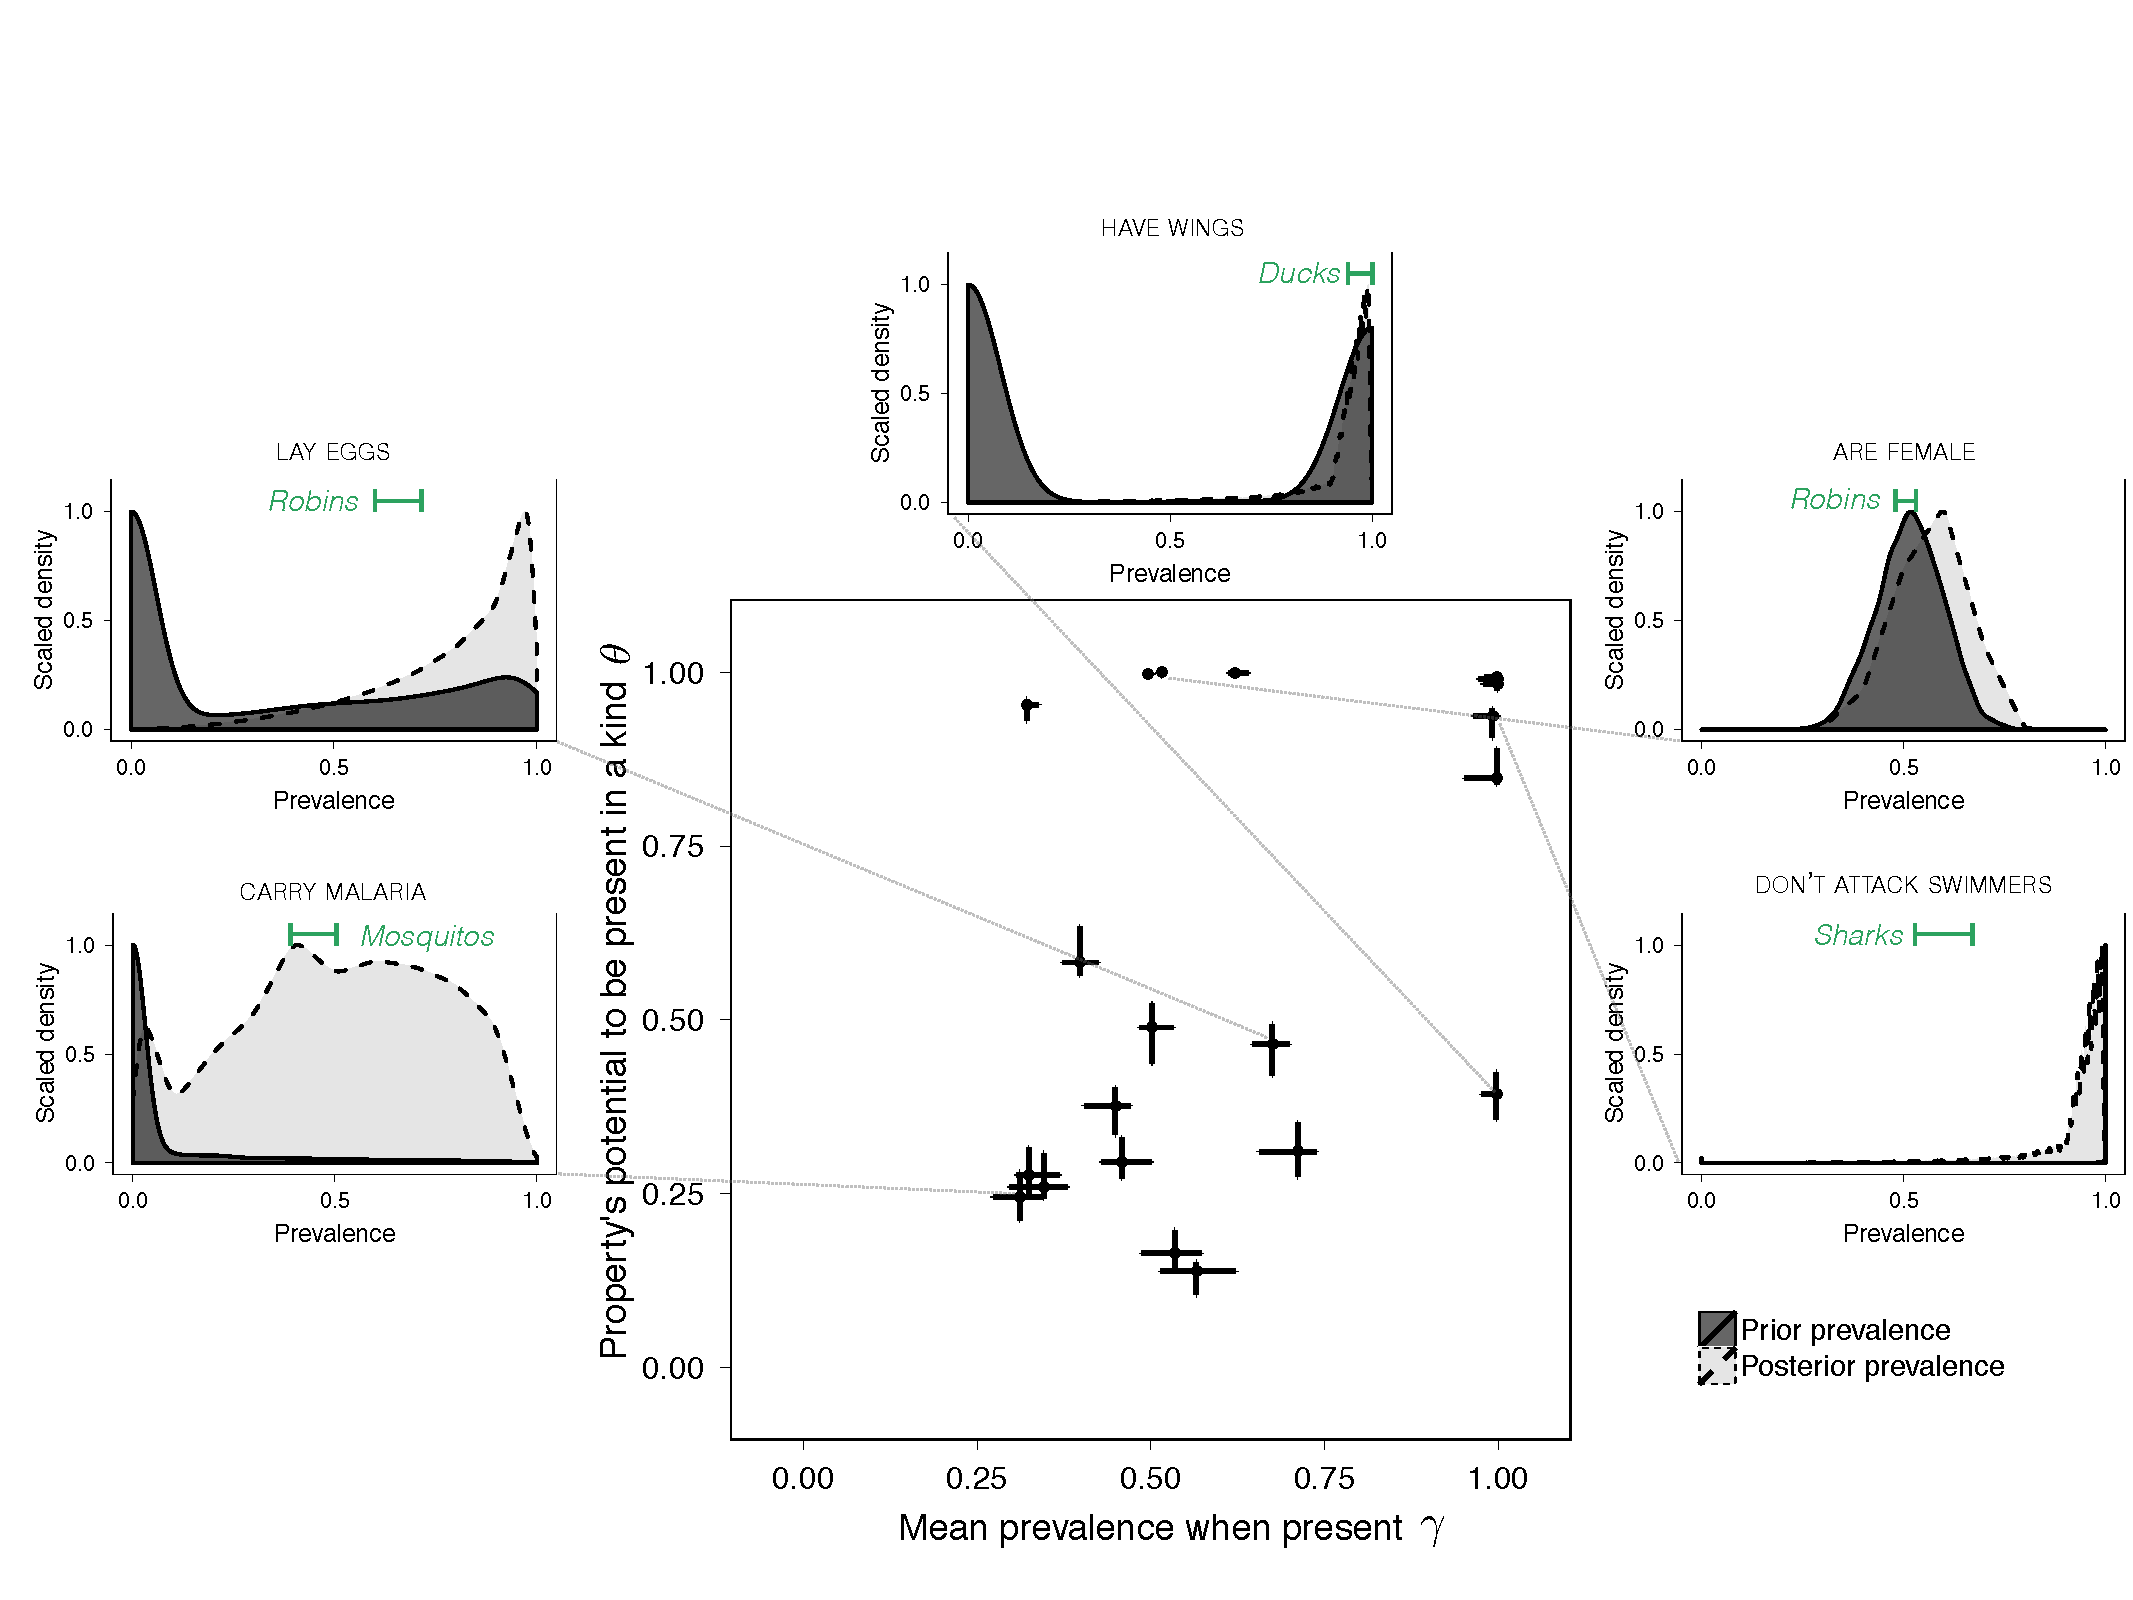
\includegraphics[width=\columnwidth]{prevalence-scatter-wDists2.pdf}
%    \caption{Prevalence prior distributions empirically elicited for twenty-one animal properties.
%    Prior distributions are summarized by $\theta$----a property's potential to be present in a category----and $\gamma$----the mean prevalence when it is possible for the property to be present in a category.
%    Inset plots display example empirical prior distributions over prevalence together with corresponding $L_1$ model predictions: the posterior after hearing a generic utterance. 
%    Intervals on the top of plots show human beliefs about the prevalence of the property within a target category.
%%    Posterior distributions show what happens to a listener's belief about the prevalence after hearing the associated generic. 
%    Felicitous generic utterances result when the target prevalence is more likely under the posterior than under the prior.
% %   \ndg{should mark the observed within-category prevalence for target kinds in pop-outs? or maybe one of the axes of main plot should be that?}
%     Error bars denote 95\% Bayesian credible intervals.
%    }
%  \label{fig:priors1a}
%\end{figure*}
%
%\begin{figure}
%\centering
%    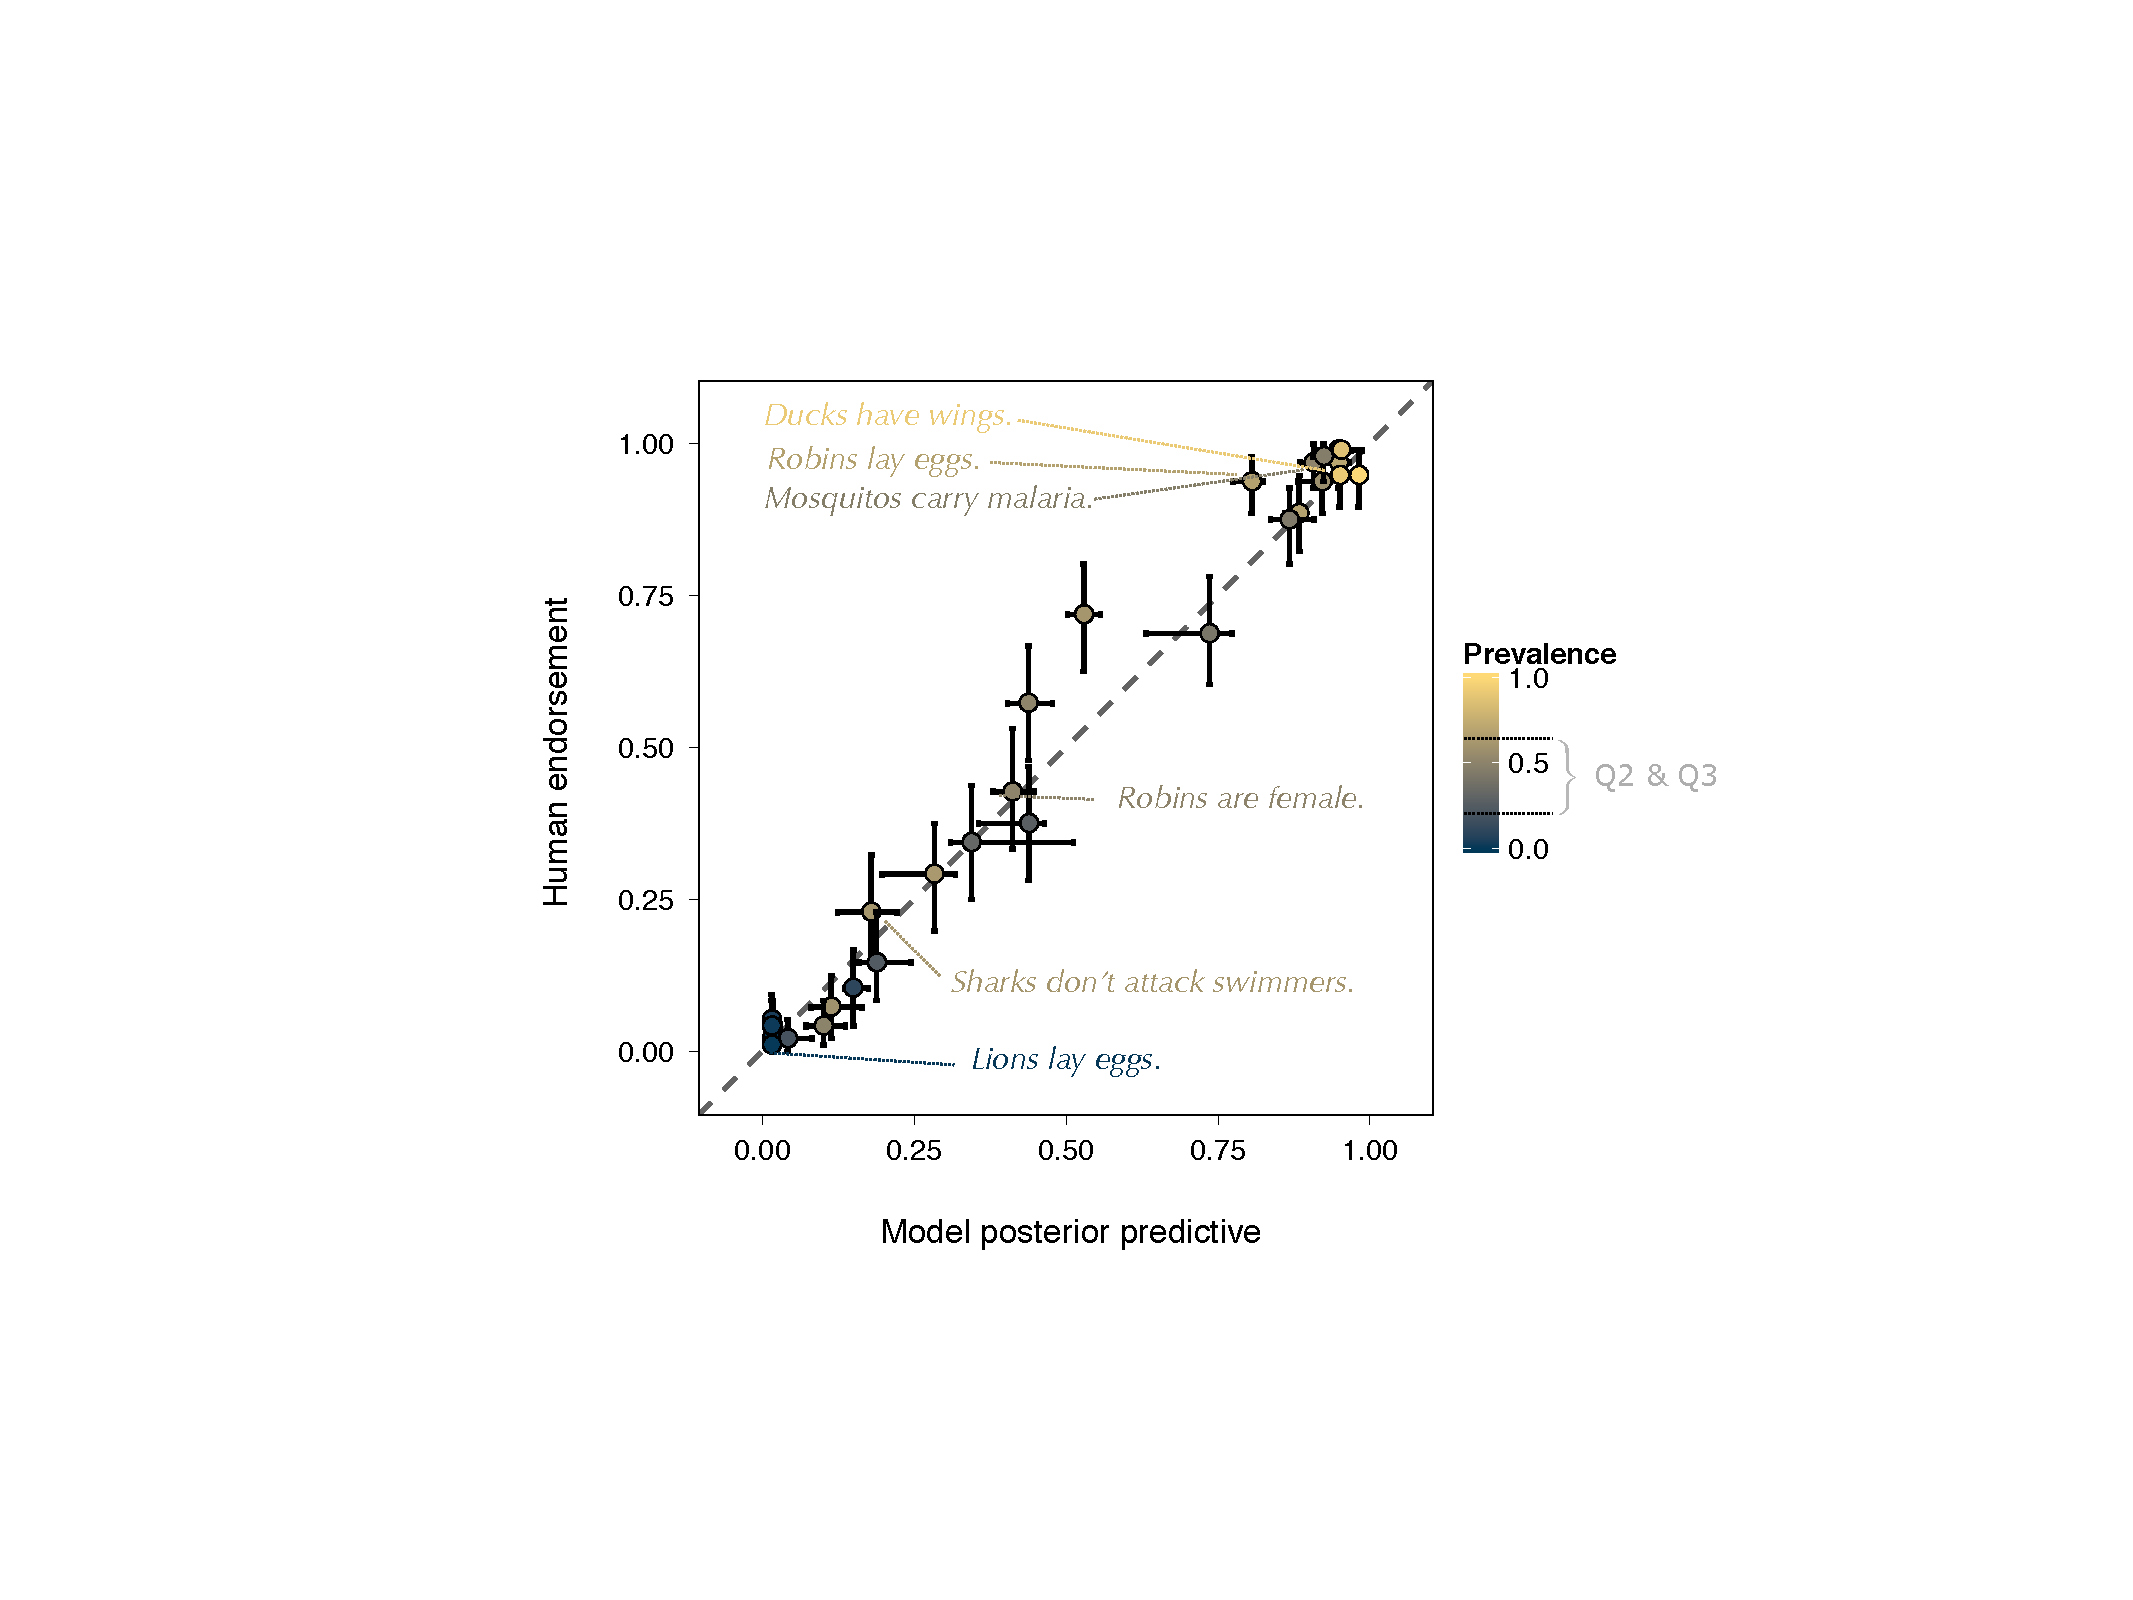
\includegraphics[width=0.49\columnwidth]{truthjudge-scatter-wLabels.pdf}
%    \caption{Human acceptability judgments and model predictions for thirty generic utterances about familiar animals and properties. 
%    Color denotes target-category prevalence of the property, with darker colors indicating lower prevalence. 
%    Intermediate prevalences (quartiles 2 \& 3) are in intermediate shades (marked on color bar).
%    Error bars correspond with 95\% bootstrapped confidence intervals for the participant data and 95\% highest probability intervals for the model predictions.
%    }
%  \label{fig:modeldataBars}
%\end{figure}
%
%
%\begin{figure*}
%\centering
%    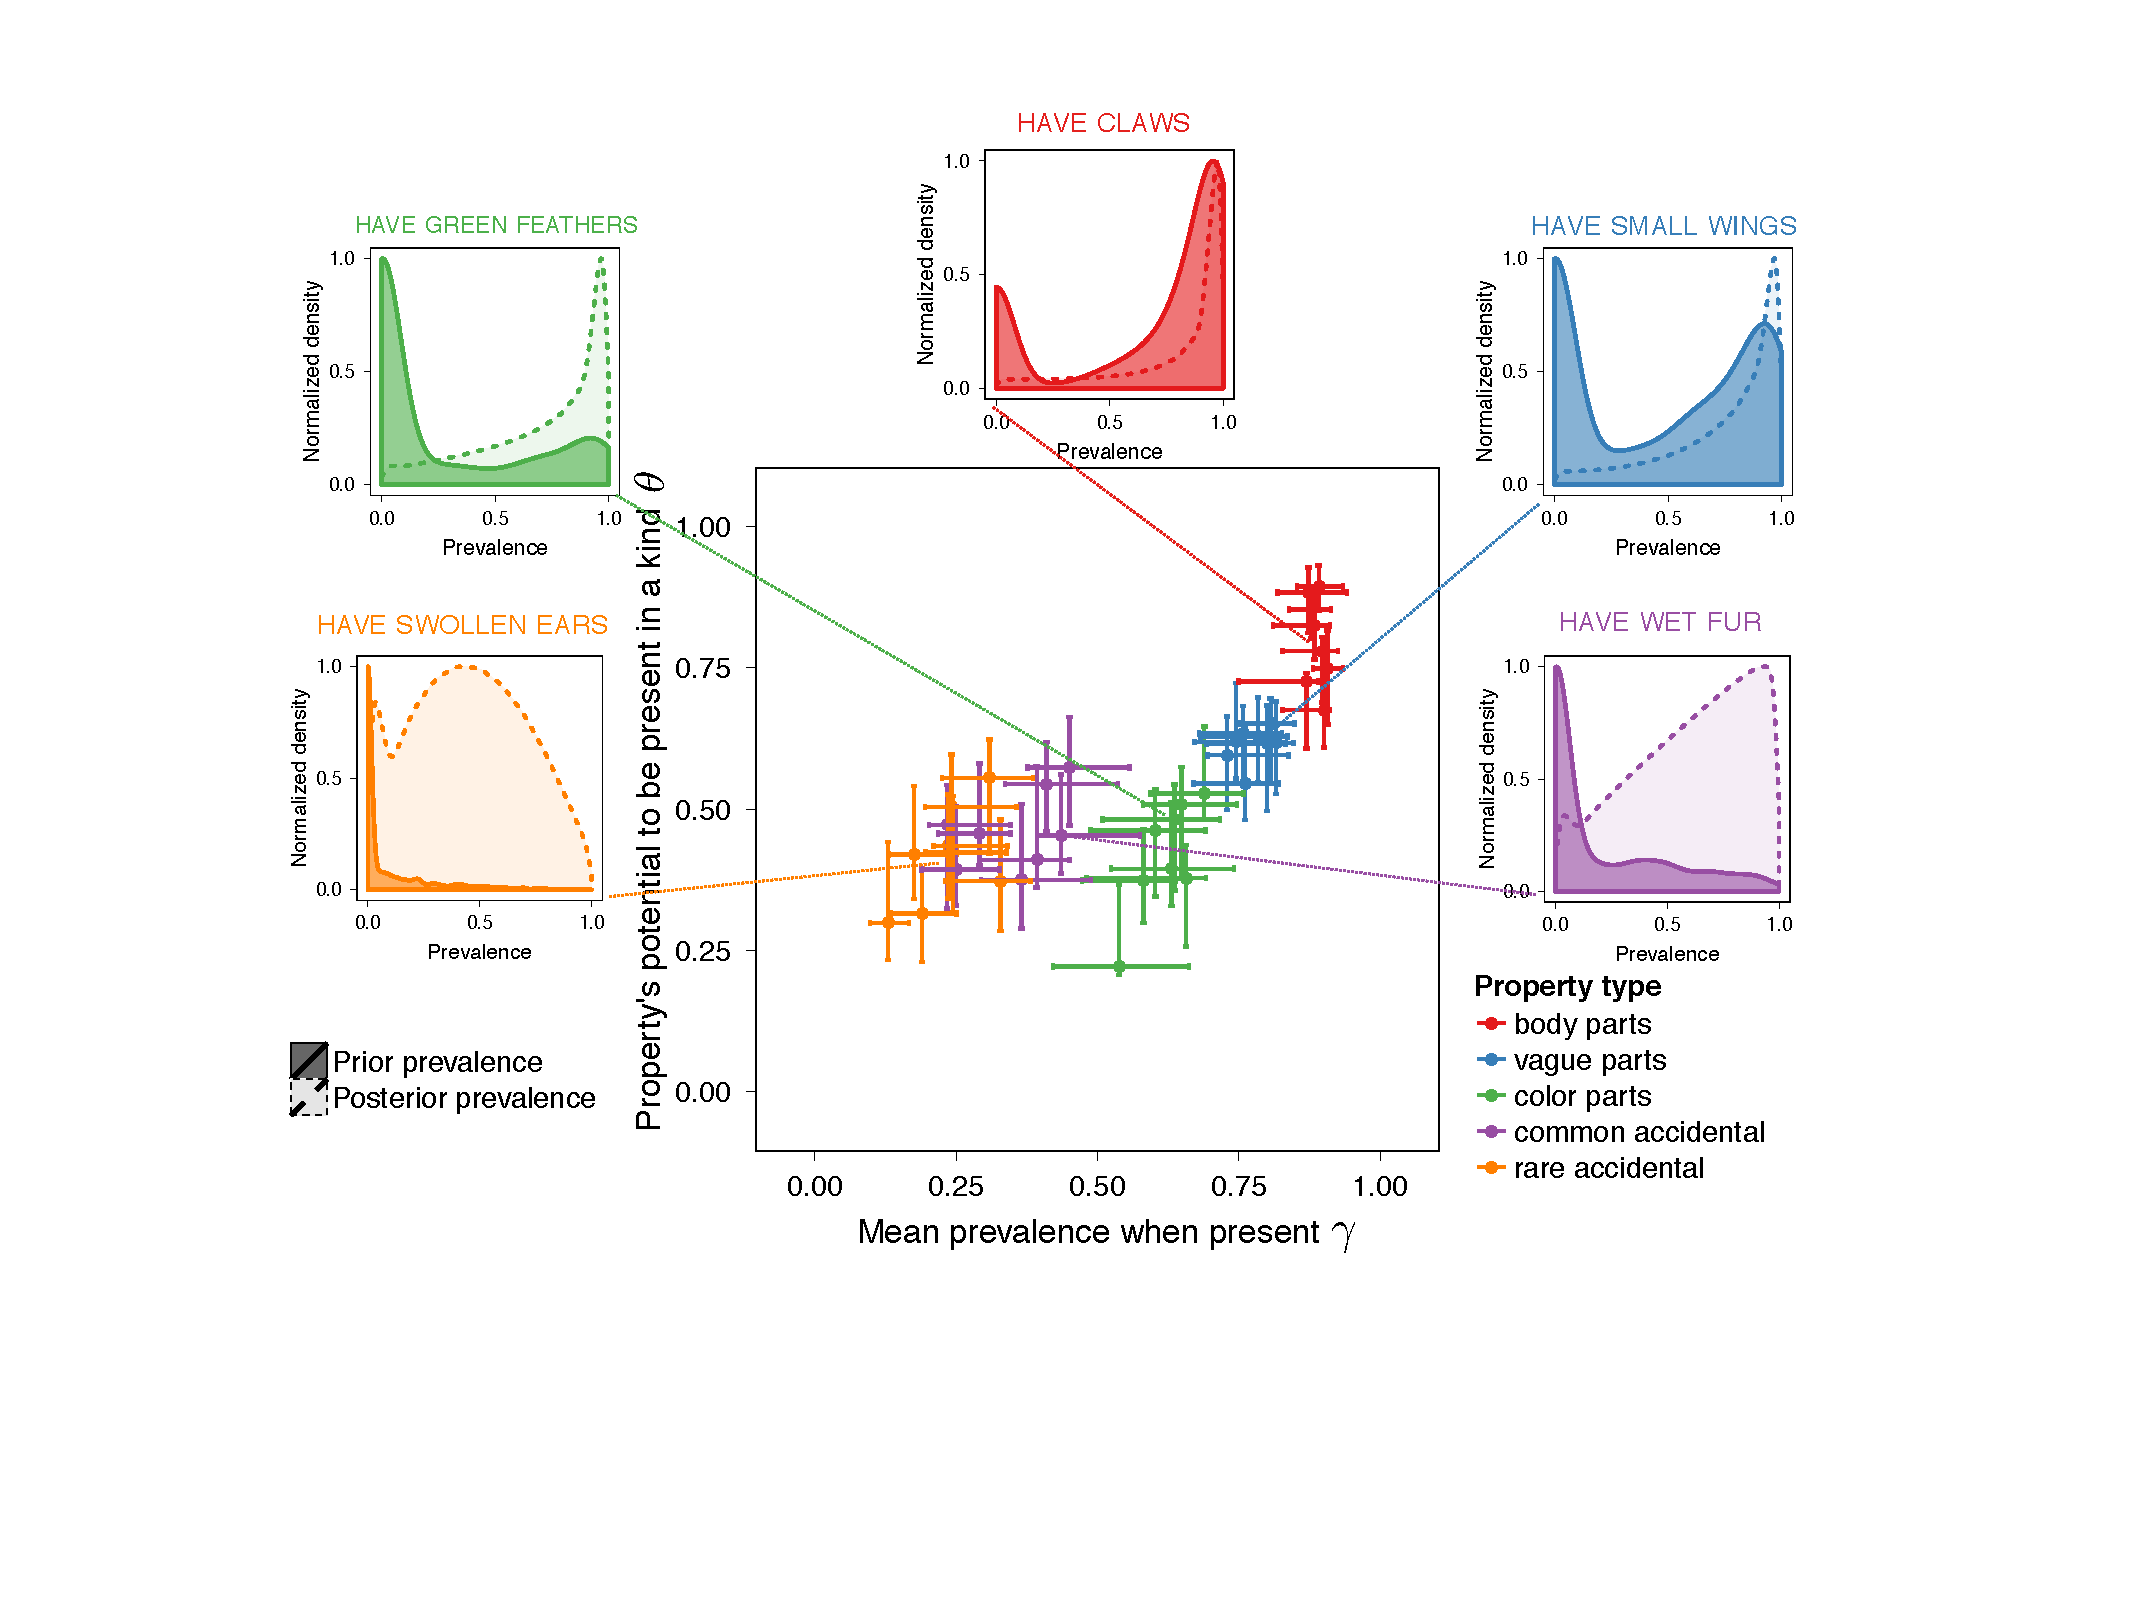
\includegraphics[width=\columnwidth]{prevalence-asymmetry-scatterwDists-byItem.pdf}
%    \caption{Prevalence prior distributions empirically elicited for 40 animal properties.
%    Parameters of the structured statistical model---$\theta$ and $\gamma$---reveal quantitative differences in beliefs about the prevalence of conceptually different types of properties (scatterplot). 
%    Inset plots show differences in shapes between biological properties (red, green, blue; bimodal) and accidental properties (orange, purple; unimodal).   
%  These differences give rise to the variability of interpretations of generic utterances. 
%      Error bars denote Bayesian 95\% credible intervals.
%  }
%  \label{fig:prior2}
%\end{figure*}
%
%
%\begin{figure}
%\centering
%    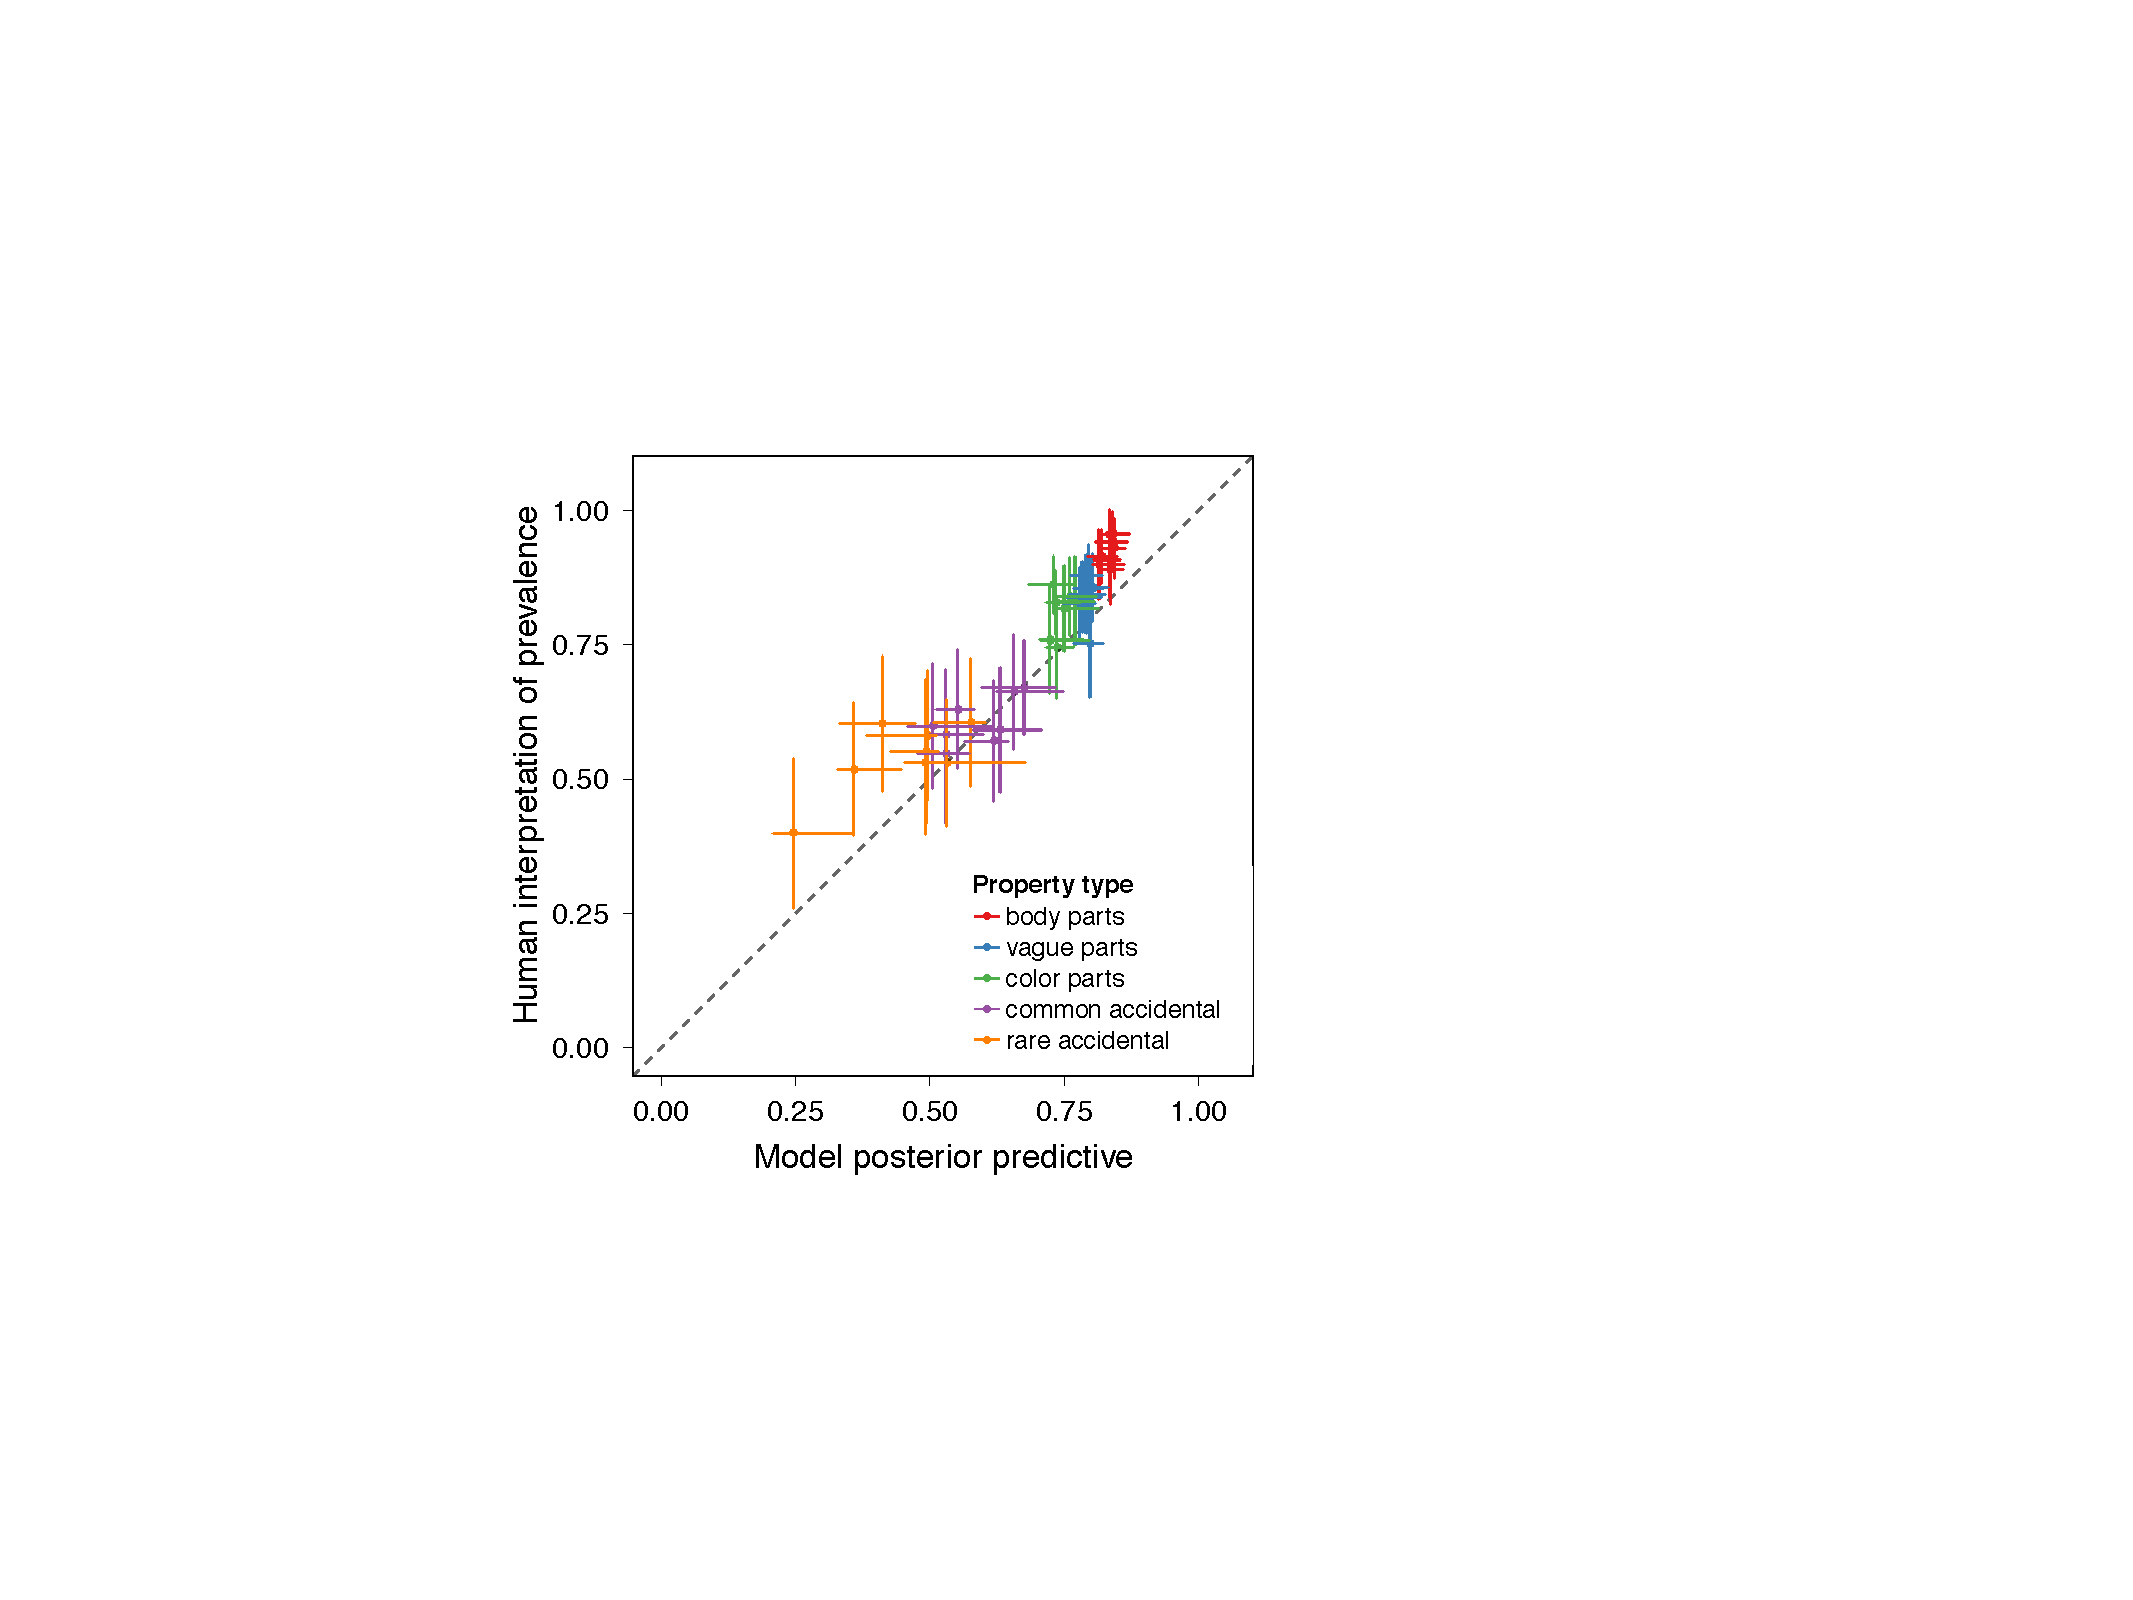
\includegraphics[width=0.48\columnwidth]{implied-byItem-mh100kX2b.pdf}
%    \caption{Human interpretation of prevalence upon hearing a generic compared with the $L_1$ model posterior predictive. 
%    Participants display graded endorsements of generics in terms of prevalence based on type of property (which is also associated with \emph{mean prevalence when present} $\gamma$, see Figure 3).
%    The model displays the same variability of interpretation, producing strong interpretations for generics of biological properties (red, blue, green) and weaker interpretations of generics of accidental properties (purple, orange).
%        Error bars denote bootstrapped 95\% confidence intervals for the data and Bayesian 95\% credible intervals for the model.}
%  \label{fig:impliedByItem}
%\end{figure}
%
%\begin{figure*}
%\centering
%    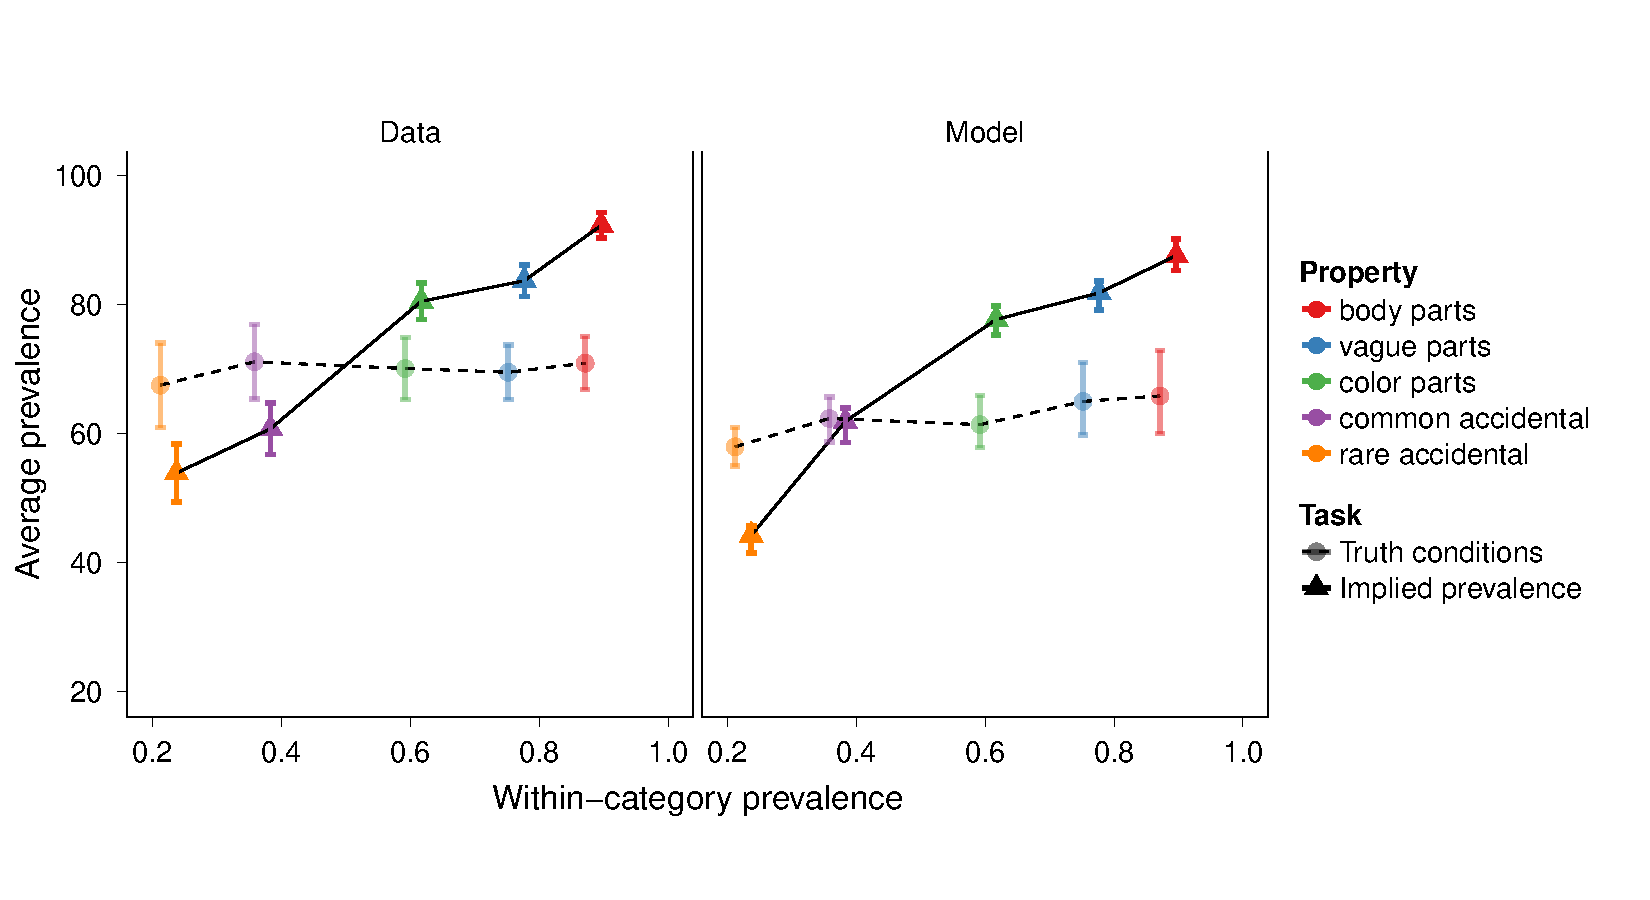
\includegraphics[width=\columnwidth]{asym-lines-data-model-2phi-2so-50kx3.pdf}
%    \caption{Human judgments and model predictions of prevalence implied by novel generic utterances (implied prevalence task; solid line) and average prevalence that leads to an acceptable generic utterance (truth conditions task; dotted line) as it relates to the \emph{a priori} mean prevalence when present $\gamma$.
%    Expectations of prevalence are higher after hearing a generic than before hearing it (solid line compared to $y=x$ line; both for human data and model).
%    %$y = x$ line denotes the prevalence inferred upon knowing the property is prettyesent in the kind. 
%    %For each kind of property, the generic utterance implies a higher than expected prevalence.
%    Generic statements about biological properties, imply that a high proportion of the category has the property, for both human participants and the model (solid line: red, blue and green). 
%    Generics about accidental properties do not result in such a high implied prevalence (solid line: purple and orange).  
%	While the implications of generic utterances are highly variable across the different types of properties, the average prevalence that leads to an acceptable generic does not vary, for participants or the model.
%        %Generic statements are accepted for a range of prevalences, resulting in a intermediate average prevalence (dotted line) that deoesn't vary by property type for the truth conditions task. 
%    Error bars denote bootstrapped 95\% confidence intervals for the data and Bayesian 95\% credible intervals for the model.
%%    \ndg{change x-axis label to "a priori expected prevalence" or something like that -- "within-category prevalence" is ambiguous.}
%}
%  \label{fig:exp2b}
%\end{figure*}
\newpage
\bibliographystyle{apacite}

\setlength{\bibleftmargin}{.125in}
\setlength{\bibindent}{-\bibleftmargin}

\bibliography{generics}

\end{document}


